% Remove the oneside option below for double sided printing (e.g. for final (post-viva) submission)
\documentclass[a4paper,12pt,oneside,openright]{book}
\usepackage[colorlinks=true, linkcolor=black!50!blue, urlcolor=blue, citecolor=blue, anchorcolor=blue]{hyperref}
\usepackage[font=small,labelfont=bf,margin=0mm,labelsep=period,tableposition=top]{caption}
% Preamble commands go here
\usepackage{graphicx,placeins}
\usepackage{afterpage}
\usepackage{epsfig,cite}
\usepackage{amssymb}
\usepackage{amsmath}
\usepackage{dsfont}
\usepackage{multirow}
\usepackage{url}
\usepackage[table]{xcolor}
\usepackage{breqn}
\usepackage{float}
\usepackage{afterpage}
\usepackage{gensymb}
\usepackage{url}
\usepackage{booktabs}
\usepackage{tikz}
\usetikzlibrary{arrows}
\usepackage{tikz-3dplot}
\usepackage{enumitem}
\usepackage{customisations}
\usepackage{mathtools}
\usepackage{slashed}
%\usepackage{subcaption}
\usepackage{subfig}
\usepackage{wrapfig}
\usepackage{textcomp} % textcomp provides extra text symbols (like a degrees celsius symbol)
% New commands
\def\truev{\mathcal{T}}
% COMMANDS
\def\smallfrac#1#2{\hbox{$\frac{#1}{#2}$}}
\def\half{\smallfrac{1}{2}}
\def\third{\smallfrac{1}{3}}
\def\quarter{\smallfrac{1}{4}}
\newcommand{\be}{\begin{equation}}
\newcommand{\ee}{\end{equation}}
\newcommand{\bs}{\begin{split}}
\newcommand{\es}{\end{split}}
\newcommand{\bdm}{\begin{dmath}}
\newcommand{\edm}{\end{dmath}}
\newcommand{\bea}{\begin{eqnarray}}
\newcommand{\eea}{\end{eqnarray}}
\newcommand{\bi}{\begin{itemize}}
\newcommand{\ei}{\end{itemize}}
\newcommand{\ben}{\begin{enumerate}}
\newcommand{\een}{\end{enumerate}}
\newcommand{\la}{\left\langle}
\newcommand{\ra}{\right\rangle}
\newcommand{\lc}{\left[}
\newcommand{\rc}{\right]}
\newcommand{\lp}{\left(}
\newcommand{\rp}{\right)}
\newcommand{\as}{\alpha_s}
\newcommand{\aq}{\alpha_s\left( Q^2 \right)}
\newcommand{\amz}{\alpha_s\left( M_Z^2 \right)}
\newcommand{\aqq}{\alpha_s \left( Q^2_0 \right)}
\newcommand{\aqz}{\alpha_s \left( Q^2_0 \right)}
\def\toinf#1{\mathrel{\mathop{\sim}\limits_{\scriptscriptstyle
{#1\rightarrow\infty }}}}
\def\tozero#1{\mathrel{\mathop{\sim}\limits_{\scriptscriptstyle
{#1\rightarrow0 }}}}
\def\toone#1{\mathrel{\mathop{\sim}\limits_{\scriptscriptstyle
{#1\rightarrow1 }}}}
\def\frac#1#2{{{#1}\over {#2}}}
\def\gsim{\mathrel{\rlap{\lower4pt\hbox{\hskip1pt$\sim$}}
    \raise1pt\hbox{$>$}}}         %greater than or approx. symbol
\def\lsim{\mathrel{\rlap{\lower4pt\hbox{\hskip1pt$\sim$}}
    \raise1pt\hbox{$<$}}}         %less than or approx. symbol
\newcommand{\mrexp}{\mathrm{exp}}
\newcommand{\dat}{\mathrm{dat}}
\newcommand{\one}{\mathrm{(1)}}
\newcommand{\two}{\mathrm{(2)}}
\newcommand{\art}{\mathrm{art}}
\newcommand{\rep}{\mathrm{rep}}
\newcommand{\net}{\mathrm{net}}
\newcommand{\stopp}{\mathrm{stop}}
\newcommand{\sys}{\mathrm{sys}}
\newcommand{\stat}{\mathrm{stat}}
\newcommand{\diag}{\mathrm{diag}}
\newcommand{\pdf}{\mathrm{pdf}}
\newcommand{\tot}{\mathrm{tot}}
\newcommand{\minn}{\mathrm{min}}
\newcommand{\mut}{\mathrm{mut}}
\newcommand{\partt}{\mathrm{part}}
\newcommand{\dof}{\mathrm{dof}}
\newcommand{\NS}{\mathrm{NS}}
\newcommand{\cov}{\mathrm{cov}}
\newcommand{\gen}{\mathrm{gen}}
\newcommand{\cut}{\mathrm{cut}}
\newcommand{\parr}{\mathrm{par}}
\newcommand{\val}{\mathrm{val}}
\newcommand{\tr}{\mathrm{tr}}
\newcommand{\checkk}{\mathrm{check}}
\newcommand{\reff}{\mathrm{ref}}
\newcommand{\Mll}{M_{ll}}
\newcommand{\extra}{\mathrm{extra}}
\newcommand{\draft}[1]{}
\newcommand{\comment}[1]{{\bf \it  #1}}
\def\beq{\begin{equation}}
\def\eeq{\end{equation}}

% Added by MU 
\def \a{\alpha}
\def \b{\beta}
\def \g{\gamma}
\def \z{\zeta}
\def \D{\Delta}
\def \t{{\bf T}} % vector of theoretical predictions
\def \c{{\bf c}} % vector of coefficients of theoretical predictions
\def \y{{\bf y}} % vector of experimental data
\def \s{{\bf \sigma}} % experimental covariance matrix
% Added by JR
\def\lapprox{\lower .7ex\hbox{$\;\stackrel{\textstyle <}{\sim}\;$}}
\def\gapprox{\lower .7ex\hbox{$\;\stackrel{\textstyle >}{\sim}\;$}}
\def\half{\smallfrac{1}{2}}
\def\GeV{{\rm GeV}}
\def\TeV{{\rm TeV}}
\def\ap{{a'}}
\def\vp{{v'}}
\def\e{\epsilon}
\def\d{{\rm d}}
\def\calN{{\cal N}}
\def\shat{\hat{s}}
\def\barq{\bar{q}}
\def\qq{q \bar q}
\def\uu{u \bar u}
\def\dd{d \bar d}
\def\pp{p \bar p}
\def\xa{x_{1}}
\def\xb{x_{2}}
\def\xaa{x_{1}^{0}}
\def\xbb{x_{2}^{0}}
\def\smx{\stackrel{x\to 0}{\longrightarrow}}
\def\Li{{\rm Li}}

\newcommand{\pmz}{{\pm}\hspace{-.9em}{\bigcirc}} 
%Alternatively: {\pm \atop 0}


\numberwithin{equation}{section}
\numberwithin{figure}{section}
\numberwithin{table}{section}

\newcommand{\tmop}[1]{\ensuremath{\operatorname{#1}}}
\newcommand{\tmtextit}[1]{{\itshape{#1}}}
\newcommand{\tmtextrm}[1]{{\rmfamily{#1}}}
\newcommand{\tmtexttt}[1]{{\ttfamily{#1}}}

\usepackage{tabularx}
\newcolumntype{C}[1]{>{\centering\arraybackslash}p{#1}}

% End preamble

% REPLACE THESE with your thesis title, your name and the date of submission of the thesis
\title{Theoretical Uncertainties in Parton Distribution Functions}
\author{Rosalyn Laura Pearson}
\date{May 2020} % of submission

\begin{document}

% Thesis front matter - title page, abstract, acknowledgements, declaration and table of contents
% See customisations.sty to modify the title page or declaration
\singlespacing
\maketitlepage
\frontmatter
\eighteenptleading
\chapter{Abstract}
We are now in the era of high precision particle physics, spurred on by a wealth of new data from the Large Hadron Collider (LHC). In order to match the precision set by modern experiments and test the limits of the Standard Model, we must increase the sophistication of our theoretical predictions. Much of the data available involve the interaction of protons, which are composite particles. These interactions are described by combining perturbative Quantum Chromodynamics (QCD) with parton distribution functions (PDFs), which encapsulate the non-perturbative behaviour. Increasing accuracy and precision of these PDFs is therefore of great value to modern particle physics.

PDFs are determined by multi-dimensional fits of experimental data to theoretical predictions from QCD. Uncertainties in PDFs arise from those in the experimental data and theoretical predictions, as well as from the fitting procedure itself. Those in the theory come from many sources. Here we consider two of the most important: the first are missing higher order uncertainties (MHOUs), arising due to truncating the predictions' perturbative expansion; the second are nuclear uncertainties, due to difficulty making predictions in a nuclear environment.

In this thesis we consider how to include theory uncertainties in PDF fits by constructing a theory covariance matrix and adding this to the experimental one. MHOUs are estimated and included as a proof of concept in next-to-leading order PDFs. We find that these capture many of the important features of the known PDFs at the next order above. We then investigate nuclear uncertainties, estimate their magnitude and assess their impact on the PDFs. Finally, we consider how to make predictions with theory uncertainties using PDFs which themselves include theory uncertainties. Here there are correlations between the PDFs and the predictions, which can lead to a shift in the predictions and their uncertainties, which can significantly improve their accuracy and precision.


\singlespacing
% Uncomment this line if you need to declare published work which forms part of the thesis
\declarationpublications{\cite{ }}
\makedeclaration

\chapter{Acknowledgements}

\noindent

\normalsize

First and foremost I would like to thank my supervisor, Richard Ball, for his support and guidance in this project, and for steering me towards a fascinating and cohesive area of research. I have benefited very much from his insightful perspective, and meticulous understanding of the interplay of ingredients in PDF fits. Important thanks also go to Emanuele Nocera, who helped me find my feet in the early days of my PhD, and has been immensely helpful and supportive throughout, above and beyond what I could have hoped for. Without him I am not sure I would be writing this thesis! Also to Zahari Kassabov for his perpetual presence on GitHub, answering thousands of questions and helping me to develop good coding practices. 

I have also met some lovely people in NNPDF, of which there are too many to list here. But in particular I would like to mention Mikey and Tommaso, the Edinburgh students in my year. They have helped me out more times than I can count with my research and with the code development, and I was very happy to share an office with them. I also really enjoyed collaborating closely with Cameron during the first couple of years. Thanks also go to Rabah and Shayan. Finally, I would like to thank Emma for helping me stick through the tougher moments, and providing mentorship from the year above. 

Outwith my PhD I have had a tough few years and I would like to thank my sister Julia, my partner Fred and my best friend Eleanor, all of whom I have also lived with. In particular, thanks to Eleanor for her help with the artwork for some of the figures. 

Finally, this research has been made possible through the UK Science and Technologies Funding Council grant ST/R504737/1.



\tableofcontents

\cleardoublepage
\phantomsection
\addcontentsline{toc}{chapter}{\contentsname}
\setcounter{tocdepth}{2}
\tableofcontents

\cleardoublepage
\phantomsection
\addcontentsline{toc}{chapter}{\listfigurename}
\listoffigures

\cleardoublepage
\phantomsection
\addcontentsline{toc}{chapter}{\listtablename}
\listoftables
\section{List of Publications}
\bi
\item {\bf Towards parton distribution functions with theoretical uncertainties}, Pearson, R. L. and Voisey, C. Nuclear and Particle Physics Proceedings, Volumes 300-302, July-September 2018, Pages 24-29, e-Print: 1810.01996 [hep-ph]
\item {\bf Nuclear Uncertainties in the Determination of Proton PDFs}, NNPDF Collaboration: Richard D. Ball et al. (Dec 21, 2018), Published in: Eur.Phys.J.C 79 (2019) 3, 282, e-Print: 1812.09074 [hep-ph]
\item {\bf A first determination of parton distributions with theoretical uncertainties}, NNPDF Collaboration: Rabah Abdul Khalek et al. (May 10, 2019), Published in: Eur.Phys.J. C (2019) 79:838, e-Print: 1905.04311 [hep-ph]
\item {\bf Uncertainties due to Nuclear Data in Proton PDF Fits}, Rosalyn Pearson, Richard Ball, Emanuele Roberto Nocera (Jun 14, 2019), Published in: PoS DIS2019 (2019) 027, Contribution to: DIS 2019, 027  
\item {\bf Parton Distributions with Theory Uncertainties: General Formalism and First Phenomenological Studies}, NNPDF Collaboration: Rabah Abdul Khalek et al. (Jun 25, 2019) Published in: Eur.Phys.J.C 79 (2019) 11, 931, e-Print: 1906.10698 [hep-ph]
\ei

\addcontentsline{toc}{chapter}{Introduction} % what looks better section or chapter?
\section*{Introduction} % * prevents the numbering. We already added it manually to toc above
Over the past 100 years, following the discovery of the atomic nucleus by Rutherford in 1911, great
strides have been made towards understanding subatomic structure. We now know that atoms are made up of hadrons (such as protons and neutrons) and leptons
(such as the electron). Probing hadrons with high energy photons shows that
they are composed of quarks and gluons.
\begin{figure}[H]
\label{fig:proton}
\centering
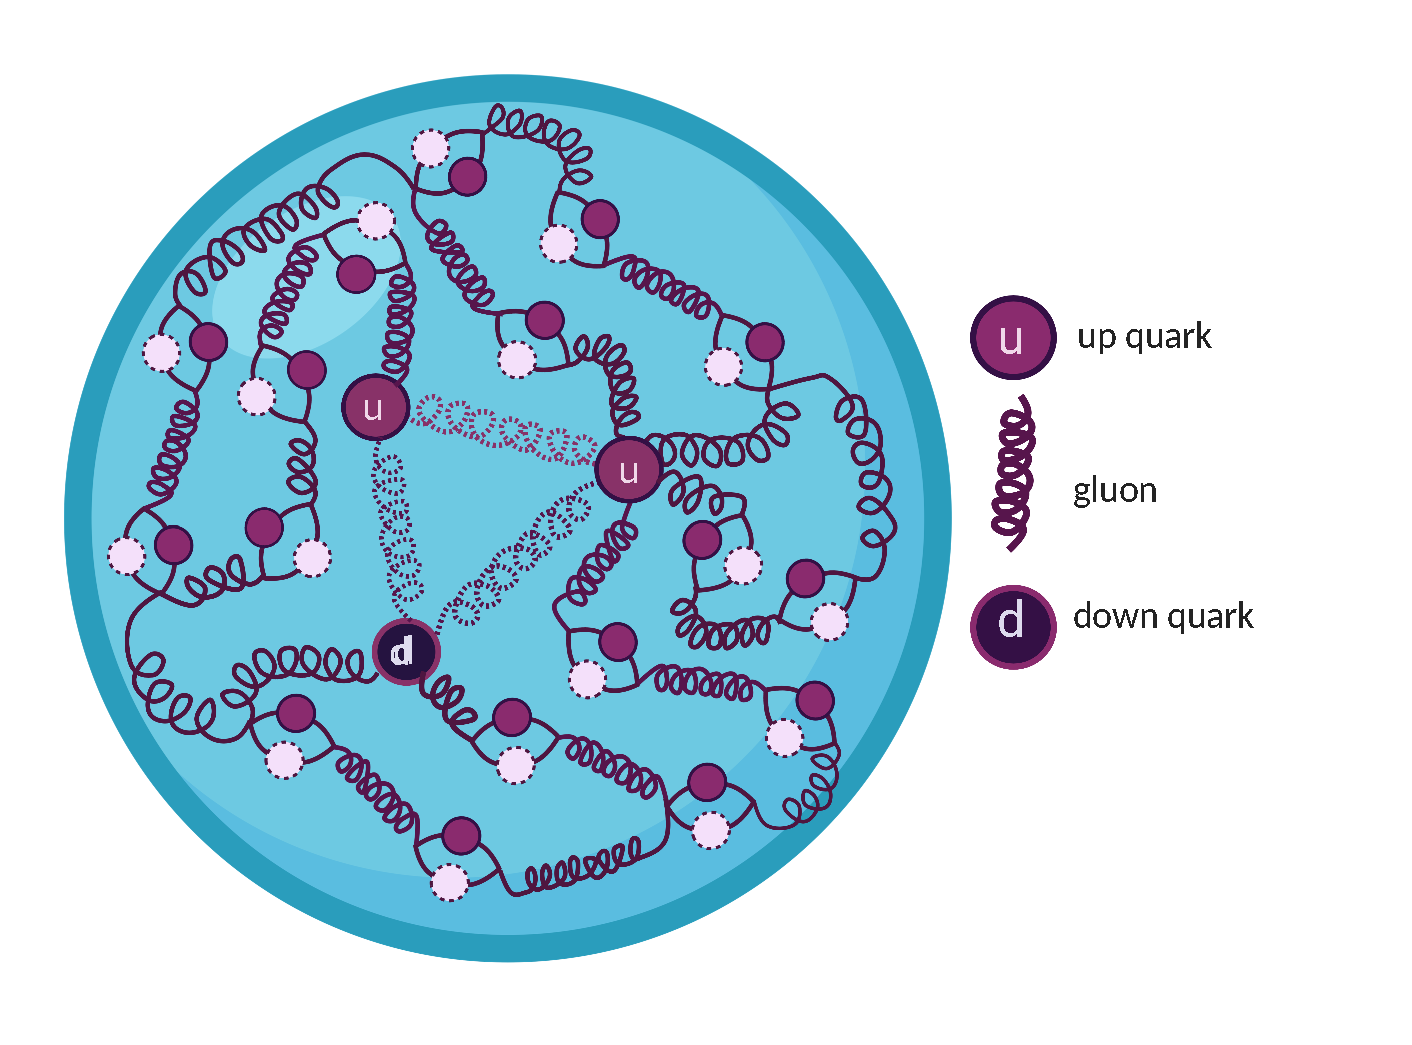
\includegraphics[width=0.6\textwidth]{proton.pdf}
\caption{A visualisation of the internal structure of the proton. Quarks are bound together by gluons.}
\end{figure}

The Standard Model of particle physics has proven thus
far to be an extremely accurate  model of nature at the subatomic scale, and the current focus is on providing ever more precise
experimental and theoretical results to test it and search for new physics which it cannot explain.

Cutting edge high energy physics experiments are currently being carried out at colliders such as the Large Hadron Collider
(LHC) at CERN, and there are many plans for new colliders such as the FCC, ILC and CLIC. Many of these experiments involve the collision of protons. At a basic level we can think of
a proton as being composed of two up quarks and one down quark ($uud$), bound together by the strong
interaction. However, the proton (Fig. \ref{fig:proton}) is in reality
highly complicated and inaccessible to the normal perturbative calculations of Quantum Field Theory (QFT), and can only be treated using probabilistic methods. 

When two protons collide we do not know which constituents,
or ``partons" are interacting, or what individual properties they have, such as their momentum and spin. We need
some way of relating the known properties of the proton to the unknown properties of the partons.
One way of doing this is using parton distribution functions (PDFs), which to first approximation give the
probability of picking out a certain type of parton with certain properties.

Confinement of the quarks means experimental data is collected at the hadronic level, whereas theoretical predictions using QFT are made at the partonic level. The parton model provides a
link between the two; in this framework partonic predictions
are convolved with corresponding PDFs, summing over all possible partonic interactions. This produces PDF-dependent
hadronic predictions. For useful theoretical predictions we therefore need as precise and accurate a handle on the PDFs as possible.

PDFs are unknowns in perturbative Quantum Chromodynamics (QCD), the theory of
the strong interaction. Crucially, they are process independent. This means that
they can be determined in a global fit between a wealth of experimental data and
theoretical predictions. Once constrained, they can then be applied to any process. Fig. \ref{fig:pdfs} shows the fitted functional form of the PDFs.
\begin{figure}[H]
\centering
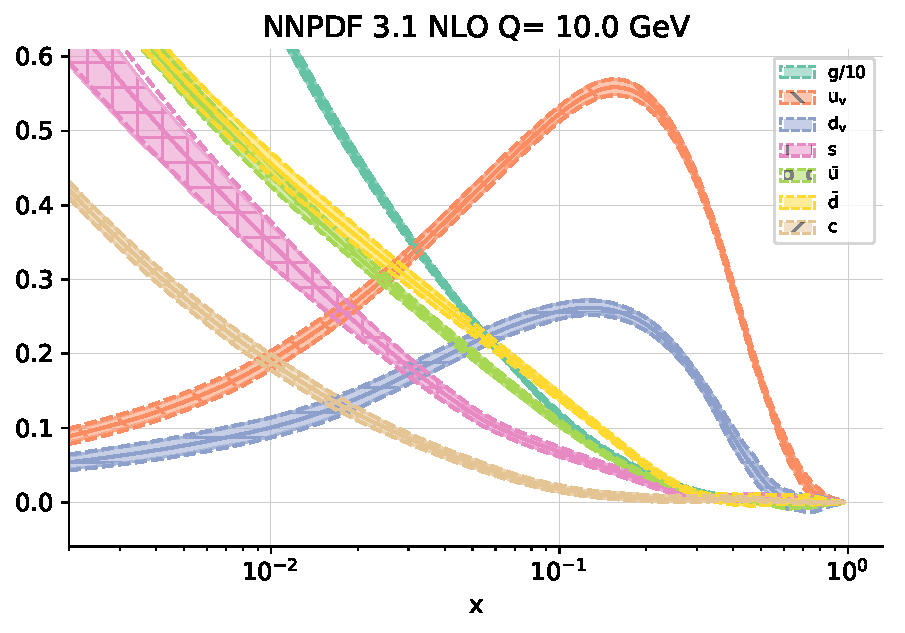
\includegraphics[width=\textwidth]{pdfflavourplot.pdf}
\label{fig:pdfs}
\caption{The different PDF flavours determined in the latest NNPDF3.1 release \cite{Ball:2017nwa}.}
\end{figure}

Any uncertainties in PDF determination will propagate through to future predictions. There are three
places these uncertainties can be introduced:
\begin{enumerate}
\item experimental uncertainties;
\item theory uncertainties;
\item methodological uncertainties (errors from the fitting procedure).
\end{enumerate}
Until recently, experimental uncertainties were the dominant source of error, meaning that theory uncertainties have been largely ignored in standard PDF fits.
However, with the onset of increasingly high precision experiments, a proper treatment of theoretical uncertainties is becoming pressing.

%------------------------------------------------
% Include main matter here
\mainmatter
\eighteenptleading
\chapter{Background}

Parton distribution functions (PDFs) bridge the gap between short and long range physics, allowing perturbative Quantum Chromodynamics (QCD) to be applied at the hadronic scale. They embody the incalculable strongly coupled dynamics, and are determined by a comparison of perturbative theory with experiment. Once determined, their form is process-independent and so they can be re-deployed in future calculations. 

This section provides some background to PDFs neccesary for understanding the remainder of this thesis. It is divided in to two main parts, being the necessary physics and the necessary methodology of PDF determination.

To review the physics, we begin by looking at the process of deep inelastic scattering (DIS), and how the na\"ive parton model was developed to explain these experimental observations. Next we look at this in the context of QCD, see how PDFs fit into the picture, and how they evolve with the scale of the physics. Finally we briefly touch on hadron-hadron collisions, which along with DIS constitute the bulk of the processes in modern PDF fits.

To review the methodology we consider the NNPDF fitting strategy, explaining how theory and experiment are used together with neural networks to determine PDFs.

\subsection{Deep inelastic scattering}
For a more in-depth analysis, see Refs. \cite{pinkbook, hm}. In the following background sections we rely heavily on Ref. \cite{nikhefnotes}.

The notion of bombarding matter to uncover its structure has led to many important discoveries in the last hundred or so years, starting with the Geiger-Marsen experiments from 1908-1913 and the subsequent discovery of the atomic nucleus \cite{nucleus}. In the decades following the discovery of the neutron in 1932, nuclei were probed at higher energies, leading to them being understood in terms of ``form factors" which parametrised their electric and magnetic distributions. At this stage it was clear that they were not point-like particles and so a series of important experiments were carried out in the 1960s at the Standford Linear Accelerator (SLAC), involving a high energy beam of charged leptons scattering off a stationary hadronic target. This process is known as Deep Inelastic Scattering (DIS). 

In this section we will consider the example of electrons incident on protons, as shown in Fig. \ref{fig:dis}. In the deep inelastic regime, there is a large momentum transfer, $q=k-k'$, mediated by a virtual photon. The proton, $P$, with initial momentum $p$, fragments into some hadronic state $X$, and the electron starts with energy $E$ and momentum $k$ and ends with energy $E'$ and momentum $k'$. The momentum transfer is large enough that the masses of the proton and electron can be neglected. 

\begin{figure}[H]
\centering
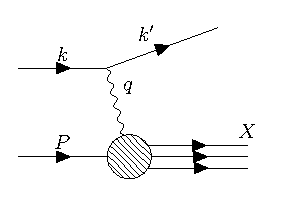
\includegraphics[width=0.7\textwidth]{../diagrams/disdiag.pdf}
\label{fig:dis}
\caption{Deep inelastic scattering}
\end{figure}

It is customary to define some useful variables for help in the analysis, listed in the table below.
\begin{table}[H]
\centering
\begin{tabular}{l|l|l}
  Variable & Definition & Interpretation   \\
 \hline
  $Q^2$ & $- q^2 = -(k-k')^2$   & momentum transfer    \\
  $\nu$ & $p \cdot q = M(E'-E)$ & energy transfer  \\
  $x$   & $\frac{Q^2}{2\nu}$    & scaling parameter \\
  $y$   & $\frac{q \cdot p}{k \cdot p} = 1 - \frac{E'}{E}$ & inelasticity $\in [0,1]$
\end{tabular}
\end{table}
The interaction is made up of a leptonic current (that of the electron) and a hadronic current (the fragmentation of the proton from $P$ to $X$). This means we can express the squared matrix element, $|\mathcal{M}|^2,$ as
\be
\label{eqn:matrixelement}
|\mathcal{M}|^2 = \mathcal{N}_1 \frac{\alpha^2}{q^4} L_{\mu\nu} W^{\mu\nu},
\ee
where $L_{\mu\nu}$ is the leptonic part, determined from perturbative Quantum Electrodynamics (QED), and $W^{\mu\nu}$ is the hadronic part, containing the incalculable strongly coupled dynamics. $\alpha$ is the QED coupling constant and $\mathcal{N}_1$ is a normalisation constant.

From QED, for an unpolarised photon beam in the DIS regime we can use the Feynman rules to write
\bdm
\label{eqn:ltensor}
L_{\mu\nu} = \sum_{spins} \bar{u}(k')\gamma_\mu u(k) \bar{u}(k) \gamma_\nu u(k')
=  Tr \big(\slashed{k'}\gamma_\mu \slashed{k} \gamma_\nu \big)
= \mathcal{N}_2 \bigg( k_\mu k'_\nu + k_\nu k'_\mu -g_{\mu\nu} k\cdot k' \bigg)
= \mathcal{N}_2 \bigg(4 k_\mu k_\nu - 2k_\mu q_\nu - 2 k_\nu q_\mu + g_{\mu \nu} q^2\bigg),
\edm
where in the last line we used the fact that the electron is massless so $
0 = k^{'2} = q^2 + k^2 - 2 q \cdot k \implies q^2 = 2 q \cdot k.$ We have also introduced another constant, $\mathcal{N}_2$.

Finding the hadronic tensor is more difficult because we lack knowledge of the hadronic states $P$ and $X$, so our only constraints are that $W^{\mu\nu}$ is Lorentz-invariant and that the electromagnetic current must be conserved, so $q \cdot W =0$. This allows us to write its general form as
\bdm
\label{eqn:htensor}
W^{\mu\nu}(p,q) = - \bigg(g^{\mu\nu} - \frac{q^\mu q^\nu}{q^2}\bigg) W_1(p,q)
+ \bigg(p^\mu - q^\mu \frac{p \cdot q}{q^2}\bigg) \bigg(p^\nu  - q^\nu \frac{p \cdot q}{q^2} \bigg) W_2 (p, q),
\edm
where $W_1$ and $W_2$ are scalar functions which encapsulate the strong dynamics. These scalar functions are often written as:
\begin{equation}
\begin{split}
F_1(x,Q^2) &= W_1(p,q); \\
F_2(x,Q^2) &= \nu W_2(p,q); \\
F_L(x,Q^2) &= F_2(x,Q^2) - 2x F_1(x,Q^2),
\end{split}
\end{equation}
and are known as the ``structure functions". Often the hadronic tensor is parametrised in terms of $F_2$ and $F_L$, the latter of which is the longitudinal structure function and encapsulates the longitudinal component. 

We can now combine Eqns. \ref{eqn:ltensor} and \ref{eqn:htensor} in Eqn. \ref{eqn:matrixelement}, making use of the fact that due to current conservation $q^\mu L_{\mu \nu} = 0$ to help simplify things. This leads us to the result:
\bdm
\label{eqn:disamplitude}
|\mathcal{M}|^2 = \mathcal{N}_1\mathcal{N}_2^2 \frac{\alpha^2}{q^4} \bigg\{ (-2q^2)W_1(p,q) + \bigg( 4(p \cdot k)^2 - 4 (p \cdot q)(p \cdot k)) \bigg)W_2(p,q) \bigg\}.
\edm

\subsection{The parton model}
Carrying out DIS experiments allows us to measure the structure functions for different values of $x$ and $Q^2$. It transpired that no clear $Q^2$ dependence was observed, and this is known as Bj\"orken scaling \cite{Callan:1973pu}. Because $Q^2$ is the photon's squared momentum, it corresponds to the energy at which the hadron is being probed. The fact that the structure functions are not dependent on this suggests that the interaction is point-like. This led to the formulation of the ``parton model", which described the proton as a composite state made up of point-like particles termed ``partons"\cite{Feynman:1969wa, Feynman:1969ej, Feynman:1973xc}. 

Furthermore, $F_L(x)$ was measured to be 0, known as the Callan-Gross relation \ref{Callan:1968zza, Callan:1973pu}, which suggests that the point-like particles could not absorb longitudinal photons. This fitted in nicely with the quark models developed shortly before \cite{GellMann:1962xb, GellMann:1964nj, Zweig:1964jf, Dothan:1965aa}, which described hadrons in terms of spin-1/2 quarks; spin-1/2 particles cannot interact with longitudinal photons. This was the first experimental evidence for the existence of quarks.

In the DIS regime, $Q^2$ is large and so the virtual photon probes at the short timescale $1/Q$, meaning that the interaction will be effectively instantaneous when compared with the inner proton dynamics which operate at the QCD scale $1/\lambda_{QCD} \sim $ 1 fm.  In the parton model we make the assumption that the partons have only a small momentum transverse to the proton's, and that they are effectively on shell for the interaction ($k^2 \approx 0$). In addition, we consider the process in the infinite momentum frame of the proton, in which it is Lorentz contracted by $M/P$ (a small number), so we can assume the photon will only interact with one parton because it will only traverse a narrow cross-section of the proton. The updated picture is shown in Fig. \ref{fig:disparton}.
\begin{figure}[H]
\centering
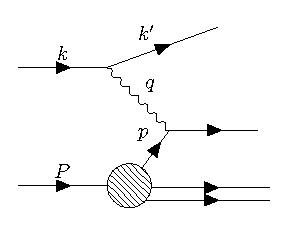
\includegraphics[width=0.7\textwidth]{../diagrams/parton_dis.pdf}
\label{fig:disparton}
\caption{DIS in the parton model. One parton with momentum $p$ interacts with the virtual photon, and the other partons ``spectate".}
\end{figure}

We parametrise the momentum of the interacting parton as $\xi p$, $\xi \in [0,1]$. The parton in the final state has negligible mass so its momentum squared is zero:
\be
\begin{split}
(\xi p+q)^2 &= 0  \\
\implies 2 \xi p \cdot q + q^2 &= 0 \\
\implies 2 \xi p \cdot q - Q^2 &= 0  \\
\implies \xi &= \frac{Q^2}{2p \cdot q} \equiv x.
\end{split}
\ee
This allows us to identify the parton's momentum fraction in this frame with the Bj\"orken $x$ variable.

We can think of the total collection of interactions in terms of a weighted sum over the interactions between the photon and the individual point-like partons, and so can write the proton-level hadronic tensor, $W_{\mu\nu}$ in terms of the parton-level ones, $\hat{W}^q_{\mu\nu}$, as
\be
W_{\mu\nu} = \sum_q  f_q(x) \hat{W}^q_{\mu\nu} \delta(Q^2 - 2xp \cdot q)
= \frac{1}{Q^2} \sum_q  f_q(x) \hat{W}^q_{\mu\nu} \delta(1 - \frac{2xp \cdot q}{Q^2}),
\ee
where $q$ runs over the possible quark flavours and $f_q$ are distributions, with $f_q(x)dx$ giving the probability that in an interaction a parton of flavour $q$ will be found in the momentum range $x \to x +dx$. We call these functions ``parton distribution functions" (PDFs). The delta function appears due to integration over the final phase space of X, and enforces conservation of momentum. Using Eqn \ref{eqn:matrixelement}, we can see that
\be
\label{eqn:ampcomparison}
|\mathcal{M}|^2 = \frac{1}{Q^2} \sum_q  f_q(x) |\mathcal{\hat{M}}_q|^2.
\ee
This means that the total amplitude can be expressed in terms of the partonic amplitudes and the PDFs. If we assume that the partons are massless Dirac particles, we can infer the partonic amplitudes directly from that of electron-muon scattering. In this scenario the electron has a current like Eqn. \ref{eqn:ltensor}, and the muon has the same, but with the substitutions $k \to p$ and $q \to -q$. Once again we can use $q_\mu L^{\mu \nu} =0$ and the expression
\be
|\mathcal{M}_{(e \mu)}|^2 = \mathcal{N}_1 \frac{\alpha^2}{q^4} L^{(e)}_{\mu\nu} L_{(\mu)}^{\mu\nu}
\ee
to show (in the massless limit)
\be 
|\mathcal{M}_{(e \mu)}|^2 = \mathcal{N}_1\mathcal{N}_2^2 \frac{\alpha^2}{q^4} \bigg( 16 (p \cdot k)^2 + 8 q^2 (p \cdot k) + 2 q^4 \bigg).
\ee
Using the symmetry of Fig. \ref{fig:disparton}, we can see this is analogous to $|\mathcal{\hat{M}}_q|^2$ under the substitution $p \to xp$, provided we replace the charge of the electron, $e$, with that of the parton, $e_q$, so that $\alpha \to e_q \alpha$. Making use of the expression $p \cdot k = Q^2/2xy$,
\be 
\begin{split}
|\mathcal{\hat{M}}_q|^2 &= \mathcal{N}_1\mathcal{N}_2^2 \frac{e_q^2 \alpha^2}{q^4} \bigg\{ 4 (2xp \cdot k)^2 + 4 (2 x p\cdot k) q^2 + 2q^4 \bigg\} \\
&= \mathcal{N}_1\mathcal{N}_2^2 \frac{e_q^2 \alpha^2}{Q^4} \bigg\{ 4 \bigg(\frac{Q^2}{y}\bigg)^2 - 4 \bigg(\frac{Q^2}{y}\bigg) Q^2 + 2Q^4 \bigg\} \\ 
&= \mathcal{N}_1\mathcal{N}_2^2 e_q^2 \alpha^2 \bigg\{ 2 + 4 \bigg( \frac{1-y}{y^2} \bigg) \bigg\}.
\end{split}
\ee 
Now we can use this alongside Eqn. \ref{eqn:disamplitude} in  Eqn. \ref{eqn:ampcomparison}, giving us
\be 
\begin{split}
F_1 &\equiv W_1 = \sum_q f_q(x)e_q^2, \\
F_2 &\equiv \nu W_2 = 2x \sum_q f_q(x) e_q^2.
\end{split}
\ee
We see immediately that the Callan-Gross relation, $F_L(x) \equiv F_2(x) - 2x F_1(x) = 0$, is satisfied, as was observed experimentally.

However, it was soon observed that this relation only held in the limit $Q^2 \to \infty$, and that at smaller scales there were so-called ``scaling violations". In order to understand this behaviour it is necessary to revisit the parton model in the light of Quantum Chromodynamics (QCD).

\subsection{Quantum Chromodynamics (QCD)}
QCD is the theory of the strong force. This is responsible for binding together hadrons, and explains the short-range interactions which occur within them. It is a gauge theory where the quark fields are realised as fundamental representations of the $SU(3)$ symmetry group and interactions between them are carried out via gauge bosons termed ``gluons", which are expressed in the adjoint representation \cite{grinstein2006introductory}. 

Quark models showed that the structure of observed hadrons can be explained using the $SU(3)_f$ group alongside the association of quarks with different ``flavours"  \cite{GellMann:1962xb, GellMann:1964nj, Zweig:1964jf, Dothan:1965aa} . The additional $SU(3)_c$ colour symmetry was put forwards in order that the quarks satisfied Fermi-Dirac statistics \cite{Greenberg:1964pe}. Each quark is assigned an additional colour ((anti-)red, green or blue) in such a way that the composite hadrons are colourless. The additional local symmetry is accompanied by eight gauge bosons, the gluons. Colour is the charge of QCD, just as electric charge is for QED. An important difference is that, unlike chargeless photons in QED, the gluons themselves also have colour and this leads to complex self-interactions. 


QCD can be expressed through the Lagrangian
\be
\mathcal{L} = -\frac{1}{4}F_{\mu \nu}^a F^{a \mu \nu} + \bar{q}^i(i \slashed{\mathcal{D}}_i^j - m \delta_i^j) q_j,
\ee
where the covariant derivative is
\be 
\mathcal{D}_\mu \psi(x) = (\partial_\mu -i\sqrt{4 \pi \alpha_s}T^a A_\mu^a) \psi(x) ,
\ee
and the field strength tensor is
\be 
F^a_{\mu \nu} = \partial_\mu A_\nu^a - \partial_\nu A_\mu^a + \sqrt{4 \pi \alpha_s} f^{abc} A_\mu^b A_\nu^c.
\ee
The indices $\mu, \nu$ are spacetime indices, $i, j$ are quark colour indices and $a,b, c$ are gluon colour indices. The first term in the Lagrangian arises from the self-interacting gluons, $A$, and the second term from the quarks, $q$, which obey the Dirac equation. $\alpha_s$ is the strong coupling constant, which dictates the strength of the interaction, and $T^a$ are the eight $SU(3)$ generators. $f^{abc}$ are the SU(3) structure constants. For simplicity we have assumed all quarks have the same mass, $m$. Note that gauge fixing and ghost terms are omitted. For more information see Ref. \cite{pinkbook}.

Colour self-interactions give rise to the important properties of ``confinement" and ``asymptotic freedom". The QCD potential is of the form
\be 
V(r) \sim \frac{\alpha}{r} + kr,
\ee
where the first term drops off with distance like QED, but the second term comes from the self-interactions and means that separating two quarks takes infinite energy. This explains why we have not observed free quarks (``confinement"). Additionally, the QCD colour charge decreases with shorter distances. This means that at very short distances or high energies the quarks become ``free", which is known as ``asymptotic freedom". This crucial fact allows us to applythe tool of perturbation theory in such regimes. 

QCD is subject to divergences in the ultra-violet (high energies) and infra-red (low energies). The former are regulated by renormalisation, which introduces a ``renormalisation scale", $\mu_R$. This is non-physical, and so observables cannot depend on it. This observation leads to a ``renormalisation group equation" (RGE), which can be solved by the introduction of a running coupling, dependent on the scale $Q^2$ (i.e. $\alpha_s \to \alpha_s(Q^2)$), which satisfies
\be
\label{eqn:rge}
Q^2 \frac{\partial \alpha_s}{\partial Q^2} = \beta (\alpha_s),
\ee
The beta function, $\beta(\alpha_s)$, can be expressed perturbatively as an expansion in $\alpha_s$ and is currently known to N$^3$LO.

At one-loop order the solution of this equation is
\be 
\alpha_s(Q^2) = \frac{\alpha_s(\mu_R^2)}{1+ \beta_0 \alpha_s (\mu_R^2) \ln\big(\frac{Q^2}{\mu_R^2}\big)},
\ee
where $\beta_0$ is the first coefficient of the $\beta$ expansion. From this solution we can explicitly see asymptotic freedom because $\alpha_s$ decreases as the energy scale increases. We also see the role of the renormalisation scale in specifying a particular reference value for $\alpha_s$. This solution is not exact because the RGE \ref{eqn:rge} only holds to all orders. Any residual $\mu_R$ dependence characterises the accuracy of our calculation, because going to higher and higher orders should reduce this dependence, eventually to 0.

Quantities are infra-red safe if they do not depend on long-distance physics. This means we can apply perturbation theory because $\alpha_s$ is small enough in the short-distance regime. Unforunately at the partonic level structure functions and cross sections are not infra-red safe. 

\subsection{The QCD improved parton model and factorisation}

In the na\"ive parton model, we did not include any interactions involving gluons; their incorporation leads to the QCD improved parton model. The addition of gluons leads to significant complications, owing to the fact that the interacting quarks are free to emit gluons at some stage before detection (remember the detector is at a long-distance so we cannot ignore the long-distance physics). When these gluons are ``soft" (low energy) or collinear to one of the partons we run into IR divergences. This situation is equivalent to the internal propagator quark going on-shell, or in other words there is a large time separation between the partonic interaction and the gluon emission. The observed violation of Bj\"orken scaling has its origins in interactions with gluons. In IR-safe observables the soft and collinear divergences exactly canel \cite{Kinoshita:1962ur, Lee:1964is}, but for other cases we need a way of dealing with the disparate short- and long- scale physics. 

This is done using the factorisation theorem \ref{Collins:1989gx}, which allows us to factorise the incalculable long-distance physics into the PDFs, meaning we are able to use perturbative QCD as a predictive theory. The PDFs are then non-perturbative, meaning we must obtain them from experiments, but they are universal quantities and so once determined can be applied everywhere, much like the coupling constants. This process introduces the artificial ``factorisation scale", $\mu_F$, in addition to the renormalisation scale. The factorisation scale separates the short- and long- distance physics; loosely, if a parton's transverse momentum is less than $\mu_F$ it is considered part of the hadron and is factored into the PDFs, otherwise it is seen as taking part in the hard scattering process, and will appear in the partonic cross section.

\begin{figure}[H]
\centering
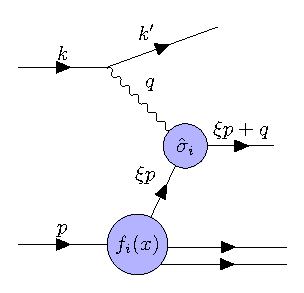
\includegraphics[width=0.7\textwidth]{../diagrams/improvedparton_dis.pdf}
\label{fig:improvedparton}
\caption{Factorisation and the QCD improved parton model}
\end{figure}


We can write a DIS cross section as
\be
\label{eqn:disfact}
\sigma^{DIS} = \sum_i \int dx f_i(x, \mu_F^2) \hat{\sigma}_i \bigg(x, \frac{Q^2}{\mu_F^2} \bigg),
\ee
corresponding to Fig \ref{fig:improvedparton}. 

We can see how this works in practice by considering the case where a quark emits a gluon before interaction with the photon, such as in Fig. \ref{fig:scalingviolation}. Here the parent parton, with fraction $y$ of the proton's momentum, emits a gluon giving rise to a daughter parton with a fraction $z$ of the parent hadron's momentum. We can see that $z = x/y$.

\begin{figure}[H]
\centering
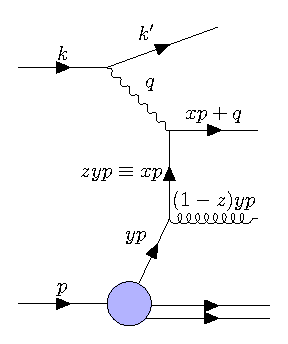
\includegraphics[width=0.7\textwidth]{../diagrams/scalingviolation.pdf}
\label{fig:scalingviolation}
\caption{A quark radiating a gluon before interacting.}
\end{figure}

It transpires (see Ref. \cite{hm} for the derivation) that the structure function $F_2$ can be expressed as
\begin{dmath}
\label{eqn:stfn}
\frac{F_2(x,Q^2)}{x} = \sum_i e_i^2 \int_x^1 \frac{dy}{y} f_i(y) \bigg[ \delta \bigg( 1- \frac{x}{y} \bigg) + \frac{\alpha_s}{2 \pi} \mathcal{P}_{qq} \bigg( \frac{x}{y} \bigg) \ln \bigg( \frac{Q^2}{m^2} \bigg) \bigg].
\end{dmath}
$m$ is a cutoff introduced to regularise the collinear divergence and you can see that as $m \to 0$ the structure function diverges. A divergence also occurs for $(1-z) \to 0$, and this is a soft divergence because it corresponds to the gluon being emitted with zero momentum. The quantity $\mathcal{P}_{qq}$ is the quark-quark ``splitting function", detailing the probability that a quark emits a gluon leaving a daughter quark with fraction $z$ of the parent's momentum. In the $\overline{MS}$ renormalisation scheme this has the form
\be 
\mathcal{P}_{qq} = \frac{4}{3} \bigg( \frac{1+z^2}{1-z} \bigg).
\ee
We want an expression which is free from the soft and collinear divergences. We can proceed by defining
\be 
\mathcal{I}^i_{qq}(x) \equiv \frac{\alpha_s}{2 \pi} \int_x^1 \frac{dy}{y} f_i(y)\mathcal{P}_{qq} \bigg( \frac{x}{y} \bigg),
\ee
and separating \ref{eq:stfn} into a singular part and a calculable part, like
\begin{dmath}
\frac{F_2(x,Q^2)}{x} = \sum_i e_i^2 \bigg[ f_i(x) + \mathcal{I}^i_{qq}(x)  \ln \bigg( \frac{\mu_F^2}{m^2} \bigg) + \mathcal{I}^i_{qq}(x)  \ln \bigg( \frac{Q^2}{\mu_F^2} \bigg) \bigg].
\end{dmath}
Notice we introduced the artificial factorisation scale, $\mu_F$, to do this. Grouping the singular terms together as
\be
f_i(x, \mu_F^2) =  f_i(x) + \mathcal{I}^i_{qq}(x)  \ln \bigg( \frac{\mu_F^2}{m^2} \bigg),
\ee
we have factorised the divergences into the PDF $f_i(x)$, giving a new PDF, $f_i(x, \mu_F^2)$ , which also depends on $\mu_F$.
and noting that at leading order $f_i(y) = f_i(y, \mu_F^2)$, we are able to write
\begin{dmath}
\frac{F_2(x,Q^2)}{x} = \sum_i e_i^2 \bigg[ f_i(x, \mu_F^2) + \frac{\alpha_s}{2 \pi} \int_x^1 \frac{dy}{y} f_i(y, \mu_F^2)\mathcal{P}_{qq} \bigg( \frac{x}{y} \bigg) \ln \bigg( \frac{Q^2}{\mu_F^2} \bigg) \bigg]+ \mathcal{O}(\alpha_s^2).
\end{dmath}
We know that $F_2$ is an observable quantity and thus should be independent of $\mu_F$, leading to a RGE:
\be
\begin{split}
\frac{1}{e_i^2x} \frac{\partial F_2(x,Q^2)}{\partial \ln \mu_F^2} &= \frac{\partial f_i(x,\mu_F^2)}{\partial \ln \mu_F^2} \\ &+ \frac{\alpha_s}{2 \pi} \int_x^1 \frac{dy}{y} \bigg( \frac{\partial f_i(y,\mu_F^2)}{\partial \ln \mu_F^2}\ln \bigg( \frac{Q^2}{\mu_F^2} \bigg) -  f_i(y, \mu_F^2) \bigg)\mathcal{P}_{qq} \bigg( \frac{x}{y} \bigg)\\ &= 0.
\end{split}
\ee
This can be further simplified by noting that $\frac{\partial f_i(y,\mu_F^2)}{\partial \ln \mu_F^2}$ is of $\mathcal{O}(\alpha_s^2)$, and so
\be
\frac{\partial f_i(x,\mu_F^2)}{\partial \ln \mu_F^2}  =  \frac{\alpha_s}{2 \pi} \int_x^1 \frac{dy}{y} f_i(y, \mu_F^2)\mathcal{P}_{qq} \bigg( \frac{x}{y} \bigg).
\ee
This equation describes the evolution of the newly defined PDFs with scale, a product of the factorisation of the divergences into them. In practice this equation is solved numerically. 

When we also include the gluon as a parton, we open ourselves up to more splitting possibilities (e.g. gluon $\to$ quark and gluon $\to$ gluon), and this result generalises to a set of coupled differential equations known as the DGLAP equations~\cite{jr:altarelli, jr:dokshitzer,jr:gribov}:
\be 
\label{eqn:DGLAP}
\frac{\partial f_i}{ \partial \ln \mu_F^2} = \sum_i \frac{\alpha_s}{2 \pi} \mathcal{P}_{ij} \otimes f_j,
\ee
where we have used the Mellin convolution, defined
\be 
\mathcal{P} \otimes f \equiv \int_x^1 \frac{dy}{y} \mathcal{P} \bigg( \frac{x}{y} \bigg)f(y, \mu_F^2),
\ee
and the index $i$ runs from $-n_f$ to $n_f$ (where $n_f$ is the number of flavours), with the negative indices referring to the antiquarks, 0 to the gluon and the positive ones to the quarks.

\subsection{Hadroproduction}

At the LHC most processes involve the interaction of two protons. Hadron-hadron collisions can be approached in much the same way as DIS, but instead the process is like in Fig. \ref{fig:hadroproduction}. Because two protons are involved the expression for the cross section is the natural extension of the DIS case (\ref{eq:disfact}):
\be
\sigma = \sum_{i,j} \int dx_1 dx_2 f_i(x_1, \mu_F^2) f_j(x_2, \mu_F^2) \hat{\sigma}_{ij}\bigg(x_1, x_2, \frac{Q^2}{\mu_F^2},...\bigg).
\ee

\begin{figure}[H]
\centering
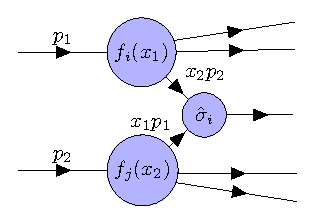
\includegraphics[width=0.7\textwidth]{../diagrams/hadroproduction.pdf}
\label{fig:hadroproduction}
\caption{Factorisation in hadron-hadron collisions.}
\end{figure}

Write about higher order corrections and factorisation!

\subsection{Sum rules}

Although PDFs may seem at first sight to be totally unknown there are some theoretical observations which
we can use to constrain their form.
These are known as the ``sum rules''~\cite{ob:ellis}. Intuitively, adding up all the momenta of the partons must equal the
momentum of the proton. This enforces the condition

\beq
  \int_0^1 dx \sum_i x f_i(x,Q^2) = 1.
\eeq

The other thing we know about the
proton is that it is made up of two up and one down (and no strange)
``valence'' quarks. Any other quarks must be pair-produced from the sea, and
therefore come with an antiquark of the same flavour. So we can normalise the PDFs using the expressions: 

\begin{subequations}
 \beq
   \int_0^1 dx \big( f_u - f_{\bar{u}} \big) = 2;
 \eeq
 \beq
   \int_0^1 dx \big( f_d - f_{\bar{d}} \big) = 1;
 \eeq
 \beq
   \int_0^1 dx \big( f_q - f_{\bar{q}} \big) = 0, \qquad q = s, c, t, b.
 \eeq
\end{subequations}

Note that these conditions require that the PDFs are integrable. 


\section{Determining PDFs}

In this section we review the necessary background for PDF determination within the NNPDF \cite{nnpdf} framework. First we touch on the experimental and theoretical inputs to PDF fits, then we summarise the NNPDF fitting strategy, and finally we detail information on neural networks specific to this context.

\subsection{Experimental and theoretical input}


NNPDF uses a variety of experimental data from a number of particle colliders, including those based at CERN \cite{cern} and Fermilab \cite{fermilab}. These are observables such as cross sections, differential cross sections and structure functions. Fig. \ref{data} is a plot of the $(x,Q^2)$ range spanned by the datasets in the latest NNPDF3.1~\cite{Ball:2017nwa} release. The majority of the data are from DIS processes, which are crucial in determining PDF functional form, but in recent years increasingly more LHC collider data has been added including $t\bar{t}$ production, high energy jets and single top production \cite{Nocera:2019wyk}. For a full review of the data, see Ref. \ref{Ball:2017nwa}.

\begin{figure}
\centering
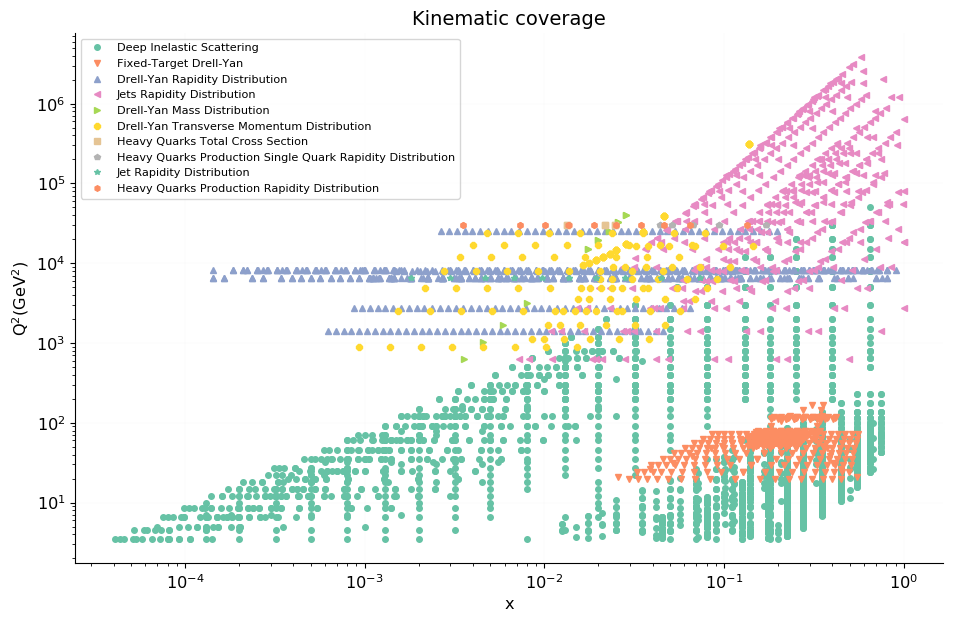
\includegraphics[width=15cm]{background/NNPDF31_nlo_as_0118_1000_markers0_fitcontext_plot_xq2.png}
\caption{Plot of the $(x,Q^2)$ range spanned by data included in the latest NNPDF3.1 NLO fit.}
\label{data}
\end{figure}

Theoretical predictions of the corresponding parton-level observables are computed using external codes such as \texttt{MCFM}~\cite{jr:mcfm}, \texttt{aMC@NLO}~\cite{Alwall:2014hca}, \texttt{DYNNLO}~\cite{Catani:2009sm}, \texttt{FEWZ}~\cite{Gavin:2010az} and \texttt{NLOjet++}~\cite{Catani:1996vz}. These are converted to higher orders of perturbation theory as necessary using QCD and electroweak correction (``$k$'') factors. They are then combined with DGLAP evolution kernels, which evolve PDFs from an initial reference energy scale to the energy scale of each experiment using the DGLAP equations (Eqn. \ref{eqn:DGLAP}). 


\subsection{Experimental uncertainties}
\label{sec:expuncs}

Experimental uncertainties are described using a covaraince matrix, $C_{ij}$, which gives the uncertainties and correlations between each of the data points $i,j = 1,...,N_{dat}$. It encapsulates the total breakdown of errors, $\sigma$, and can be constructed using uncorrelated errors ($\sigma_i^{uncorr}$), and  additive ($\sigma_{i,a}$) and multiplicative  ($\sigma_{i,m}$) correlated systematic errors (more on these below):
\beq
  C_{ij} = \delta_{ij}\sigma_i^{uncorr}\sigma_j^{uncorr} + \sum_a^{add.}\sigma_{i,a}\sigma_{j,a} +
  \bigg( \sum_m^{mult.}\sigma_{i,m}\sigma_{j,m} \bigg) D_i D_j,
\label{eq:expcov}
\eeq
where $D_i$ are the experimental data values.

Structurally, the uncorrelated statistical uncertainties appear down the diagonal and these are what we would recognise intuitively as the statistical error ``on a data point". However, correlated
systematic uncertainties can also appear on the off-diagonals. Correlated uncertaintes include
those which link multiple data points, for example systematic uncertainties from a particular
detector which will affect all of its data in a similar way.

Systematic uncertainties further divide into two types, ``additive'' and ``multiplicative''.
Additive systematics are perhaps a more familiar type of error, and are independent of the
datapoint values themselves. On the other hand,  multiplicative systematics depend on the measured values. In the context of particle physics 
experiments, a common example is total detector luminosity. This is because recorded cross
sections are dependent on the luminosity of the detector; a higher luminosity means more
collisions will take place so the measured cross section will be greater.

Fig. \ref{fig:expcovmat} is an example of an experimental covariance matrix for data included in an NNPDF fit. The data are grouped according to what type of process the interaction belongs to (DIS charged current (CC) and neutral current (NC), Drell-Yan (DY), jets and top production). Systematic correlations within experiments are responsible for off-diagonal contributions, and these are mostly positive correlations but there is some anticorrelated behaviour in DIS CC, as a result of data in different kinematic regimes. 

\begin{figure}
\centering
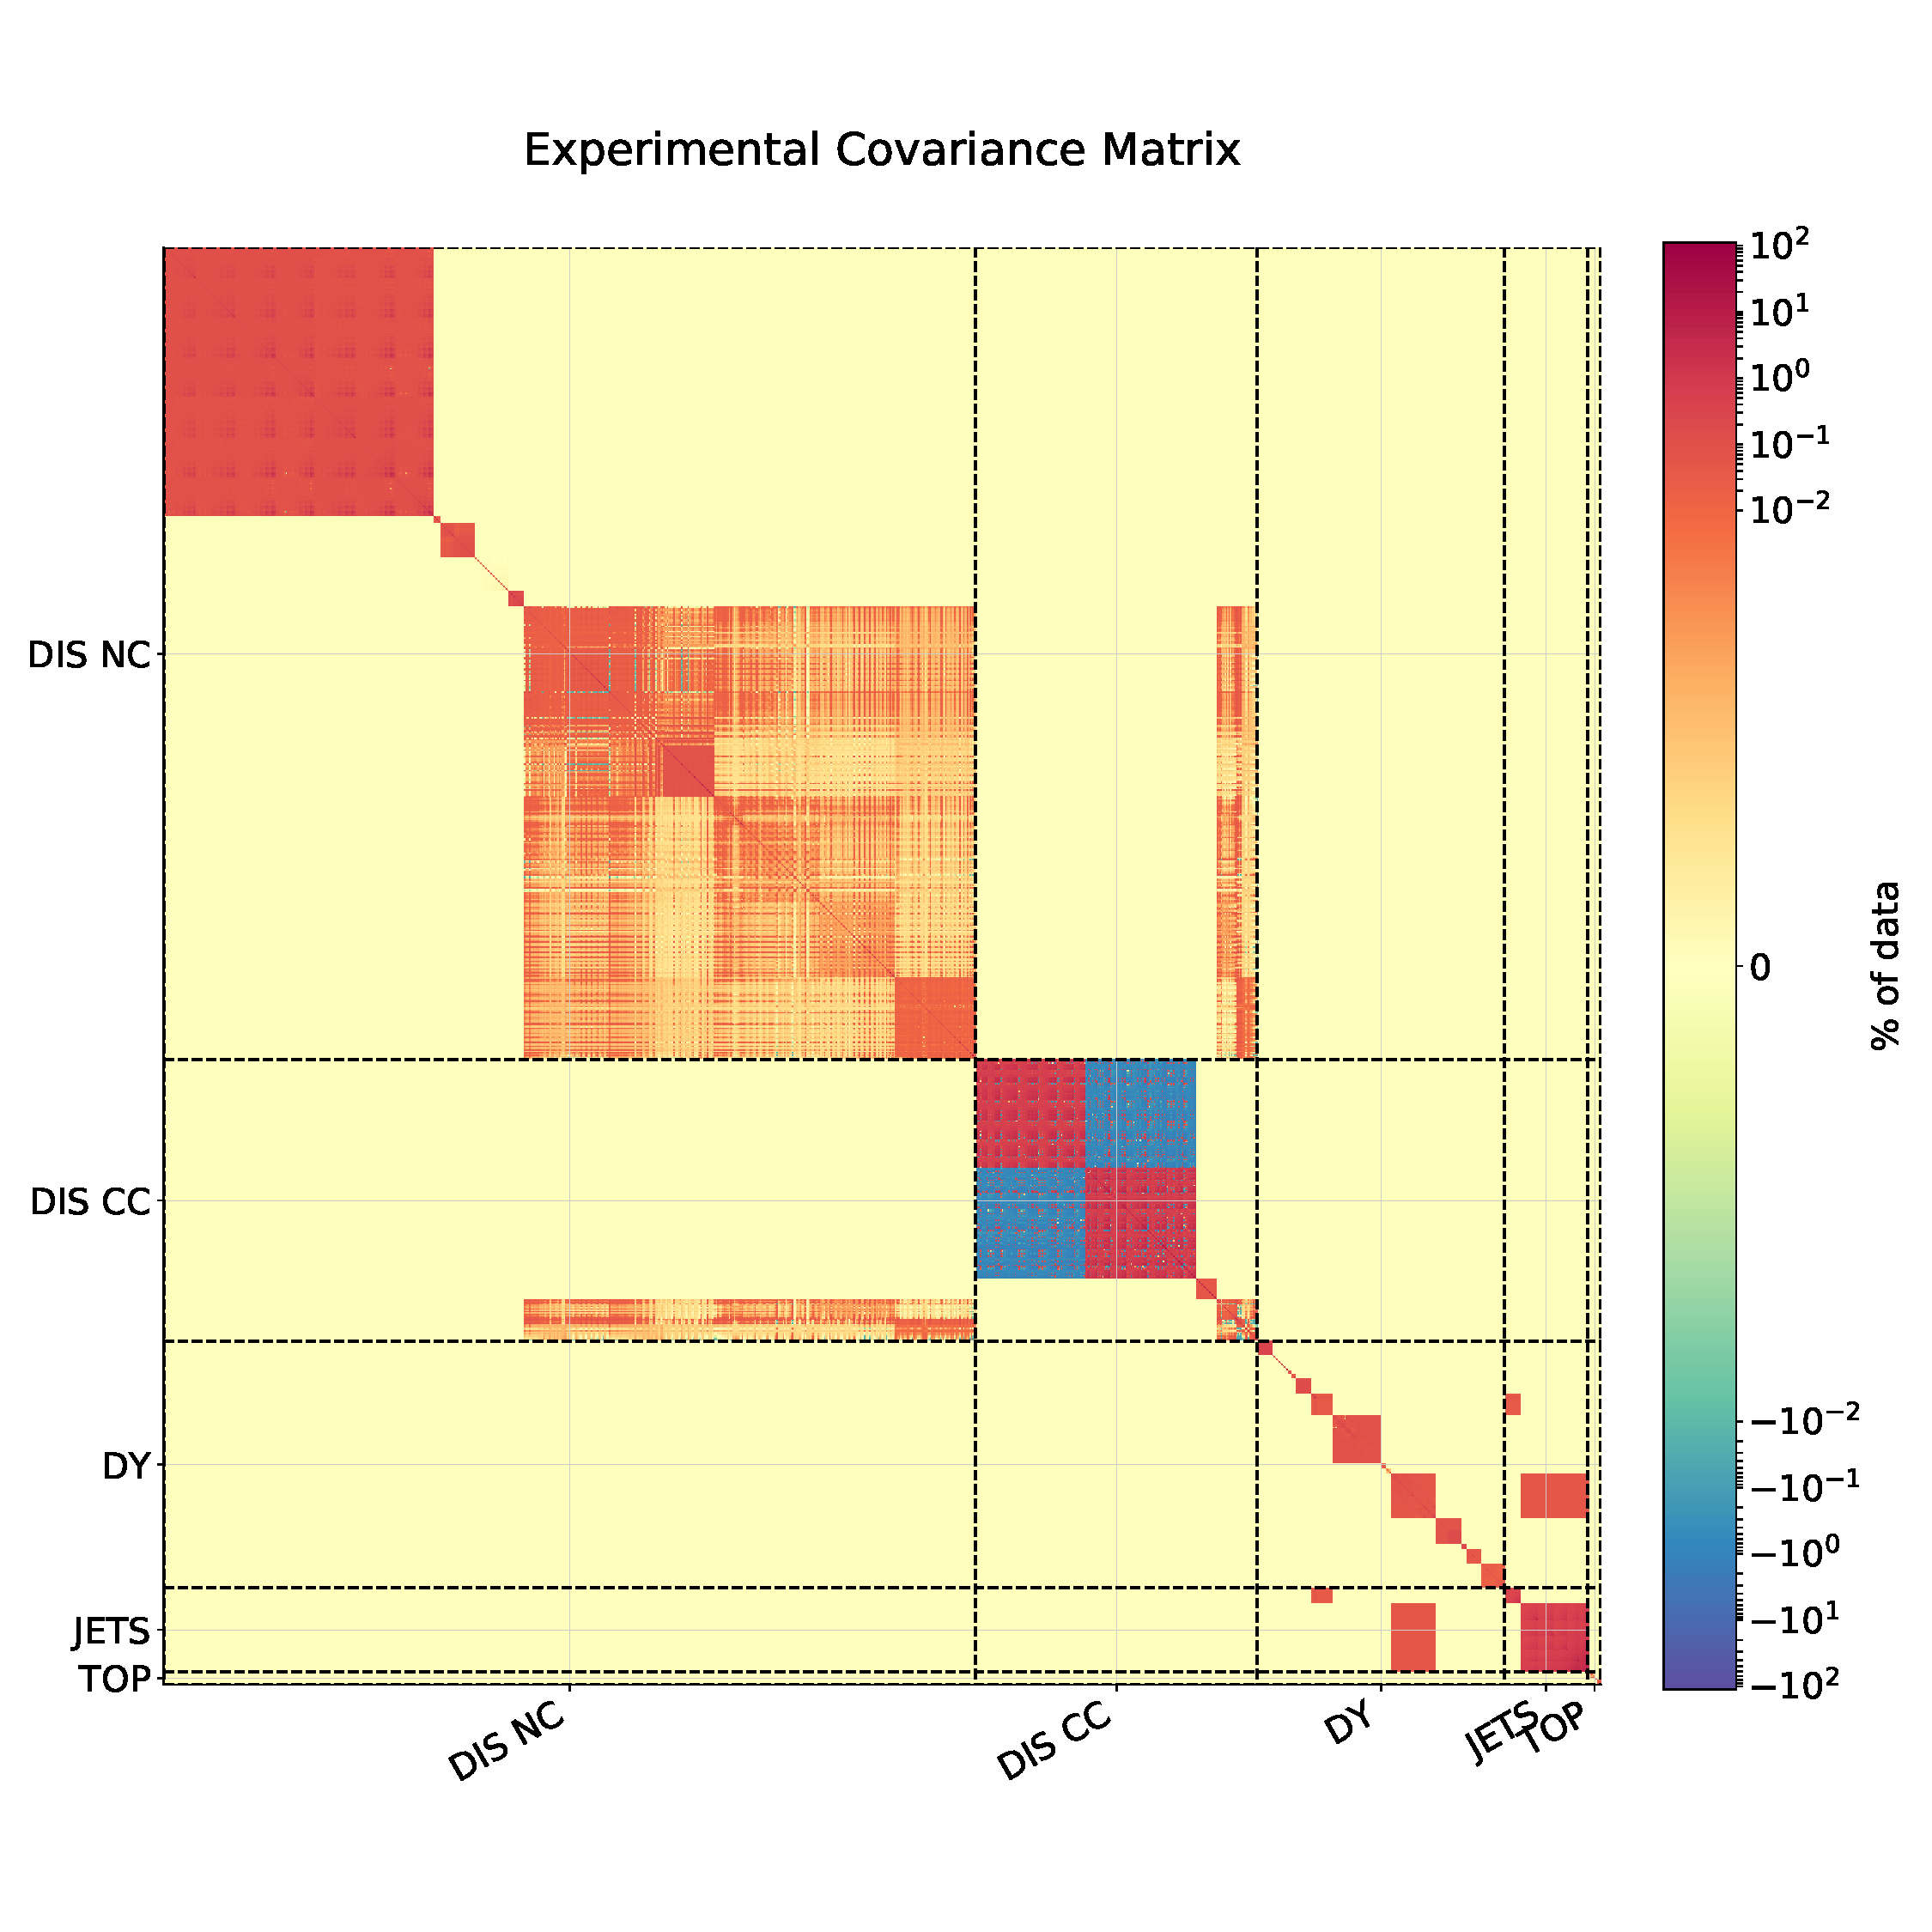
\includegraphics[width=15cm]{background/exp_covmat.pdf}
\caption{An example of an experimental covariance matrix for data included in an NNPDF fit. The data are grouped according to what type of process the interaction belongs to (DIS charged current (CC) and neutral current (NC), Drell-Yan (DY), jets and top production).}
\label{fig:expcovmat}
\end{figure}

The covariance matrix can be used to define the $\chi^2$ figure of merit, 
\be
\label{eqn:chi2}
\chi^2 = \frac{1}{N_{dat}} (D_i-T_i) C_{ij}^{-1} (D_j-T_j),
\ee
which measures the goodness of fit between the experimental data $D_i$ with associated error breakdown $C_{ij}$, and theory predictions $T_i$. In practice, this definition is subject to d'Agostini bias \cite{DAgostini:1993arp} due to the presence of normalisation uncertainties. To avoid this, NNPDF employ the iterative $t0$ procedure \cite{Ball:2009qv} whereby $D_i$ in Eqn. \ref{eqn:expcov} are replaced initially with the predictions from a baseline fit, and the covariance matrix is iterated concurrently with preprocessing. 


\subsection{NNPDF fitting strategy}

There are a number of groups currently active in carrying out PDF fits including MSTW~\cite{Martin:2009bu}, CTEQ~\cite{Dulat:2015mca}, NNPDF~\cite{nnpdf}, HERAPDF/xFitter~\cite{CooperSarkar:2011aa} and ABM~\cite{Alekhin:2013nda}.

The work in this thesis has been carried out in the framework developed by the NNPDF collaboration, so we will concentrate on this fitting strategy. There are two main features which differ from other fitting collaborations'~\cite{Forte:2002fg}. These are:
\begin{enumerate}
\item  The use of Monte Carlo approach to error analysis;
    \item  Fitting using artificial neural networks.
\end{enumerate}

In the following sections we will provide an overview of these aspects, which can be found in more detail in Refs. \cite{Ball:2010de, Ball:2012cx, Ball:2017nwa}.
\subsection{Monte Carlo approach}

The uncertainties in the functional form of PDFs come as a direct consequence of the uncertainties in the experimental and theoretical input. In order to propagate experimental uncertainties through to the PDFs, NNPDF represent the experimental data (central values and uncertainty distribution) as a Monte Carlo ensemble. This is a set of $N_{rep}$ Monte Carlo ``replicas" which, given high enough replica number, have a mean value equal to the data central value and covariance equal to the experimental covariance. Fig. \ref{fig:MC} is a schematic illustrating the generation of these ``pseudodata", $D^{(k)}$, $k=1,...,N_{rep}$.
\begin{figure}
\centering
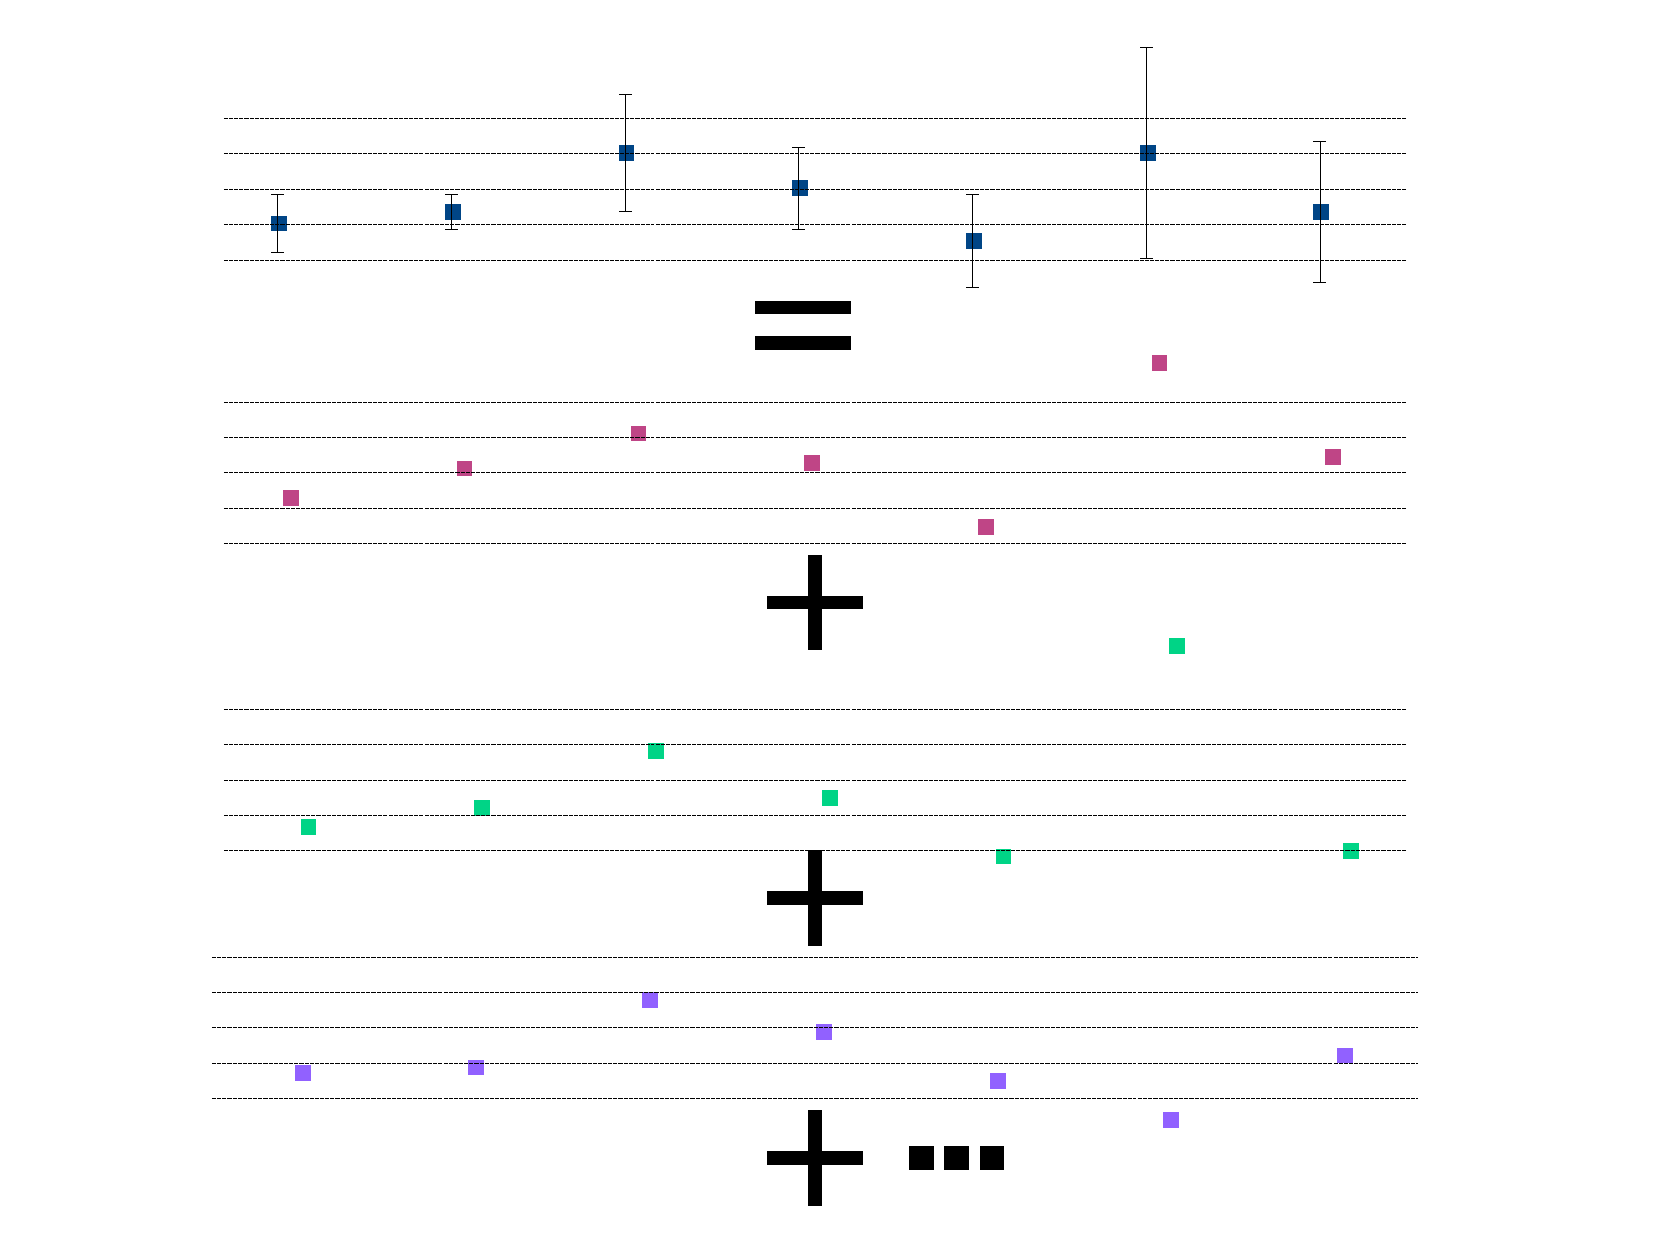
\includegraphics[width=0.7\textwidth]{background/monte_carlo.pdf}
\caption{Schematic of the generation of Monte Carlo replicas of pseudodata from data with uncertainties.}
\label{fig:MC}
\end{figure}
They are generated using Gaussian random numbers $n_a^{(k)}$ and $\hat{n}_p^{(k)}$:
\be
D^{(k)} = (D^0 + \sum_a n_a^{(k)} \sigma^a) \prod_m (1 + \hat{n}_m^{(k)}\sigma^p),
\ee
where $D_0$ is the (symmetrised) experimental data value, and $\sigma^a$ and $\sigma^m$ are the additive and multiplicative uncertainties discussed in Sec. \ref{sec:expuncs}. Explicitly, the pseudodata replicas satisfy the relations:
\be
\langle D_i^{(k)} \rangle = D_i^0; \qquad (\langle  D_i^{(k)} \rangle -D_i^0)(\langle  D_j^{(k)} \rangle-D_j^0) = C_{ij},
\ee
where the notation $\langle \cdot \rangle$ denotes the mean over replicas. Fig. \ref{fig:datarepchorus} shows the distribution of pseudodata for a single data point.

\begin{figure}
\centering
\includegraphics[width=0.7\textwidth]{background/datarepchorus.png}
\caption{Histogram of distribution of 100 pseudodata replicas for a single data point, normalised to $D^0$. The purple line is the mean value $\langle D^{(k)} \rangle$, which is equal to $D^0$ to arbitrary precision.}
\label{fig:datarepchorus}
\end{figure}
\begin{figure}
\centering
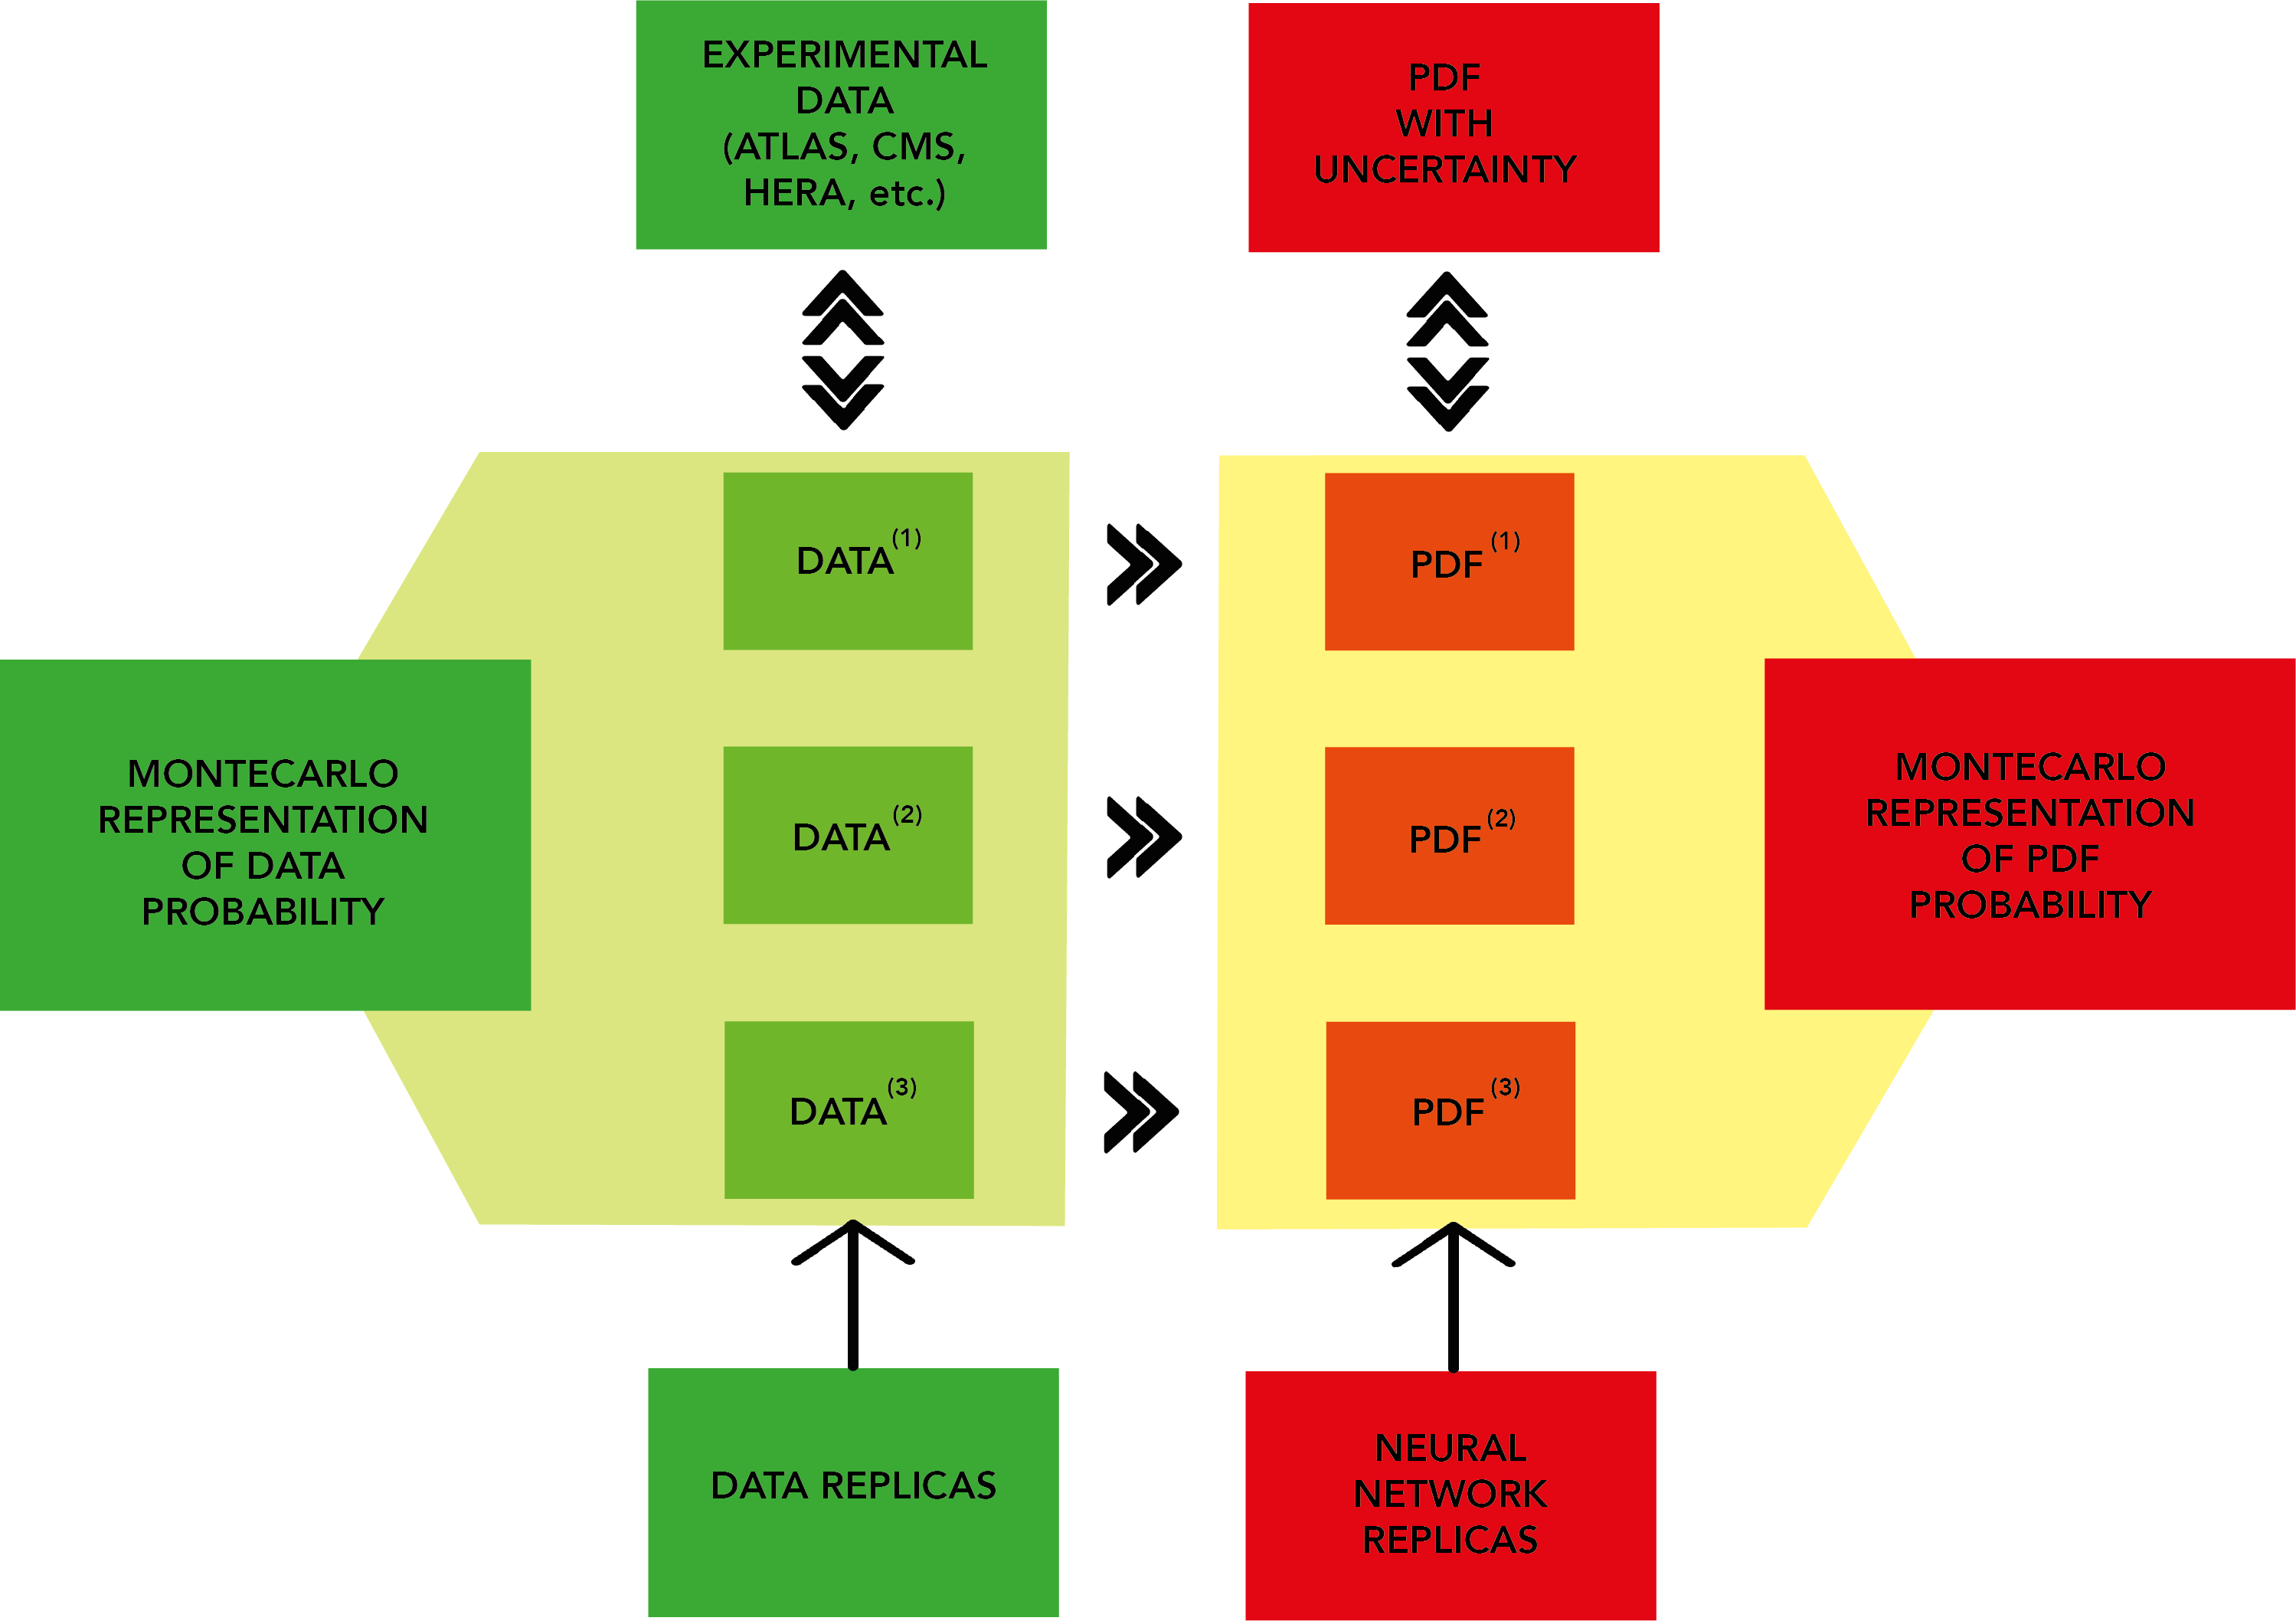
\includegraphics[width=0.8\textwidth]{background/generalstrategy.png}
\caption{NNPDF general strategy.}
\label{fig:generalstrategy}
\end{figure}
Once the pseudodata have been generated, each of these ($D^{(k)}$) is fitted separately to the theoretical predictions by minimising a target error function based on the $\chi^2$ (Eqn. \ref{eqn:chi2}), resulting in a PDF set of each flavour, $f_q^{(k)}$ (where $q$ runs over the fitted flavours: $g$, $u$, $d$, $s$, $c$, $\bar{u}$, $\bar{d}$, $\bar{s}$, $\bar{c}$). These act as a Monte Carlo parametrisation of the PDFs (for example, Fig. \ref{fig:replicas}).  This means that the PDFs and their errors can be extracted by taking the means and standard deviations over the ensemble. The final PDFs are made publicly available as downloadable files on the LHAPDF website \cite{lhapdf, Buckley:2014ana}. 

\begin{figure}
\centering
    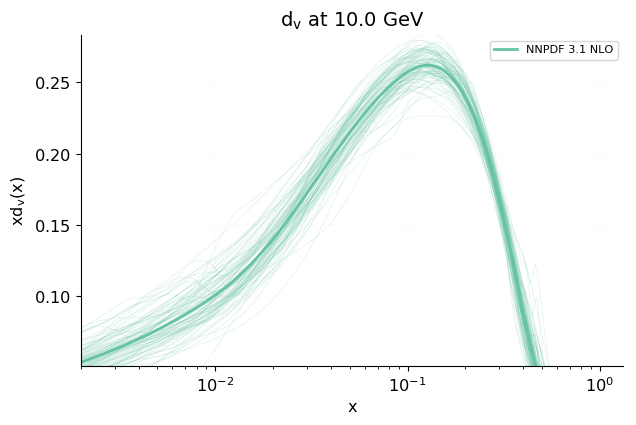
\includegraphics[width=0.7\textwidth]{background/Qs0_NNPDF31NLO_plot_pdfreplicas_d_v.png}
\caption{Monte Carlo replicas for the down valence quark PDF NNPDF3.1 at NLO. } \label{fig:replicas}
\end{figure}

\subsection{Neural Networks}

Inspired by how the brain processes information, in machine learning neural networks are a graph of connected nodes. They are trained by example, so
have the capability to learn a PDF's functional form given a set of data. The use of neural networks rather than specific functional forms allows us to avoid the theoretical bias which goes into selecting such a functional form. The layout, or ``architecture", consists
of input layers, hidden layers and output layers. Nodes can be either input nodes or activation nodes, the latter of which have an associated activation function which is applied to their output. Fig. \ref{fig:nn} depicts the architecture currently used by NNPDF. This is a ``2-5-3-1" archiecture, where the numbers refer to the number of nodes in each layer. It is a ``multilayer perceptron", meaning the graph is fully connected, and it is a feed-forward; information can only be passed in one direction through the layers (from 
input to output). The two inputs are $x$ and $\ln (1/x)$, and the output, $f$, is the PDF at the parametrisation scale, $Q_0$. In this network the output
of a node in the $l^{th}$ layer is given by
\beq
  \xi_i^{(l)} = g \bigg( \sum_j^{inputs} \omega_{ij}^{(l)} \xi_j^{(l-1)} + \theta_i^{(l)} \bigg)
\eeq
where the $\omega$s and $\theta$s are ``weights'' and ``thresholds''; parameters to be minimised
with respect to.  $g$ is an ``activation function'' which is set to
\beq
  g(z) =
\begin{cases}
 \frac{1}{1 + e^{-z}} &\text{for hidden layers}\\
  a &\text{for output layer}.
\end{cases}
\eeq
The choice of sigmoid activation function for the hidden layers allows sufficient non-linear freedom in the functional form, and the linear activation function for the output layer ensures the range of the PDFs is not restricted to [0,1].
\begin{figure}[H]
\centering
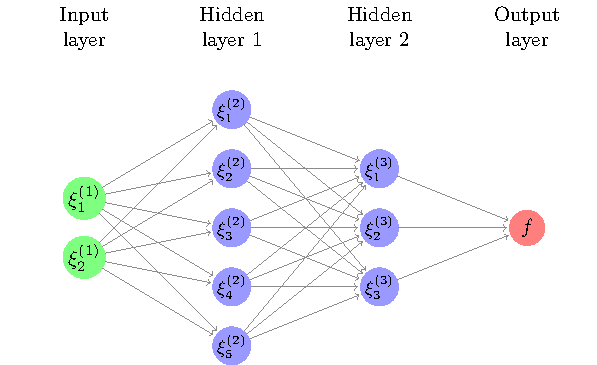
\includegraphics[width=\textwidth]{../diagrams/neuralnet.pdf}
\label{fig:nn}
\caption{Schematic depiction of the 2-5-3-1 architecture of an artificial neural network currently used by NNPDF. In the NNPDF methodology $\xi_1^{(1)}$ and $\xi_2^{(1)}$ are the variables $x$ and $\log x$ respectively.}
\end{figure}

The training of the neural networks is implemented using a ``genetic algorithm" (CMA-ES), so-called because of the introduction of mutation to the fitting parameters. This additional degree of randomness helps to avoid getting stuck in local minima. In practice, this involves ``mutating" some chosen fraction of the thresholds, $\theta$, by perturbing them at random.

\subsection{Parametrisation, preprocessing and postprocessing}
A scale of $Q=1.65$ $GeV$ is chosen to parametrise the PDFs at, and then they can be determined at any other scale by evolution using the DGLAP equations (Eqn. \ref{eqn:DGLAP}). The PDFs are fitted parametrised in a ``fitting basis", to help convergence \cite{Ball:2014uwa}, defined:
\begin{itemize}
\item $g$;
\item $\Sigma \equiv \sum_{u,d,s} q_i + \bar{q}_i$;
\item $T_3 \equiv u - d$;
\item $T_8 \equiv u + d - 2s$;
\item $V \equiv \sum_{u, d, s} q_i - \bar{q}_i$;
\item $V_3 \equiv \bar{u} - \bar{d}$;
\item $V_8 \equiv \bar{u} - \bar{d} - 2 \bar{s}$;
\item $c$.
\end{itemize}
Since the form of the neural networks ($N_i(x)$) is determined by training on experimental data, the output is not meaningful outwith the data region. The functional form of the PDFs in this so-called ``extrapolation region" is in practice fixed through enforcement of the known high and low $x$ behaviour via ``preprocessing"; the PDFs are parametrised as:
\beq
  f_i(x) = A_i x^{-\alpha_i} (1-x)^{\beta_i} N_i(x).
\eeq
$A_i$ are normalisation coefficients set by the sum rules and fixed at each iteration of the fit. The powers $\alpha_i$ and $\beta_i$ are fitted parameters determined by iteration from one fit to the next. This preprocessing has the effect that the PDFs approach 0 at large $x$, and generally grow at small $x$. This is because the probability of the existence of a parton is generally small at high $x$ and larger with decreasing $x$ outwith the data region.

Postprocessing is also applied to the PDF replicas to remove those which don't satisfy certain quality conditions. That is, where the target error function or arc-length of the replica is more than four standard deviations outwith the mean, or where the positivity of the resulting cross-sections is not satisfactorily maintained. 

\subsection{Cross validation}
Neural networks are effective at learning the functional form underlying data. Sometimes they can be ``too effective", picking up not just the underlying law but also the noise. This is known as ``overlearning" (see Fig. \ref{fig:overlearning} for an example).

\begin{figure}[H]
\centering
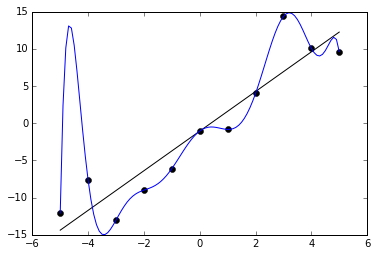
\includegraphics[width=0.6\textwidth]{background/overfitteddata.png}
\label{fig:overlearning}
\caption{Overlearning: the data points (black dots) fluctuate around the linear underlying law (black line), but the neural network continues to minimise the error function until it passes through every data point (blue curve), fitting the noise in the data.}
\end{figure}

To circumvent this problem, the data is split into a training and a validation set. The training data is used to optimise the neural network, and the validation data is used to test the network output, in a process known as ``cross validation". As training epochs elapse, the target error function compared to both the training and validation data should decrease as the network learns the underlying law. At some point, however, the network will begin to learn the noise in the training data, at which point the training error function will continue to decrease, but the validation error function will stop decreasing and start to increase again. The optimum fit is determined using the ``lookback" method, where after training the model corresponding to the minimum in the validation error function is selected.

\begin{figure}[H]
\centering
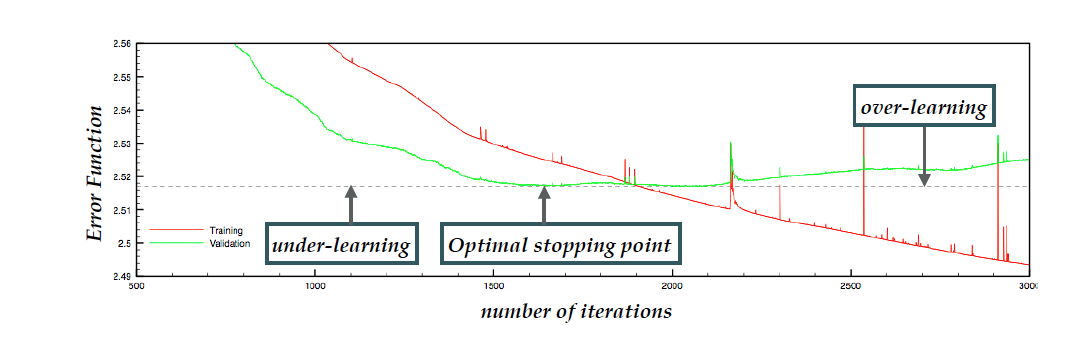
\includegraphics[width=\textwidth]{background/crossvalidation.png}
\label{fig:crossvalidation}
\caption{Cross validation with the lookback method.}
\end{figure}

\begin{figure}[H]
\centering
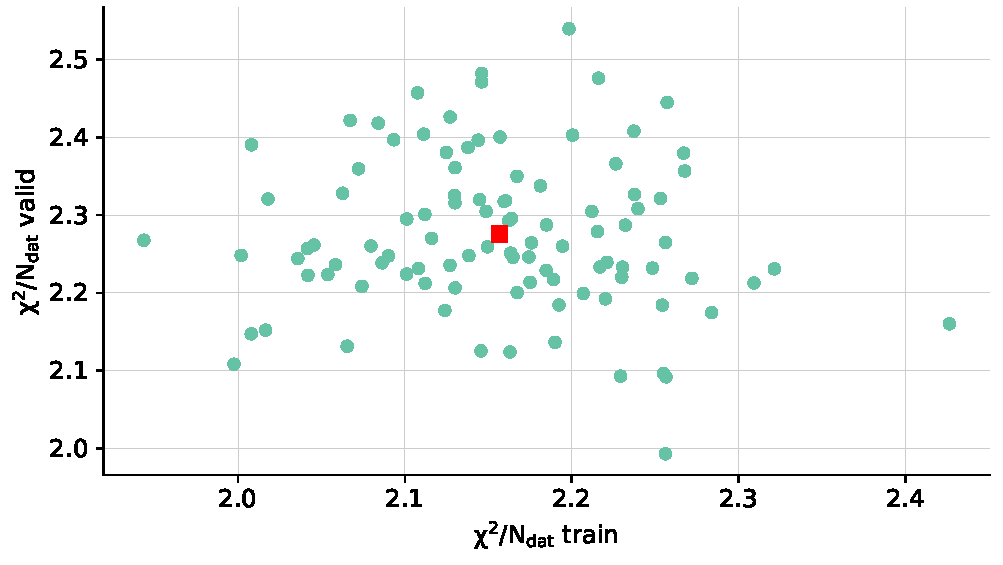
\includegraphics[width=\textwidth]{background/trvalchi2.pdf}
\label{fig:crossvalidation}
\caption{Comparing the training and validation $\chi^2$s for the 100 replicas (green circles) of a PDF fit. The red square gives the average.}
\end{figure}

\chapter{Theory uncertainties in PDFs - 10\%}
\bi 
\item What are theory uncertainties?
\item Why are they now important?
\item Types of unc - see below
\item Bayesian interpretation of these uncertainties - there is one "true" value e.g. for the higher order value, so need to estimate uncertainty bc will never know the size of e.g. MHOU unless you go ahead and calc - maybe ref d'Agostini paper on Bayesian interpretation
\item Will use Bayesian framework and assume Gaussianity of the expected true value of theory calc
\item Show C+S in fit - plus sign because exp and th unc are independent so combine errors in quadrature. They are also on an equal footing in terms of their effect on the PDFs
\item When many datasets/global fit, can have v strong theory correlations even across different experiments, because the underlying theory connects them

\ei
\section{Fitting PDFs including theory uncertainties}
Historically, experimental uncertainties have been the dominant source of error in PDF fits. 
In the NNPDF framework both replica generation and computation of $\chi^2$ 
are currently based entirely on these. We must now try to match the ongoing drive to 
increase experimental precision by including errors introduced at the theoretical level. This is
especially important given recent data sets such as the $Z$ boson transverse momentum
distributions~\cite{Aad:2014xaa,Khachatryan:2015oaa,Aad:2015auj}, which have very high experimental precision. Without
the inclusion of theoretical errors, this has led to tension with the other datasets.

In future NNPDF fits theoretical uncertainties will be included following a procedure outlined
by Ball \& Desphande \cite{Ball:2018odr}. This hinges on a result from Bayesian statistics
which applies to Gaussian errors. Namely, theory uncertainties can be included by directly 
adding a theoretical
covariance matrix to the experimental covariance matrix prior to the fitting. A brief summary of
the derivation is given below.

When determining PDFs we incorporate information from experiments in the form of $N_{dat}$ experimental data points $D_i$, $i=1,...,N_{dat}$. The associated uncertainties and their correlations are encapsulated in an experimental covariance matrix $C_{ij}$. Parts of the matrix which associate two independent experiments will be populated by zeros. However we would expect there to be correlations between data points from the same detector, for example.

Each data point is a measurement of some fundamental ``true" value, $\truev_i$, dictated by the underlying physics. In order to make use of the data in a Bayesian framework, we assume that the experimental values follow a Gaussian distribution about the unknown $\truev$. Then, assuming the same prior for $D$ and $\truev$, we can write an expression for the conditional probability of $\truev$ given the known data $D$:
\beq
\label{eqn:gaussexp}
P(\truev|D) = P(D|\truev) \propto \exp\bigg( -\frac{1}{2}(\truev_i-D_i)C_{ij}^{-1}(\truev_j - D_j)\bigg).
\eeq
However, in a PDF fit we cannot fit to the unknown true values $\truev$, and must make do with predictions based on current theory $T_i$. This is the origin of theory uncertainties in PDF fits; where our theory is incomplete, fails to describe the physics well enough, or where approximations are made, we will introduce all kinds of subtle biases into the PDF fit. The theory predictions themselves also depend on PDFs, so uncertainties already present in the PDFs are propagated through. This, in particular, leads to a high level of correlation because the PDFs are universal, and shared between all the theory predictions. 

We can take a similar approach when writing an expression for the conditional probability of the true values $\truev$ given the available theory predictions $T$, by assuming that the true values are Gaussianly distributed about the theory predictions.
\beq
\label{eqn:gausstheory}
P(\truev|T) = P(T|\truev) \propto \exp\bigg( -\frac{1}{2}(\truev_i-T_i)S_{ij}^{-1}(\truev_j - T_j)\bigg),
\eeq
where $S_{ij}$ is a ``theory covariance matrix" encapsulating the magnitude and correlation of the various theory errors. We will need to do some work to determine $S_{ij}$ for the different sources of error, and this will be outlined in detail in the following chapters. 

When we fit PDFs we aim to maximise the probability that a PDF-dependent theory is true given the experimental data available. This amounts to maximising $P(T|D)$, marginalised over the unknown true values $\truev$. To make this more useful for fitting purposes, we can relate this to $P(D|T)$ using Bayes' Theorem:
\beq
P(D|T)P(\truev |DT) = P(\truev |T)P(D|\truev T),
\eeq
where we note that the experimental data $D$ do not depend on our modelled values $T$, so $P(D|\truev T) = P(D|\truev)$. So we can integrate Bayes' Theorem over the possible values of the $N$-dimensional true values $\truev$:
\beq
\int D^N \truev P(D|T)P(\truev |DT) = \int D^N \truev P(\truev |T) P(D|\truev), 
\eeq
and, because $\int D^N \truev P(\truev |TD) = 1$ as all possible probabilities for the true values must sum to one, 
\beq
P(D|T) =  \int D^N \truev P(\truev |T) P(D|\truev). 
\eeq
We can always write the theory predictions $T$ in terms of their shifts $\D$ relative the true values $\truev$:
\beq
\D_i \equiv \truev_i - T_i.
\eeq
These shifts quantify the accuracy of the theoretical predictions, and can be thought of as nuisance parameters in the PDF fit. We can express the above integral in terms of the shifts $\D_i$, making use of the assumptions of Gaussianity in Eqns. \ref{eqn:gaussexp} and \ref{eqn:gausstheory}:
\beq
\begin{split}
\label{eq:probdatgivth}
P(D|T) &\propto \int D^N \D \exp \bigg(-\frac{1}{2}(D_i - T_i -\D_i)\\
&\times C_{ij}^{-1} (D_j -T_j -\D_j) - \frac{1}{2}\D_i S_{ij}^{-1} \D_j \bigg).
\end{split}
\eeq
To evalute the Gaussian integrals, consider the exponent: switching to a vector notation for the time being, we can expand this out and then complete the square, making use of the symmetry of $S$ and $C$:
\bdm
(D-T-\D)^T C^{-1}(D-T-\D) + \D^T S^{-1} \D  
= D^T(C^{-1} + S^{-1})\D -\D^T C^{-1} (D-T)
 - (D-T)^T C^{-1}\D + (D-T)^T C^{-1}(D-T) 
= (\D - (C^{-1} + S^{-1})^{-1} C^{-1}(D-T))^T(C^{-1}+S^{-1}) 
\times (\D - (C^{-1} + S^{-1})^{-1} C^{-1}(D-T)) 
-(D-T)^TC^{-1}(C^{-1} + S^{-1})^{-1}C^{-1}(D-T) 
+(D-T)^T C^{-1}(D-T).
\edm
Now, integrating Eqn. \ref{eq:probdatgivth} over $\D$ leads to a constant from the Gaussian integrals, which we can absorb, and only the parts of the exponent without $\D$ remain:
\bdm
P(T|D) = P(D|T) \propto \exp \bigg(-\frac{1}{2}(D-T)^T (C^{-1}-C^{-1}(C^{-1}+S^{-1})^{-1}C^{-1})(D-T) \bigg).
\edm
We can further simplify this by noting that
\bdm
(C^{-1}+S^{-1})^{-1} = (C^{-1}(C+S)S^{-1})^{-1} = S(C+S)^{-1}C,
\edm
which means we can rewrite
\bdm
C^{-1}-C^{-1}(C^{-1}+S^{-1})^{-1}C^{-1} = C^{-1} - C^{-1}S(C+S)^{-1} = (C^{-1}(C+S)-C^{-1}S)(C+S)^{-1} =(C+S)^{-1}.
\edm
Finally, with indices restored we are left with 
\bdm
P(T|D) \propto \exp \bigg(-\frac{1}{2}(D_i-T_i)(C+S)^{-1}_{ij}(D_j-T_j) \bigg).
\edm
Comparing this result to Eqn. \ref{eqn:gaussexp}, we can confirm that when we possess theoretical predictions, $T_i$, rather than true values, $\truev_i$, we can account for this by adding a theoretical covariance matrix, $S_{ij}$ to the experimental covariance matrix, $C_{ij}$ \cite{Ball:2018odr}. This means the theory uncertainties are on an equal footing with experimental systematic uncertainties. Note that $C_{ij}$ is positive definite by construction and so $(C+S)_{ij}$ is always invertible, even if $S_{ij}$ has negative eigenvalues.

Now all that remains is to construct a theory covariance matrix which parametrises each instance of theoretical uncertainty. This is a nebulous task, given that we are not privy to the true values, $\truev$, and so are unable to simply apply the formal definition
\beq
S_{ij} = \langle (\truev_i - T_i) (\truev_j - T_j) \rangle,
\eeq
where $\langle \cdot \rangle$ denotes an average over true values, $\truev$. We need to find methods to calculate the various contributions $S_{ij}$ (be them MHOUs, nuclear corrections, higher twist corrections etc.) which not only encapsulate the per-point theoretical errors but also preserve the correlations between different data points. Unlike experimental uncertainties, these correlations can exist outwith individual experiments; in fact, all data in PDF fits depend themselves on PDFs, and this common link will lead to correlations between all datapoints, albeit of varying strength. 

The following chapters address several important types of theoretical uncertainties: MHOUs; nuclear uncertainties; deuteron uncertainties. For each type, we show how to construct a theoretical covariance matrix, and present and discuss the results of PDF fits including these covariance matrices.

\chapter{Missing higher order uncertainties}

In this chapter we address the dominant source of theoretical uncertainty in current PDF fits: missing higher order uncertainties (MHOUs). In Sec.~\ref{sec:intro} we explain their origin, then in Sec.~\ref{sec:svn} we revise their standard method of estimation, through scale variation. We then show how to use this to construct a theory covariance matrix (Sec.~\ref{sec:prescrip}), and test the validity of this at NLO against the known NNLO result (Sec.~\ref{sec:valid}). Finally, we present the PDFs including MHOUs (Sec.~\ref{sec:pdfs}) and assess the impact on relevant phenomenology (Sec.~\ref{sec:mhoupheno}).

\section{Introduction}
\label{sec:intro}
PDF fits rely on the comparison of experimental data with theoretical predictions at the partonic level. These predictions are carried out in the framework of perturbation theory, where results are expressed as an expansion in the strong coupling constant, $\alpha_s$. The first non-zero contribution to the expansion is known as ``leading order" (LO), the next is ``next-to-leading order" (NLO), and so on (NNLO, N$^3$LO etc.). Because in the perturbative regime $\alpha_s$ is small (0.118 \cite{pdg}), corrections from higher orders are increasingly small. Predictions must be directly calculated at each order by considering all the possible contributing Feynman diagrams, and this becomes exponentially more complicated with increasing orders; the cutting edge of calculations is currently at the N$^3$LO level. PDFs are fitted using predictions truncated at a given order, with NNLO PDFs being the modern standard. 

These missing higher order terms in the expansion for theory predictions lead to missing higher order uncertainties (MHOUs), which are currently the dominant source of error in PDF fits. We can see that going from LO to NLO to NNLO in Fig.~\ref{fig:pdf_order_comp} that the functional form of the PDF changes, and that the change from LO to NLO is greater than that from NLO to NNLO. MHOUs are currently not included in the PDF errors, justified historically by the claim that they are small compared to experimental contributions to the PDF error, especially at NNLO. This justification, however, is now on shakier ground with PDF uncertainties dropping as low as 1\% at the electroweak scale. QCD MHOU errors themselves are typically $\mathcal{O}$(1\%)~\cite{Campbell:2017hsr} and, with the current push to N$^3$LO precision, will only become increasingly important as time goes on. 

\begin{figure}[!t]
\centering
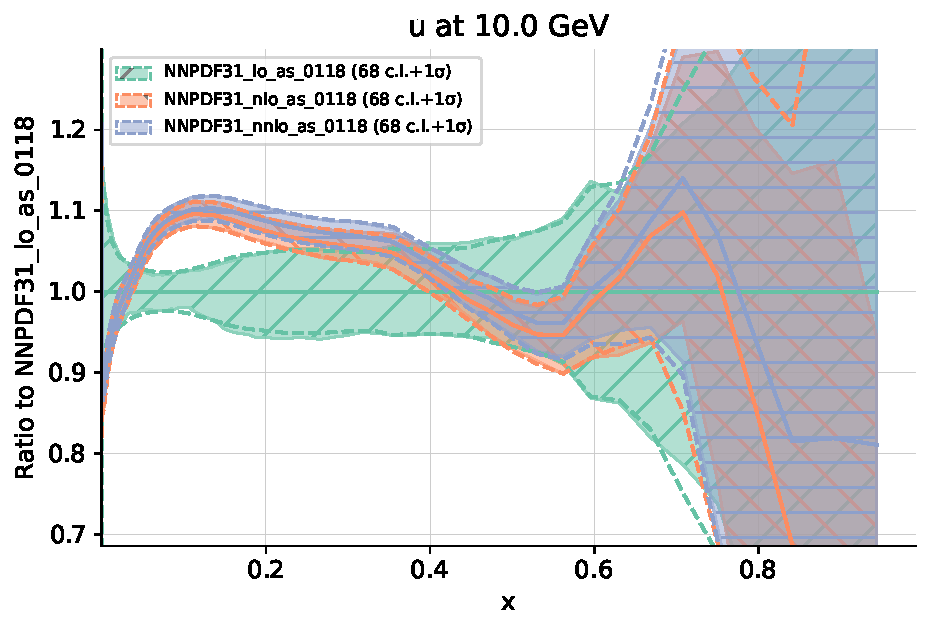
\includegraphics[width=0.49\linewidth]{mhous/plots/pdfscalespecs1_basespecs0_pdfnormalize1_plot_pdfs_u.pdf}
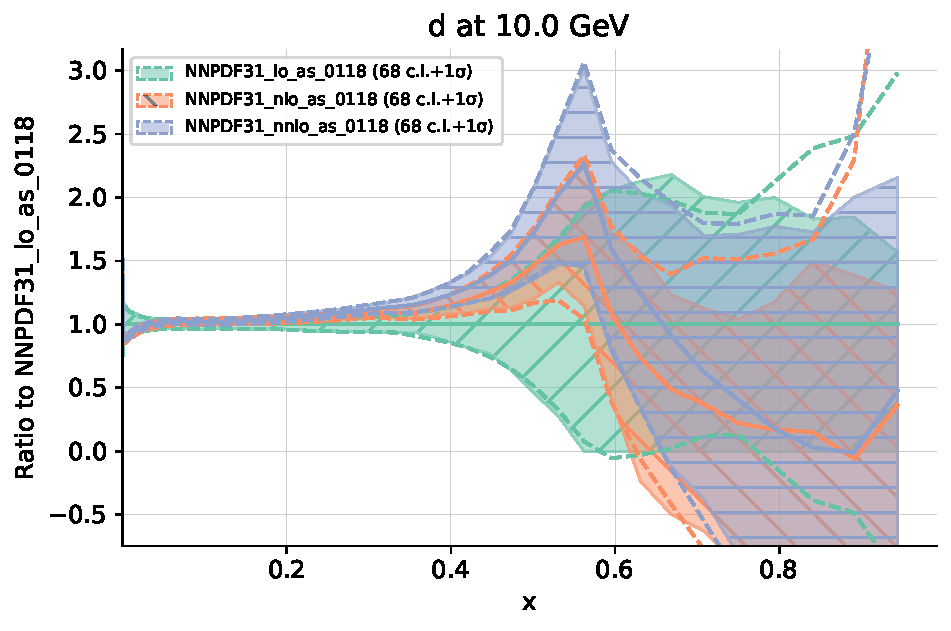
\includegraphics[width=0.49\linewidth]{mhous/plots/pdfscalespecs1_basespecs0_pdfnormalize1_plot_pdfs_d.pdf}\\
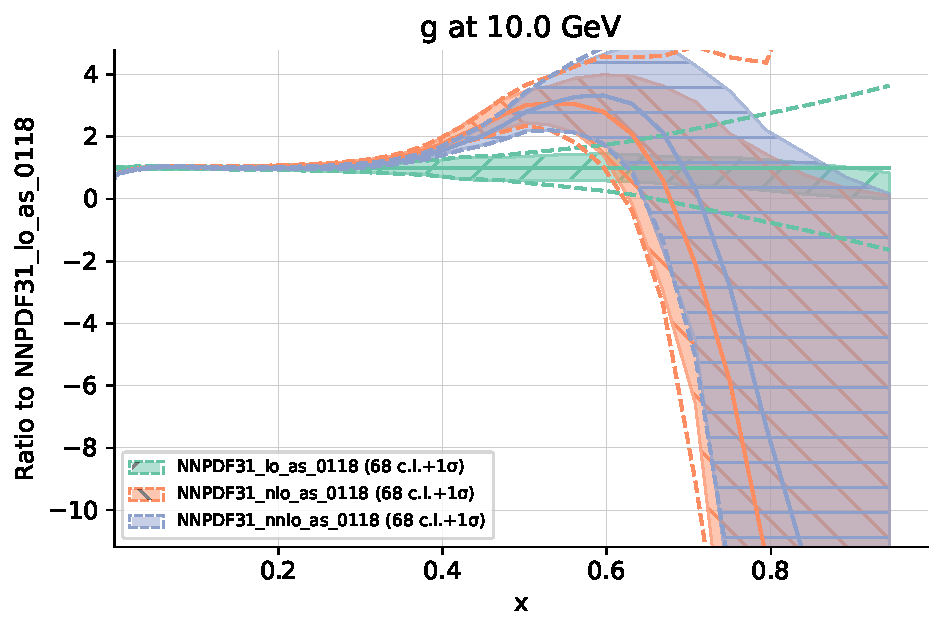
\includegraphics[width=0.49\linewidth]{mhous/plots/pdfscalespecs1_basespecs0_pdfnormalize1_plot_pdfs_g.pdf}
\caption{Comparison of NNPDF3.1 PDFs at different perturbative orders: LO (green); NLO (orange); NNLO (blue). PDFs are normalised to the LO result, and displayed at scale $Q$ = 10 GeV.}
\label{fig:pdf_order_comp}
\end{figure}

In addition to a missing source of per-point uncertainty on each data point, MHOUs can affect a PDF fit more insidiously by impacting on the desired weight of data sets relative to one another; regions of data with high MHOU are naturally to be trusted less when used to determine the PDFs, and so should carry less weight in the fitting process. If MHOUs are included, these data will be deweighted automatically because they will carry higher uncertainty, however in the absence of MHOUs they may impact on a fit to an undesirable degree.

Having established the importance of including MHOUs, in the next section we will go on to develop a formalism for estimating them, and constructing a MHOU covariance matrix.

\section{Scale variation}
\label{sec:svn}

The most popular method for estimating MHOUs is by ``scale variation". This is based on making theoretical predictions at a range of values of the artificial renormalisation ($\mu_R$) and factorisation ($\mu_F$) scales introduced in Chapter~\ref{chapter:background}. The renormalisation group equation (RGE;~\ref{eqn:rge}) and factorisation theorem only hold to all orders in perturbation theory, and in this case varying the scale values will have no effect on any results. However, when the perturbative expansion is truncated, there will be a residual $\mu_R$ and $\mu_F$ dependence which characterises the degree of MHOU. Varying these scales and observing the impact on the predictions can therefore provide an estimate of the MHOUs. 

Although other approaches to estimating MHOUs, based on the current known orders, have been suggested~\cite{Cacciari:2011ze, David:2013gaa, Bagnaschi:2014wea}, we adopted the method of scale variations not only because it is the most widely used, but also because it is the most easily implemented for our purposes. Firstly, the renormalisation group invariance is incorporated automatically, which ensures the MHOUs decrease as the perturbative order increases. Secondly, the scale dependece of $\alpha_s(\mu_R^2)$ and the PDFs is universal to all processes, which is important for PDF fits dealing with a range of interactions. Finally, correlations between data points are implicitly maintained because predictions for different scale values will be smooth functions of kinematics; this ensures that neighbouring regions of phase space will be strongly correlated.

There are, however, some disadvantages. Firstly, the definition of the two scales themselves have been historically approached in various ways, often differently for DIS and hadronic collisions, but also changing over time. Since PDFs use both DIS and hadronic data we need to settle on a consistent approach. Secondly, there is no cut and dry method for determining the range of varied scale choices, and in fact the choice of central scales are themselves to some degree arbitrary; for example, top production processes commonly have both central scales set to the top mass, $m_t$, and DIS processes have both set to Bj\"orken $Q$. Though there is physical motivation for these choices, we could equally well pick 2$m_t$ rather than $m_t$ in the former case, for example. A standard approach is to take the 7-point envelope of the predictions obtained by varying $(\mu_F, \mu_R)$ independently in $\{1/2, 1, 2\}$, excluding $(1/2, 1/2)$ and $(2,2)$. However, for our purposes we do not want a per-point envelope but rather a covariance matrix which retains correlations between data points. We will address both of these drawbacks below. 

Finally, scale variation techniques will not pick up any ``new physics" at higher orders, be it additional colour configurations, singularities or mechanisms of interaction. This is harder to deal with, and requires resummation techniques among other methods. In this work we assume these effects to be less important, and do not address them for the time being.

In the remainder of this section we will review the technique of scale variation, and with it the definitions of $\mu_F$ and $\mu_R$. We will converge on a genral formalism that can be applied to both electroproduction and hadroproduction. We will show that there are two independent directions of scale variation and discuss how to combine them, both in single process and multi-process interactions. We will then go on to show how to use this to build a covariance matrix in Sec.~\ref{sec:prescrip}.

\subsection{Renormalisation group invariance}

It is customary when making a theory prediction to pick a renormalisation scale, $\mu_R$, that is indicative of the physical scale of the interaction, $Q$. We will denote this ``central" theory prediction by $T(Q^2)$. In general, a theory prediction at scale $\mu_R$ can be written
$\overline{T}(\alpha_s(\mu_R^2), \mu_R^2/Q^2)$, where we explicitly note that $\alpha_s$ itself depends on the renormalisation scale. From this we can see that
\beq
T(Q^2) \equiv \overline{T}\big(\alpha_s(Q^2), 1 \big).
\eeq
The strong coupling constant satisfies the RGE
\beq \label{eqn:beta}
\mu_R^2 \frac{d^2}{d\mu_R^2}\alpha_s(\mu_R^2) = \beta \big( \alpha_s (\mu_R^2) \big),
\eeq
and we can expand the beta function perturbatively as
\beq 
\beta(\alpha_s) = \beta_0 \alpha_s^2 + \beta_1 \alpha_s^3 
+ \beta_2 \alpha_s^4 + \ldots \, .
\eeq

As discussed in Chapter~\ref{chapter:background}, renormalisation group invariance tells us that a prediction of a physical quantity (such as $\overline{T}$) to all orders must be independent of $\mu_R$, because this scale is unphysical. This means we can write
\beq \label{eqn:rgetbar}
  \mu_R^2 \frac{d}{d \mu_R^2} \overline{T} \lp
  \alpha_s(\mu_R^2), \mu_R^2/Q^2\rp  = 0 .
\eeq

Before proceeding further, we introduce some variables to make the analysis clearer:
\beq \label{eqn:notn}
\mu_R^2 = k Q^2,\qquad t = \ln (Q^2 / \Lambda^2), \qquad \kappa = \ln k = \ln \mu_R^2/Q^2,
\eeq
where $\Lambda$ is the QCD scale. This means $\alpha_s(\mu_R^2)$ is a function of $\ln \mu_R^2/\Lambda^2 = t + \kappa$.

Revisiting Eqn.~\ref{eqn:rgetbar}, we can write this as
\bea \label{eqn:newrge}
	0 & =& \frac{d}{d \kappa} \overline{T}(\alpha_s(t + \kappa), \kappa) \nonumber\\
	& =& \frac{d} {d \kappa} \alpha_s(t + \kappa) \frac{\partial}{\partial \alpha_s} \overline{T}(\alpha_s(t + \kappa), \kappa) \bigg|_\kappa + \frac{\partial}{\partial \kappa} \overline{T}(\alpha_s(t + \kappa), \kappa) \bigg|_{\alpha_s}\nonumber, \\
\eea
assuming that $\overline{T}$ is analytic in $\alpha_s$ and $\kappa$. To simplify this we can use
\beq 
	\frac{d}{d \kappa} \alpha_s(t + \kappa) = \frac{d}{dt} \alpha_s(t + \kappa) = \frac{d}{d \ln \mu_R^2} \alpha_s(t + \kappa) = \beta(\alpha_s(t + \kappa) ) \, ,
\eeq
where we have used the definition of the beta function (Eqn.~\ref{eqn:beta}), and this means that
\beq
	0 = \frac{\partial}{\partial t} \overline{T}(\alpha_s(t + \kappa), \kappa) \bigg|_\kappa + \frac{\partial}{\partial \kappa} \overline{T}(\alpha_s(t + \kappa), \kappa) \bigg|_{\alpha_s} \, .
\eeq
We can now Taylor expand $\overline{T}(\alpha_s, \kappa)$ about the central scale $\mu_R^2 = Q^2 \implies k=1 \implies \kappa = 0$ for fixed $\alpha_s$: 
\bea
  \overline{T}(\alpha_s(t + \kappa), \kappa) &=& \overline{T}(\alpha_s(t + \kappa), 0)\nonumber\\&&\qquad\qquad +\kappa \frac{\partial}{\partial \kappa} \overline{T}(\alpha_s(t + \kappa), 0) \bigg|_{\alpha_s} + \half \kappa^2 \frac{\partial^2}{\partial \kappa^2} \overline{T}(\alpha_s(t + \kappa, 0)\bigg|_{\alpha_s} + \ldots \qquad \nonumber \\.
\eea
Then, using Eqn.~\ref{eqn:newrge}, we can replace $\frac{\partial}{\partial \kappa}$ with
$-\frac{\partial}{\partial t}$, and write
\bea \label{eqn:trelation}
\overline{T}(\alpha_s(t + \kappa), \kappa) &=& \overline{T}(\alpha_s(t + \kappa), 0) - \kappa \frac{\partial}{\partial t} \overline{T}(\alpha_s(t + \kappa), 0) \bigg|_\kappa \nonumber\\ &+& \half \kappa^2  \frac{\partial^2}{\partial t^2} \overline{T}(\alpha_s(t + \kappa), 0)\bigg|_\kappa + \ldots \nonumber\\
&=& T(t + \kappa) - \kappa \frac{d}{dt} T(t + \kappa) + \half \kappa^2  \frac{d^2}{dt^2} T(t + \kappa)+\ldots\>.
\eea
This tells us how to find a scale varied theoretical prediction, $\overline{T}$, in terms of the $t$ dependence of the central prediction, $T$. Furthermore, we can express this $t$ dependence as an $\alpha_s$ dependence using
\beq
\frac{d}{dt} T(t) = \frac{d \alpha_s(t)}{dt} \frac{\partial}{\partial \alpha_s} \overline{T}(\alpha_s(t), 0) = \beta(\alpha_s(t)) \frac{\partial}{\partial \alpha_s} \overline{T}(\alpha_s(t), 0).
\eeq
Noting that $\beta(\alpha_s) = \mathcal{O}(\as^2)$, we see that 
$\frac{1}{T} \frac{dT}{dt}
= \mathcal{O}(\alpha_s)$ and $\frac{1}{T} \frac{d^2T}{dt^2} =
\mathcal{O}(\alpha_s^2)$ etc. The pattern follows that every time a derivative is taken with respect to $t$ you pick up a power of $\alpha_s$ as a consequence of the chain rule in differentiating. Looking back at Eqn. \ref{eqn:trelation} it is clear that each power of $\kappa$ is associated with a power of $\alpha_s$. Expressing the theory prediction perturbatively as
\be
T = \alpha_sT_{\text{LO}} + \alpha_s^2 T_{\text{NLO}} + \alpha_s^3 T_{\text{NNLO}} + \ldots\> ,
\ee
we can match powers of $\alpha_s$ in Eqn. \ref{eqn:trelation} to obtain the expressions
\begin{align} \label{eqn:theoryshifts}
\begin{split}
	\overline{T}_{\text{LO}}(\alpha_s(t + \kappa), \kappa) & = T_{\text{LO}}(t + \kappa), \\
	\overline{T}_{\text{NLO}}(\alpha_s(t + \kappa), \kappa) & = T_{\text{NLO}}(t + \kappa) - \kappa\smallfrac{d}{dt}{T}_{\text{LO}}(t + \kappa), \\
	\overline{T}_{\text{NNLO}}(\alpha_s(t + \kappa), \kappa) & = T_{\text{NNLO}}(t + \kappa) - \kappa\smallfrac{d}{dt}{T}_{\text{NLO}}(t + \kappa) \\
	&+ \half\kappa^2  \smallfrac{d^2}{dt^2}{T}_{\text{LO}}(t + \kappa).
\end{split}
\end{align}

The difference between the scale varied prediction and the central scale prediction,
\be
\Delta(t,\kappa) = \overline{T}(\alpha_s(t + \kappa), \kappa) - T(t) \, .
\ee
can be used to estimate the MHOU. From Eqn.~\ref{eqn:theoryshifts} we find the explicit expressions for the theory uncertainties
\be 
\begin{split}
\Delta_{\text{LO}}(t,\kappa) & = T_{\text{LO}}(t + \kappa)-T_{\text{LO}}(t), \\
{\Delta}_{\text{NLO}}(t,\kappa) & = (T_{\text{NLO}}(t + \kappa) - \kappa\smallfrac{d}{dt}{T}_{\text{LO}}(t + \kappa))-T_{\text{NLO}}(t), \\
{\Delta}_{\text{NNLO}}(t, \kappa) & = (T_{\text{NNLO}}(t + \kappa) - \kappa\smallfrac{d}{dt}{T}_{\text{NLO}}(t + \kappa) \\
&+ \half\kappa^2  \smallfrac{d^2}{dt^2}{T}_{\text{LO}}(t + \kappa))-T_{\text{NNLO}}(t) \, .
\end{split}
\ee
At LO we can see that the uncertainty results entirely from the choice of $\kappa$, in other words of $\mu_R$ in the $\alpha_s$ evaluation. At NLO we can see that the leading part of $T_{\text{NLO}}(t + \kappa)$ is subtracted off by the $\mathcal{O}(\kappa)$ term, meaning that the uncertainty is reduced with respect to LO. At NNLO, in addition, the $\mathcal{O}(\kappa^2)$ term subtracts off the subleading dependence of $T_{\text{NNLO}}(t + \kappa) - \kappa\smallfrac{d}{dt}{T}_{\text{NLO}}(t + \kappa)$, and so the uncertainty is yet smaller. This pattern of decreased scale variation uncertainties with increased perturbative order reflects our general understanding of the behaviour of MHOUs.

It is also apparent that the size of MHOU depends on the value of $\kappa$, in other words on the size of scale variation. This introduces a degree of arbitrariness into MHOU estimation, with the historical empirical range of choice being $\kappa \in [-\ln 4, \ln 4]$. In practice, we must investigate the dependence of $\Delta$ on $\kappa$, using validation at lower orders against known higher orders to converge on a suitable prescription.  This will be addressed in Sec.~\ref{sec:prescrip}. 

We will now go on to show how RG invariance can be applied to processes involving hadrons, where the partonic cross section is also convolved with a PDF. We will show that in this scenario there are two independent scales, and thus two independent sources of MHOU: one from the $\alpha_s$ dependence in the hard cross section; the other from the anomalous dimensions in the PDF evolution.

\subsection{Scale variation in partonic cross sections}
\label{subsec:svpartonic}
We will start with DIS, where there is only one hadron then move to the case of hadron-hadron collisions, such as those carried out at the LHC. In each case we will consider RG invariance to find an expression for $\mu_R$ variation in the partonic observable, for the case where the PDF is evaluated at the physical scale. Scale variation in PDF evolution, i.e. the $\mu_F$ variation, will be addressed in the next section.
\subsubsection{Deep Inelastic Scattering}
For DIS processes, theory predictions are of the structure functions discussed in Chapter~\ref{chapter:background}. These can be expressed as a convolution of a parton level coefficient, $C$, with a PDF, $f$:
\be 
\label{eqn:strfn}
F(Q^2) = C(x, \alpha_s(Q^2)) \otimes f(x, Q^2),
\ee
where $\otimes$ is a convolution in the momentum fraction, $x$, and there is an implicit sum over parton flavours. There will be a MHOU in $F$ due to truncating the coefficient function, $C$, to fixed perturbative order.  We can estimate this by keeping the PDF scale (or factorisation scale) fixed and varying the renormalisation scale in $C$. This will result in a scale-varied structure function,
\be
    \overline{F}(Q^2, \mu_R^2) = \overline{C}(\alpha_s(\mu_R^2), \mu_R^2/Q^2)\otimes f(Q^2)\, ,
\ee
where we have made the $x$-dependence implicit and the scale dependence explicit in the coefficient function. We can use the quantities defined in Eqn.~\ref{eqn:notn} to write this as
\be 
    \overline{F}(t, \kappa) = \overline{C}(\alpha_s(t + \kappa), \kappa)\otimes f(t).
\ee
We know that the structure function, an observable, is RG invariant, and, because we are keeping the factorisation scheme fixed, the PDF is independent of $\mu_R$. This means that the coefficient functions must also obey RG invariance, and so in a parallel with Eqn.~\ref{eqn:trelation} we can write
\be	
\overline{C}(\alpha_s(t + \kappa), \kappa) = C(t + \kappa) - \kappa \smallfrac{d}{dt} C(t + \kappa) + \half \kappa^2  \smallfrac{d^2}{dt^2} C(t + \kappa)+\ldots,
\ee
where, like before, we denote the central scale quantities without a bar. In order to evaluate the derivatives, note that the coefficient function can be expressed as a perturbative expansion in $\alpha_s$,
\be 
C(t) = c_0 + \alpha_s(t) c_1 + \alpha_s^2(t) c_2 + \alpha_s^3(t) c_3 +\ldots, 
\ee
and that $\smallfrac{d}{dt}\alpha_s(t,\kappa) = \beta(\alpha_s(t, \kappa)$, where the beta function also admits the expansion in Eqn.~\ref{eqn:beta}. Explicitly, this leads us to
\be 
\begin{split}
\smallfrac{d}{dt}{C}(t) & = \alpha_s^2(t) \beta_0 c_1+ \alpha_s^3(t) (\beta_1c_1+2\beta_0c_2) + \ldots,\\
\smallfrac{d^2}{dt^2}{C}(t) & = 2\alpha_s^3(t) \beta_0^2 c_1+ \ldots,
\end{split}
\ee 
resulting in the perturbative expression for $\mu_R$ variation of $C$:
\be 
\begin{split}
\overline{C}(\alpha_s(t + \kappa), \kappa) = c_0 &+ \alpha_s(t + \kappa) c_1 + \alpha_s^2(t + \kappa) (c_2 - \kappa \beta_0 c_1)\\ 
&+\alpha_s^3(t + \kappa)\big(c_3-\kappa (\beta_1c_1+2\beta_0c_2)+ \kappa^2 \beta_0^2 c_1\big) + \ldots \, .
\end{split}
\ee 
Using Eqn.~\ref{eqn:strfn} we finally get an expression for the $\mu_R$ variation of $F$:
\be 
\begin{split}
\overline{F}(t, \kappa) = c_0\otimes f(t) &+ \alpha_s(t + \kappa) c_1\otimes f(t) + \alpha_s^2(t + \kappa)  \lp c_2 - \kappa \beta_0 c_1 \rp \otimes f(t)\\ 
&+\alpha_s^3(t + \kappa) \lp c_3-\kappa (\beta_1c_1+2\beta_0c_2)+ \kappa^2 \beta_0^2 c_1 \rp \otimes f(t) + \ldots\>. 
\end{split}
\ee.
In practice, when predicting scale varied observables, using these equations is relatively straightforward. Because the coefficients, $c_i$ and $\beta_i$, are already known to some order, the workflow consists of some basic algebra to create the new, scale varied, coefficients at each order from the central-scale coefficients at the surrounding orders.

\subsubsection{Hadron-hadron collisions}
Hadron-hadron collisions can be considered in a similar way to DIS, the difference being that the observable cross section, $\Sigma$, depends on two PDFs, one for each of the hadrons:
\be 
    \Sigma(t) = H(t)\otimes( {f}(t)\otimes  {f}(t)) \, ,
\ee
where $H$ is the parton level cross section and this time we have used $t = \ln (Q^2 / \Lambda^2)$ from the outset. Once again, there is an implicit sum over parton flavours. As before, we can vary $\kappa = \ln (\mu^2/Q^2)$ in $H$ whilst keeping $f$ fixed, so that
\be \label{eqn:svarhadronic}
  \overline{\Sigma}(t,\kappa) = \overline{H} (\as(t+\kappa), \kappa)\otimes(f(t)\otimes f(t)),
\ee 
where
\be 
\overline{H}(\alpha_s(t), \kappa) = H(t) - \kappa \smallfrac{d}{dt} H(t) + \half \kappa^2  \smallfrac{d^2}{dt^2} H(t)+\ldots\>. 
\ee
Because hadron-hadron collisions involve a range of processes, we consider a generic process starting at $O(\alpha_s^n)$ for $n \in \mathbb{Z}$, so that
\be 
H(t) = \alpha_s^n(t)h_0 + \alpha_s^{n+1}(t)h_1 + \alpha_s^{n+2}(t)h_2+ \ldots\>.
\ee
Once again using $\smallfrac{d}{dt}\alpha_s(t,\kappa) = \beta(\alpha_s(t, \kappa)$ and Eqn.~\ref{eqn:beta} we arrive at
\begin{equation}
\begin{split}
\smallfrac{d}{dt}{H}(t) & = n\alpha_s^{n-1}(t)\beta(\alpha_s) h_0 + (n+1)\alpha_s^n(t)\beta(\alpha_s) h_1 + \ldots \\
&= \alpha_s^{n+1} n \beta_0 h_0 + \alpha_s^{n+2} (n \beta_1 h_0 + (n+1) \beta_0 h_1) + \ldots\\
\smallfrac{d^2}{dt^2}{H}(t) & = \alpha_s^{n+2} n(n+1) \beta_0^2 h_0 + \ldots.
\end{split}
\end{equation}
Overall, to evaluate $\overline{\Sigma}$ we can therefore use Eqn.~\ref{eqn:svarhadronic} along with 
\bea  \label{eqn:svarH}
    \overline{H}(\alpha_s, \kappa) &=& \alpha_s^n h_0 + \alpha_s^{n+1} (h_1 - \kappa n \beta_0 h_0) \nonumber\\ &+&\alpha_s^{n+2} (h_2 - \kappa(n \beta_1 h_0 + (n+1) \beta_0 h_1) \nonumber\\ &&\qquad+ \half \kappa^2 n(n+1) \beta_0^2 h_1) + \ldots .
\eea
Again, to evaluate the scale varied cross section, all that is needed is to modify the coefficients at each order using those at the central scale for the surrounding orders.
\subsection{Scale variation in evolution of PDFs}
We now turn to the effects of scale variation in the PDFs themselves. This is a crucial contribution to MHOUs because the PDFs are common to predictions for all processes, and therefore responsible for widespread correlations in uncertainty. MHOUs in the PDFs arise from the truncation of the perturbative expansion of the splitting functions (or, in Mellin space, the anomalous dimensions) in the DGLAP evolution equations (Eqn.~\ref{eqn:DGLAP}) discussed in Chapter~\ref{chapter:background}. The scale evolution of the PDFs can be encapsulated in Mellin space in the equation
\be \label{eqn:mellindglap}
	\mu_F^2 \frac{d}{d \mu_F^2} f(\mu_F^2) = \gamma(\alpha_s(\mu_F^2)) f(\mu_F^2)\, ,
\ee
where the parton flavour indices are left implicit and the anomalous dimension, $\gamma$, can be expressed as an expansion in $\alpha_s$ as
\be  \label{eqn:anomdimexp}
\gamma(t) =  \alpha_s(t) \gamma_0 + \alpha_s^2(t) \gamma_1^2  + \alpha_s^3(t) \gamma_2^3 + \cdots .
\ee
Note that we refer to a separate factorisation scale, $\mu_F$, distinct from the renormalisation scale, $\mu_R$, in the previous section. This is because each scale is associated with a separate RGE and they are therefore independent; to explore the full space of scale variations they need to be considered separately. 

To solve for the PDF, we can integrate Eqn.~\ref{eqn:mellindglap} to give
\be \label{eqn:pdfint}
	f(\mu_F^2) = \text{exp}\bigg(\int_{\mu_0}^{\mu_F^2} \frac{d \mu^{2}}{\mu^{2}} \gamma(\alpha_s(\mu^{2}))\bigg) f_0 \, ,
\ee
where $f_0$ is the PDF at the initial scale, $\mu_0$. Note that the LHS is independent of the choice of $\mu_0$. To consider the effect of scale variations on the PDF, we can proceed similarly to Sec.~\ref{subsec:svpartonic}, defining 
\beq \label{eqn:notn2}
\mu_F^2 = k Q^2,\qquad t = \ln (Q^2 / \Lambda^2), \qquad \kappa = \ln k = \ln \mu_F^2/Q^2,
\eeq
and finding the scale varied anomalous dimension
\be \label{eqn:svanomdim}
	\overline{\gamma}(\alpha_s(t), \kappa) = \gamma(t) - \kappa
        \smallfrac{d}{dt}{\gamma}(t) + \half \kappa^2
        \smallfrac{d^2}{dt^2}{\gamma}(t) + \cdots .
\ee
Once again we can use the beta function expansion (Eqn.~\ref{eqn:beta}) alongside Eqn.~\ref{eqn:anomdimexp} to give
\bea \label{eqn:anomdimresult}
    \overline{\gamma}(\alpha_s(t + \kappa), \kappa) &=& \alpha_s(t+\kappa) \gamma_0 + \alpha_s^2(t+\kappa) (\gamma_1 - \kappa \beta_0 \gamma_0) \nonumber\\ &+& \alpha_s^3(t+\kappa) (\gamma_2 - \kappa (\beta_1 \gamma_0 + 2 \beta_0 \gamma_1) + \kappa^2 \beta_0^2 \gamma_0) \nonumber\\ &+& \cdots \, ,
\eea
which has the same form as Eqn.~\ref{eqn:svarH} upon setting $n=1$. We can use this equation to estimate MHOUs in PDFs, which can be done by refitting the PDF at each scale choice using different anomalous dimensions. This method has been applied in previous analyses~\cite{Martin:1990fq, Virchaux:1991jc, Ridolfi:1999vr}, but the process of refitting the PDFs is computationally intensive and so we would like to avoid having to do this if possible. Instead, we can look directly at the PDF level and consider evaluating the PDFs themselves at different scales, as was done in Ref.~\cite{Altarelli:2008aj}.  

We can define the scale varied PDF as that obtained by varying the scale in the anomalous dimension,
\be
\overline{f}(\as(t + \kappa), \kappa) = \text{exp}\bigg(\int_{t_0}^t dt' \overline{\gamma}(\alpha_s(t' + \kappa), \kappa)\bigg) f_0 \, 
\ee
Shifting integration variable $t' \to t'- \kappa$ whilst redefining the initial scale, we can then apply Eqn.~\ref{eqn:svanomdim} and expand the exponential, {\it i.e.}
\bea
\overline{f}(\as(t + \kappa), \kappa) &=& \text{exp}\bigg(\int_{t_0}^{t+\kappa} dt' \overline{\gamma}(\alpha_s(t'), \kappa)\bigg) f_0 \nonumber\\
&=& \exp\lp \lc \int_{t_0}^{t + \kappa} dt' \gamma(t')\rc  - \kappa  \gamma(t + \kappa) + \half \kappa^2 \frac{d}{dt} {\gamma}(t + \kappa) + \ldots \rp \nonumber\\
&& \times \exp\lp \kappa  \gamma(t_0) - \half \kappa^2 \frac{d}{dt} {\gamma}(t_0) + \ldots \rp f_0 \\
&=& \lc 1 - \kappa \gamma(t + \kappa) + \half \kappa^2
    (\gamma^2(t + \kappa)+\frac{d}{dt}{\gamma}(t + \kappa)) + \ldots
    \rc \nonumber\\
&& \times \exp\lp \int_{t_0}^{t + \kappa} dt' \gamma(t')\rp \exp\lp \kappa  \gamma(t_0) - \half \kappa^2 \frac{d}{dt} {\gamma}(t_0) + \ldots \rp f_0 \nonumber \, .
\eea
We can absorb the factor resulting from variation of $t_0$ into the initial PDFs, $f_0$, so that $\exp\lp \kappa  \gamma(t_0) - \half \kappa^2 \frac{d}{dt} {\gamma}(t_0) + \ldots \rp f_0 \to f_0$. Then, noting also that $\exp\lp \int_{t_0}^{t + \kappa} dt' \gamma(t')\rp f_0 = f(t + \kappa)$, we end up with the result
\be \label{eqn:pdfvarresult}
\overline{f}(\as(t + \kappa), \kappa) = \lc 1 - \kappa \gamma(t + \kappa) + \half \kappa^2
    (\gamma^2(t + \kappa)+\frac{d}{dt}{\gamma}(t + \kappa)) + \ldots
    \rc f(t+ \kappa) \, .
\ee
This result, which comes from varying the scale at which the PDF is evaluated, is equivalent to the result which comes from varying the scale in the anomalous dimension, Eqn.~\ref{eqn:anomdimresult}. This is because there is only one RGE and therefore only one scale which the PDF depends on. Furthermore, note that Eqn.~\ref{eqn:pdfvarresult} shows us that the scale dependence can be factorised out of the PDF. This means we are free to instead factor it into the parton level coefficient function, which will always appear convolved with the PDF. This is useful when making a scale varied prediction when only a central PDF is available, and has been used in the past to make predictions for new LHC processes (e.g. Higgs production~\cite{deFlorian:2016spz}). However, in the case where we also want to consider $\mu_R$ variation in the coefficient function, the two scale variations will be mixed up, and this can lead to a complicated interplay, especially in the presence of heavy quark effects. In this work we adopt the method of scale variation for PDFs by using Eqn.~\ref{eqn:pdfvarresult}. 

\subsection{Varying two scales together}
We now consider the simultaneous variation of $\mu_R$ in the parton level observable and $\mu_F$ in the PDFs, in order to explore the full range of scale variation space. We will derive formulae for scale variation up to NNLO which are needed to construct a MHOU covariance matrix. 

For a DIS process we can write the double-scale-varied structure function as
\be \label{eqn:doublesv}
\overline{F}(Q^2, \mu_F^2, \mu_R^2) = \overline{C}(\alpha_s(\mu_R^2), \mu_R^2/Q^2) \otimes \overline{f}(\alpha_s(\mu_F^2), \mu_F^2/Q^2).
\ee
Similarly to before, we can define the variables
\beq \label{eqn:notn3}
\mu_{(F/R)}^2 = k_{(F/R)} Q^2,\qquad \kappa_{(F/R)} = \ln k_{(F/R)}, \qquad t_{(F/R)} = t + \kappa_{(F/R)}
\eeq
and use them to write the structure function as
\be
    \overline{F}(t, \kappa_F, \kappa_R) = \overline{C}(t_R, \kappa_R)
    \overline{f}(t_F, \kappa_F).
\ee
We then need to apply the equations for the scale varied PDFs and coefficient functions from the previous section, 
\be 
\begin{split}
    &\overline{f} (t_F, \kappa_F) = f(t_F) - \kappa_F
  \smallfrac{d}{dt}{f}(t_F) + \half \kappa_F^2
  \smallfrac{d^2}{dt^2}{f}(t_F) + ... \, , \\ 
    &\overline{C} (t_R, \kappa_R) = C(t_R) - \kappa_R
  \smallfrac{d}{dt}{C}(t_R) + \half \kappa_R^2
  \smallfrac{d^2}{dt^2}{C}(t_R) + ...   \, ,
\end{split}    
\ee
and use the fact that $\smallfrac{\partial}{\partial t} \sim \mathcal{O}(\alpha_s)$ to see that
\bea
    \overline{F}(t, \kappa_F, \kappa_R) 
    &=& C(t_R)f(t_F) - \lp \kappa_F C(t_R) \smallfrac{d}{dt}{f} (t_F)
    + \kappa_R \smallfrac{d}{dt}{C}(t_R) f(t_F) \rp  \nonumber\\
    &&\qquad + \half\Big(  \kappa_F^2
    C(t_R) \smallfrac{d^2}{dt^2} f(t_F)  
    + 2\kappa_R \kappa_F
    \smallfrac{d}{dt}{C}(t_R)\smallfrac{d}{dt}{f}(t_F) \nonumber\\
    &&\qquad \qquad +
    \kappa_R^2 \smallfrac{d^2}{dt^2}{C}(t_R)f(t_F)\Big) +
    \mathcal{O}(\alpha_s^3) \, . 
\eea
Taking a closer look, and comparing to Eqn.~\ref{eqn:doublesv}, we can write this in terms of partial derivatives of $F$:
\bea
    \overline{F}(t, \kappa_F, \kappa_R)  &=& F(t_F,t_R) - \bigg( \kappa_F\ \frac{\partial F}{\partial t_F}\bigg|_{t_R} + \kappa_R\ \frac{\partial F}{\partial t_R}\bigg|_{t_F} \bigg) \nonumber\\
    &&\qquad+ \half \bigg( \kappa_F^2 \frac{\partial^2 F}{\partial t_F^2}\bigg|_{t_R} +  2 \kappa_F \kappa_R \frac{\partial^2 F}{\partial t_F \partial t_R} \nonumber \\ &&\qquad +  \kappa_R^2 \frac{\partial^2 F}{\partial t_R^2}\bigg|_{t_F} \bigg)  + \cdots \, .    
\eea
Considering this expression, we can think of $\kappa_F\smallfrac{\partial}{\partial t_F}$ and $\kappa_R\smallfrac{\partial}{\partial t_R}$ as being the generators of the two types of scale variations.

For hadronic-hadron processes, the double-scale-varied cross section is instead
\be 
\overline{\Sigma}(t_F, t_R, \kappa_F, \kappa_R) = \overline{H}(\as(t_R), \kappa_R)\otimes  \lp \overline{f}(t_F, \kappa_F)\otimes\overline{f}(t_F, \kappa_F) \rp \, .
\ee
and we can apply exactly the same approach as above, leading to 
\bea
    \overline{\Sigma}(t, \kappa_F, \kappa_R)  &=& \Sigma(t_F,t_R) - \bigg( 2\kappa_F\ \frac{\partial \Sigma}{\partial t_F}\bigg|_{t_R} + \kappa_R\ \frac{\partial \Sigma}{\partial t_R}\bigg|_{t_F} \bigg) \nonumber\\
    &&\qquad+ \half \bigg( 2\kappa_F^2 \frac{\partial^2 \Sigma}{\partial t_F^2}\bigg|_{t_R} +  4 \kappa_F \kappa_R \frac{\partial^2 \Sigma}{\partial t_F \partial t_R} \nonumber \\ &&\qquad +  \kappa_R^2 \frac{\partial^2 \Sigma}{\partial t_R^2}\bigg|_{t_F} \bigg)  + \cdots \, ,    
\eea
where this time we pick up a factor of 2 with each $\kappa_F\smallfrac{\partial}{\partial t_F}$, due to the two PDFs.
\subsection{Scale variation for multiple processes}
We are now approaching a formalism which can be applied to carry out scale variations for the data included in PDF fits. But first we need to work out how to carry out simultaneous scale variations involving data from more than one process, for example DIS and Drell-Yan. 

For the case of two separate processes, the parton level cross sections will be totally independent, so there will be two separate RGEs and therefore two separate renormalisation scales, and hence renormalisation scale variation should be uncorrelated. However, all the processes share a common factorisation scale, and so the factorisation scale variation must be correlated. 

This correlation can be complex because the DGLAP equation is a matrix equation, and the anomalous dimension matrix has several independent eigenvalues (at NLO there are two singlet and one non-singlet, and more at higher orders). In order to fully preserve the correlations we ought to consider a separate factorisation scale for each of these components, and fully correlate this across all processes. In this current work, however, we attempt to reduce the complexity by retaining full correlation in the factorisation scale, only varying one scale. This approximation might be inaccurate when considering two processes with evolution dependent on different anomalous dimensions, in which case we would not be fully exploring the scale variation space. We draw attention to this limitation as an area of future study.

Sticking for the time being with correlated factorisation scale variation, for two processes we will have in general three scales: two renormalisation scales and one factorisation scale; $\mu_{R_1}$, $\mu_{R_2}$ and $\mu_F$. If we vary each scale independently by a factor of 2 about their central value we will have seven total scale choices to consider. Each time we add another process we will add another renormalisation scale, and in effect add another dimension to the scale variation. For $p$ independent processes, labelled $a = 1, \ldots, p$, there will be $p+1$ independent scale parameters and $3 + 2p$ total scale variations; one variation is the central scale, two variations up and down for the factorisation scale, and two variations up and down for each of the $p$ renormalisation scales.
\section{Building the theory covariance matrix}
\label{sec:prescrip}
We now have all the components we need to set about constructing a theory covariance matrix; we can carry out double scale variation for both DIS and hadron-hadron processes, and correlate scale variation between multiple processes. All that remains is to formulate a prescription for estimating MHOUs given scale variations.

In Chapter~\ref{chapter:thuncs} we formulated a method for including theory uncertainties in PDFs using a theory covariance matrix composed using a distribution of shifts between theory predictions at fixed order and the unknown all-order ``true" theory. We know that scale variation can be used to provide an estimate of these shifts, but as discussed previously the exact combination of scales is arbitrary. To address this problem, we present a series of prescriptions for constructing the theory covariance matrix, which we will later go on to test using results at known orders and in addition by studying the impact on the PDFs; we can then select the best prescription.

We consider a set of data involving $p$ different types of processes, each with data points $\{i_a\}$, $a = 1, \ldots, p$ and an associated renormalisation scale ratio $\kappa_{R_a} = \ln \mu_{R_a}^2/Q^2$. The theory covariance matrix can be constructed by taking an average over the outer products of the shifts in scale varied theory relative to the central theory. For the $a$-th process, these shifts are
\be 
  \Delta_{i_a} (\kappa_F, \kappa_{R_a} ) \equiv
  T_{i_a}(\kappa_F, \kappa_{R_a}) - T_{i_a}(0,0) \, .
\ee
For a given prescription, $m$, we then choose a set of points, $V_m$, in $p+1$-dimensional scale variation space, and construct the theory covariance matrix by summing over these points, normalised by a prescription-dependent factor $N_m$:
\be 
  S_{ij} = N_m \sum_{V_m} \Delta_{i_a} (\kappa_f, \kappa_{R_a}) \Delta_{i_b} (\kappa_f, \kappa_{R_b}) \, .
\ee
Note that $a$ and $b$ can label either the same or different processes. Importantly, since the covariance matrix is assembled as a sum of outer products it will necessarily be positive semi-definite. However, given that the dimension of the data is $\mathcal{O}(1000)$ and the dimension of $V_m$ will be in general considerably smaller, we expect $S$ to be singular in most instances. 

It now remains to develop a prescription, $m$. We must consider the full set of data, so there are two scenarios:
\begin{enumerate}
\item $i$ and $j$ belong to the same process;
\item $i$ and $j$ belong to different processes.
\end{enumerate}
Because $S$ is rank 2, we only need to consider a maximum of two different processes at any one time. Finally, we can choose how to correlate the scale variation; we can pick a ``symmetric prescription", in which the scales are varied independently, or an ``asymmetric prescription", where they are correlated. This second scenario amounts to setting $\mu_F = \mu_R$, which is like varying the scale in the physical cross section; because in a central prediction we typically set both scales to the physical scale of the process (e.g. $Q$ for DIS), we can call this varying the scale of the process. 

\subsection{Symmetric prescriptions}
In a symmetric prescription, the scales are varied in an uncorrelated way.
\subsubsection{One process}
For a single process ($p=1$), there are two scales, $\kappa_F$ and $\kappa_R$. Let us denote the number of independent scales as $s$, so here $s=2$. We can write the theory covariance matrix as
\be 
  S_{ij} = n_{m} \sum_{v_{m}} \Delta_{i} (\kappa_F, \kappa_R)\Delta_{j} (\kappa_F, \kappa_R)\, ,
\ee
where $v_m$ is the set of $m$ scale-varied points and $n_m$ is a normalisation factor, to be determined. Note that $v_m$ excludes any points for which $\Delta_i$ vanishes, since these will not contribute to $S$. In practice, this means the central point ($\kappa_F = \kappa_R = 0$) is not included. Overall there is one central point and $m$ variations, so we typically refer to a given prescription as an ``$(m+1)$-point prescription". We can find $n_m$ by summing over the number of independent scales, $s$, and averaging over the contributions from each scale, $m$. This means we can write
\be
n_m = s/m.
\ee
We will now outline three different prescriptions, depicted in Fig.~\ref{fig:symmetricPrescriptions}. In each case we denote the values of the scales $(\kappa_F; \kappa_R)$, varying each by the fixed values $\kappa = \{0, \pm \ln 4\}$, which we denote $\{0, \pm\}$ respectively. We also adopt the notation $\Delta_i^{+0}=\Delta_i(+\ln 4,0)$, $\Delta_i^{0-}=\Delta_i(0,-\ln4 )$, etc. for the shifts.
%%%%%%%%%%%%%%%%%%%%%%%%%%%%%%%%%%%%%%%%%%%%%%%%%%%%%%%%%%%%%%%%%%%%%%%%%%%%%%%
\begin{figure}
\centering
{\begin{tikzpicture}
\draw[->] (-1.5,0) -- (1.5,0);
\draw[->] (0,-1.5) -- (0,1.5);
\filldraw[black] (0,0) circle (2pt);
\filldraw[black] (-1,0) circle (2pt);
\filldraw[black] (0,-1) circle (2pt);
\filldraw[black] (1,0) circle (2pt);
\filldraw[black] (0,1) circle (2pt);
\node at (0.5,1.5) {$\kappa_R$};
\node at (1.9,0) {$\kappa_F$};
\end{tikzpicture}}\qquad
{\begin{tikzpicture}
\draw[->] (-1.5,0) -- (1.5,0);
\draw[->] (0,-1.5) -- (0,1.5);
\filldraw[black] (0,0) circle (2pt);
\filldraw[black] (-1,-1) circle (2pt);
\filldraw[black] (1,1) circle (2pt);
\filldraw[black] (1,-1) circle (2pt);
\filldraw[black] (-1,1) circle (2pt);
\node at (0.5,1.5) {$\kappa_R$};
\node at (1.9,0) {$\kappa_F$};
\end{tikzpicture}}\qquad
{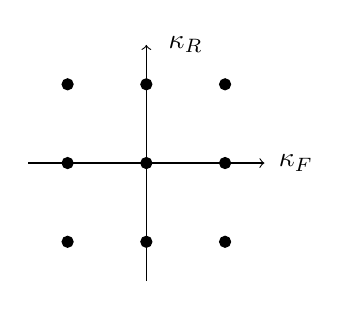
\begin{tikzpicture}
\draw[->] (-1.5,0) -- (1.5,0);
\draw[->] (0,-1.5) -- (0,1.5);
\filldraw[black] (0,0) circle (2pt);
\filldraw[black] (-1,0) circle (2pt);
\filldraw[black] (0,-1) circle (2pt);
\filldraw[black] (1,0) circle (2pt);
\filldraw[black] (0,1) circle (2pt);
\filldraw[black] (-1,-1) circle (2pt);
\filldraw[black] (1,-1) circle (2pt);
\filldraw[black] (-1,1) circle (2pt);
\filldraw[black] (1,1) circle (2pt);
\node at (0.5,1.5) {$\kappa_R$};
\node at (1.9,0) {$\kappa_F$};
\end{tikzpicture}}
\begin{caption}{Symmetric prescriptions for a single process, indicating
    the sampled values for the factorization scale $\kappa_F$ and 
    renormalization scale $\kappa_R$ in each case.
    %
    The origin of coordinates corresponds to the
    central scales $\kappa_f=\kappa_r= 0$.
    %
    We show the three prescriptions 
    $5$-point (left), $\bar{5}$-point (center) and $9$-point (right).
\label{fig:symmetricPrescriptions}
  }
\end{caption}
\end{figure}
%%%%%%%%%%%%%%%%%%%%%%%%%%%%%%%%%%%%%%%%%%%%%%%%%%%%%%%%%%%%%%%%%%%%%%%%%%%%%%%
\begin{itemize}
\item \textbf{5-point}: 
$v_4 = \{(\pm;0), (0; \pm) \}$ and $n_4 = 2/4 = 1/2$. This amounts to scale variation for each scale in turn, keeping the other fixed. We find the covariance matrix
\be \label{5S}
    S^{\rm (5pt)}_{ij} = \smallfrac{1}{2}\big\{ \Delta_i^{+0}\Delta_j^{+0} + \Delta_i^{-0} \Delta_j^{-0} + \Delta_i^{0+} \Delta_j^{0+} + \Delta_i^{0-} \Delta_j^{0-}  \big\} \, .
\ee
We find that the variations of each scale are added together in quadrature, as one would expect for independent contributions to the MHOU.
\item \textbf{$\overline{5}$-point}:
$\overline{v}_4 = \{(\pm; \pm) \}$, where $(\pm;\pm)$ are assumed
  uncorrelated, and $\overline{n}_4 = 2/4 = 1/2$. This is the complement of 5-point, exploring a different region of scale variation space.
\be
 \label{5bS}
    S^{(\rm \overline{5}pt)}_{ij} = \smallfrac{1}{2}\big\{ \Delta_i^{++}\Delta_j^{++} + \Delta_i^{--}\Delta_j^{--} + \Delta_i^{+-}\Delta_j^{+-} + \Delta_i^{-+} \Delta_j^{-+}\big\} \, .
\ee
\item \textbf{9-point}: $v_8=v_4\oplus \overline{v}_4$ (the union of 5-point and
  $\overline{5}$-point) and $n_8 = 2/8 = 1/4$. Here we include every combination, varying the scales totally independently. 
\be \label{9S}
\begin{split}
    S^{(\rm 9pt)}_{ij} = \smallfrac{1}{4}\big\{ &\Delta_i^{+0} \Delta_j^{+0} + \Delta_i^{-0}\Delta_j^{-0}
                            + \Delta_i^{0+} \Delta_j^{0+} + \Delta_i^{0-}\Delta_j^{0-} \\
                            + &\Delta_i^{++}\Delta_j^{++} + \Delta_i^{+-} \Delta_j^{+-}
                            + \Delta_i^{-+}\Delta_j^{-+} + \Delta_i^{--} \Delta_j^{--} \big\} \, .
\end{split}                            
\ee 
\end{itemize}
\subsubsection{Two processes}
\subsection{Asymmetric prescriptions}
\subsubsection{One process}
\subsubsection{Two processes}
\subsection{Categorising processes}
\subsection{NLO theory covariance matrices}

\section{Validating the theory covariance matrix}
\label{sec:valid}

\section{PDFs with missing higher order uncertainties}
\label{sec:pdfs}

\section{Impact on phenomenology}
\label{sec:mhoupheno}

\chapter{Nuclear Uncertainties}
\label{chapter:nuclear}
The theory covariance formalism developed in Chapter~\ref{chapter:thuncs} can be applied to any source of theory uncertainty in PDFs. One of the most important of these is nuclear uncertainties. A wide range of data is needed to pin down the form of PDFs, including that where the proton is not in a free state. More precisely, this encompasses DIS and DY fixed target measurements involving deuteron and heavy nuclear targets. In these cases the proton's interaction is altered due to the surrounding nuclear environment, and this difference propagates through to the fitted PDFs, leading to an unwanted shift in their central values and uncertainties. We cannot simply discard these data, as they play a crucial role in the strangeness content of the proton and also the light flavour separation at high $x$, a region important for searches for physics beyond the Standard Model. Instead, we must determine corrections to the PDF central value and additional uncertainties to account for the use of nuclear data.

Given their importance, there have been wide-ranging studies of deuteron and heavy nuclear corrections: deuteron corrections have been included in previous PDF determinations via nuclear smearing functions~\cite{Owens:2012bv,Ball:2013gsa,Harland-Lang:2014zoa,Accardi:2016qay,
  Alekhin:2017fpf} based on models of the deuteron wavefunction~\cite{Wiringa:1994wb,Melnitchouk:1994rv,Melnitchouk:1996vp,
  Machleidt:2000ge,Gross:2014wqa}; heavy nuclear corrections have been included following a selection of nuclear models~\cite{Harland-Lang:2014zoa,Dulat:2015mca,Alekhin:2017kpj} or fitting the data~\cite{Accardi:2016qay}. Using such models, however, can introduce a bias that is difficult to quantify precisely. In the past, NNPDF has opted to ignore nuclear effects on the assumption that they are small~\cite{Ball:2013gsa, Ball:2014uwa, Ball:2017nwa}, however this is another source of uncertainty that is becoming increasingly important as PDF precision increases. Furthermore it is thought that the shape of PDFs can be affected, especially at high $x$~\cite{Owens:2012bv}, and this was evidenced in previous NNPDF fits with deuteron corrections following Eq.~(8) of~\cite{Harland-Lang:2014zoa}, with parameter values
from~\cite{Martin:2012da}; however, an increase in $\chi^2$ here suggested that the nuclear uncertainty was not effectively determined.
  
In this chapter we show how to account for nuclear effects, both deuteron and heavy nuclear, in proton PDF fits. We do this using a theory covariance matrix of nuclear uncertainties, and propose two alternatives for their inclusion: one is to simply apply a nuclear uncertainty, effectively deweighting the affected datasets in the PDF fit proportionally (just like we did for MHOUs in Chapter \ref{chapter:mhous}); the other is to shift the PDF central values by applying a nuclear correction, including smaller nuclear uncertainties as a result. If the shift is estimated accurately, then for an uncertainty smaller than the shift the second method gives a more precise outcome.

We can determine nuclear corrections by comparing the theory predictions for nuclear observables using proton PDFs with those using the correct nuclear PDF (nPDF). This shift can be identified with Eqn.~\ref{eqn:thshift} in Chapter~\ref{chapter:thuncs}, i.e. quantifying the size of nuclear correction for that data point. The collective shifts can then be used to construct a theory covariance matrix based on Eqn.~\ref{eqn:covmat_formal_def}. In carrying out this work we looked first at heavy nuclear corrections (for Cu, Fe and Pb) and then at deuteron corrections, addressing them separately because deuterons, being only a proton and a neutron, are distinct from a heavy nuclear environment such as $^{56}$Fe, with 26 protons and 30 neutrons bound together. 

For the heavy nuclear PDFs we initially used~\cite{Ball:2018twp} a combination of three available nPDF sets (DSSZ~\cite{deFlorian:2011fp},
nCTEQ15~\cite{Kovarik:2015cma}, and EPPS16~\cite{Eskola:2016oht}), but NNPDF subsequently released its own global nPDFs, nNNPDF2.0~\cite{AbdulKhalek:2020yuc}, which is what we will consider in this Chapter. Given the enhanced difficulty of nPDF determination, all of these nPDF sets are only available at NLO. For the deuteron PDFs we developed a self-consistent iterative procedure to determine deuteron PDFs at NNLO within the NNPDF formalism, and used the output of this to determine deuteron corrections~\cite{Ball:2020xqw}. These deuteron PDFs have the advantage over those from nNNPDF2.0 that they are NNLO, but are based on less data so have larger uncertainties. This should at worst lead to a conservative uncertainty estimation, but we will discuss the comparison in Section~\ref{sec:summandoutlook}.

This chapter is organised as follows. First we review the nuclear data in proton PDF fits (Sec.~\ref{sec:nucdat}). Then we consider heavy nuclear uncertainties including the resulting covariance matrix (Sec.~\ref{sec:hnucunc}). We then look at deuteron uncertainties in the same way (Sec.~\ref{sec:deutunc}), before including combined nuclear uncertainties in NNPDF4.0 proton PDF fits in Sec~\ref{sec:nucpdfs}. We summarise the results in Sec.~\ref{sec:summandoutlook}.


\section{Nuclear data in PDFs}
\label{sec:nucdat}
We consider the NNPDF4.0 NNLO dataset which consists of $\sim$ 4000 data points, of which $\sim$ 10\% are deuteron data and $\sim$ 20\% are heavy nuclear data. The table below summarises the datasets which make up the total nuclear data, giving the name of dataset, the observable it corresponds to, and the nuclear target involved.
\begin{table}[h]
\centering
\resizebox{0.8\linewidth}{!}{
\begin{tabular}{ p{4cm} p{3cm} p{2cm} p{2cm}  }
\hline
\multicolumn{4}{c}{{\bf Nuclear data}} \\
\hline
{\bf Dataset } & {\bf Process } & {\bf$ N_{dat}$} & {\bf Target} \\
\hline
\hline
DYE605 \cite{Heinrich:1989cp}& DY & 85 & $^{64}_{32}$Cu  \\
NuTeV \cite{Tzanov:2005kr}& DIS CC & 76 & $^{56}_{26}$Fe  \\
CHORUS \cite{Onengut:2005kv}& DIS CC & 832 & $^{208}_{82}$Pb  \\
\hline
SLAC \cite{Whitlow:1991uw} & DIS NC & 67 & $^2H$  \\
BCDMS \cite{Benvenuti:1989fm}& DIS NC & 581 & $^2H$ \\
NMC \cite{Arneodo:1996kd}& DIS CC & 204 & $^2H$ and $p$\\
DYE866/NuSea \cite{Towell:2001nh}& DY & 15 & $^2H$ and $p$\\
DYE906/SeaQuest \cite{Dove:2021ejl} & DY & 6 & $^2H$ and $p$\\ 
\hline
\end{tabular}}
\caption{The nuclear data in NNPDF4.0. The process (Deep inelastic scattering (DIS) charged current (CC), neutral current (NC) and Drell-Yan (DY) is displayed for each dataset, alongside the number of data ($N_{dat}$) and the target. \label{tab:nucdat}}
\end{table}
\section{Heavy nuclear uncertainties}
\label{sec:hnucunc}

We can include heavy nuclear uncertainties using the covariance matrix methodology previously developed in NNPDF~\cite{AbdulKhalek:2019bux}. To construct the covariance matrix, we can look directly at the source of uncertainty in our use of nuclear data:
we currently calculate nuclear observables, $T_i^N$ (where $i$ labels the data point), using a proton PDF, $f_p$. Instead we should be using the corresponding nPDF, $f_N$. This means that
each contribution to the covariance matrix can be determined
\be 
\Delta_i^{(k)} = T_i^N[f_N^{(k)}] - T_i^N[f_p],
\ee 
where $k$ indexes the nPDF replicas. Including $N_{rep}$ contributions, one for each replica, means that the uncertainty in the nPDF is automatically incorporated into the nuclear uncertainty. A covariance matrix can then be constructed as
\be 
S_{ij} = \frac{1}{N_{rep}} \sum_k^{N_{rep}} \Delta_i^{(k)} \Delta_j^{(k)}.
\ee
We call this the ``deweighted" approach, because this theory covariance matrix will deweight the nuclear datasets in the fit.

A more ambitious approach is to also try and correct the value of the nuclear observable we use, so that it is based on the nPDF rather than the proton one. This can be done by applying a shift,
\be 
\label{eqn:shiftnuc}
\delta T_i^N = T_i^N[f_N] - T_i^N [f_p],
\ee
to the nuclear observables. In this case we must amend the contributions to the covariance matrix so that they are relative to the new central value
\be 
\Delta_i^{(k)} = T_i^N[f_N^{(k)}] - T_i^N[f_N].
\ee 
We call this the ``shifted" approach.

We can then include the nuclear covariance matrix in a normal proton PDF fit, allowing uncertainties due to nuclear data to be automatically accounted for.
Note that although we use nuclear data to determine uncertainties, we are not double counting the nuclear data; we use them once to determine the nuclear uncertainty and once to do a global fit to find the proton PDFs. Adding uncertainties actually makes the nuclear data count \textit{less}.

In the above equations the nuclear observables, $T_i^N$, are calculated from the proton observables, $T_i$, by taking into account the non-isoscalarity of the target, i.e. by combining the proton and neutron observables in accordance with the atomic number, $Z$ and mass number, $A$. Explicitly,
\be 
\begin{split}
T_i^N[f_p] &= \frac{1}{A} \bigg( Z T_i[f_p] + (A-Z) T_i[f_n] \bigg), \\
T_i^N[f_N] &= \frac{1}{A} \bigg( Z T_i[f_{p/N}] + (A-Z) T_i[f_{n/N}] \bigg).
\end{split}
\ee
The first line is what is done in standard NNPDF fits, and the second line is the extension to the nPDF case. Here $f_{p/N}$ is the PDF for the proton bound in a nucleus, $N$, and $f_{n/N}$ is the same for the neutron. We assume that the two are related by swapping $u$ and $d$ quarks. We obtain these PDFs directly from nNNPDF2.0, but they relate to $f_N$ via
\be 
f_N = \frac{1}{A} \bigg( Z f_{p/N} + (A-Z) f_{n/N} \bigg).
\ee
%%%%%%%%%%%%%%%%%%%%%%%%%%%%%%%%%%%%%%%%%%%%%%%%%%%%%%%%%%%%%%%%%%%%%
\begin{figure}[h]
  \begin{center}
    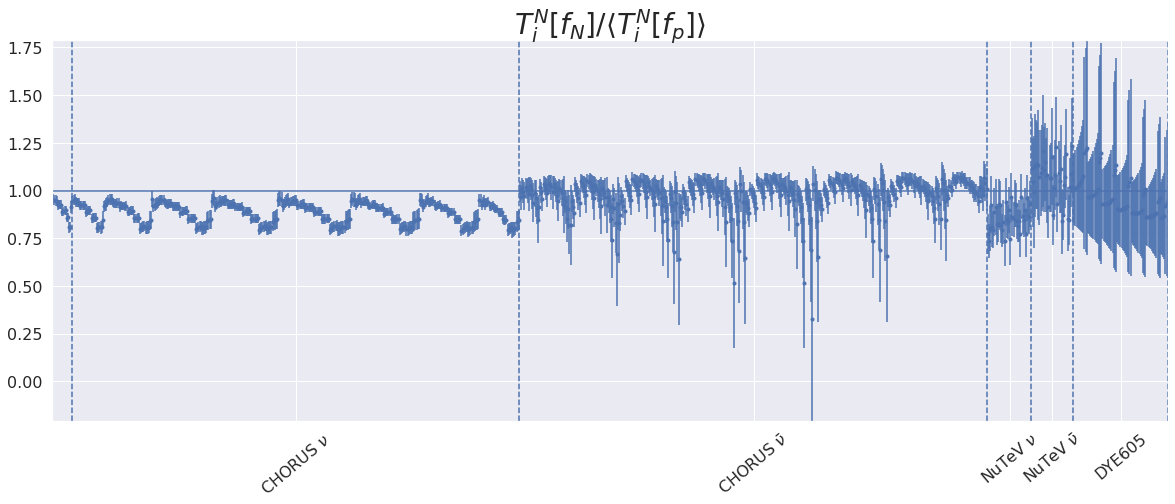
\includegraphics[width=\linewidth]{nuclear/plots/observable_ratio_nuclear.png}
   \caption{ Ratio between the nuclear observables computed with nPDFs, $T_i^N[f_N]$, and the central prediction computed with proton PDFs, $\langle T_i^N[f_p] \rangle$. The error is the standard deviation of the distribution of $T_i^N[f_N]$ replicas. Data are organised in bins of increasing $(x, Q^2)$ within each dataset. 
    \label{fig:nucobs} }
  \end{center}
\end{figure}
%%%%%%%%%%%%%%%%%%%%%%%%%%%%%%%%%%%%%%%%%%%%%%%%%%%%%%%%%%%%%%%%%%%%%%

Before proceeding to the covariance matrix itself, we can first investigate the change to the nuclear observables that arises from using nPDFs rather than proton ones. Fig.~\ref{fig:nucobs} shows the ratio of the observables calculated with nuclear PDFs to those with proton PDFs, for the heavy nuclear datasets. We can see in all datasets that there is a kinematic dependence, although this is especially evident in CHORUS. This is a result of the kinematic dependence of the ratio of proton and nuclear PDFs, which fits with the downwards turn at high $x$ expected from nuclear shadowing models. CHORUS $\nu$ and NuTeV $\nu$ data in particular show a systematic shift downwards which is not comfortably within errors. This suggests that applying a shift as well as an uncertainty could be a sensible strategy. 


\subsection{The heavy nuclear covariance matrix}
We now turn to the covariance matrix for heavy nuclear uncertainties. Fig.~\ref{fig:nuccov1} shows the square roots of the diagonal elements of this covariance matrix, which are equivalent to the \% per-point uncertainties. 
%%%%%%%%%%%%%%%%%%%%%%%%%%%%%%%%%%%%%%%%%%%%%%%%%%%%%%%%%%%%%%%%%%%%%
\begin{figure}[h]
  \begin{center}
    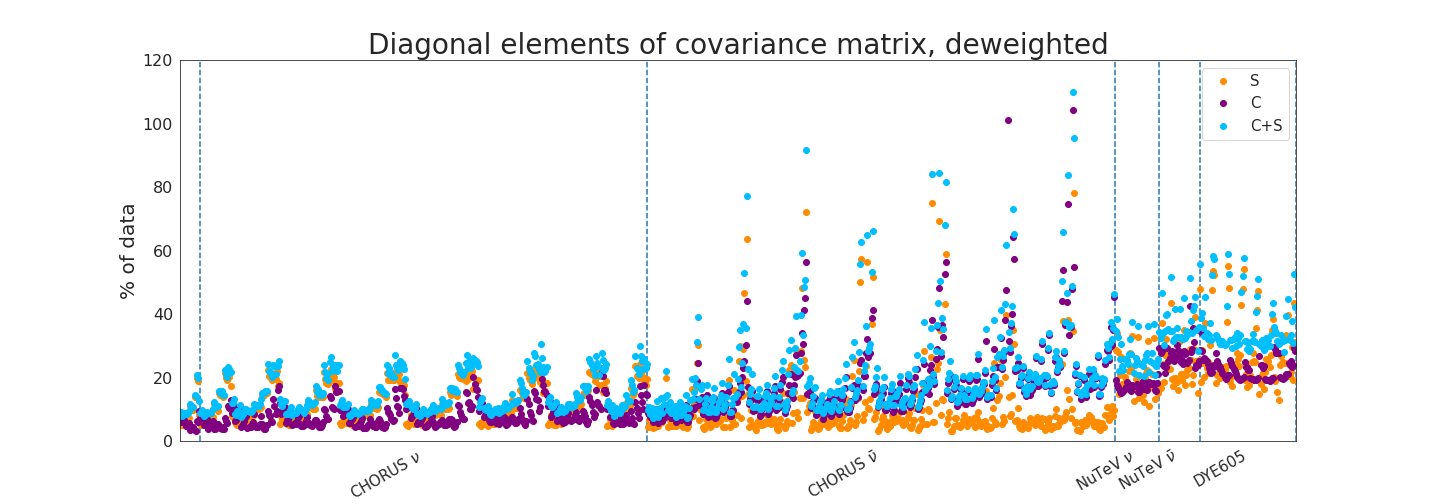
\includegraphics[width=\linewidth, trim={4cm 0 4cm 0}]{nuclear/plots//diag_covmat_deweighted.png}
        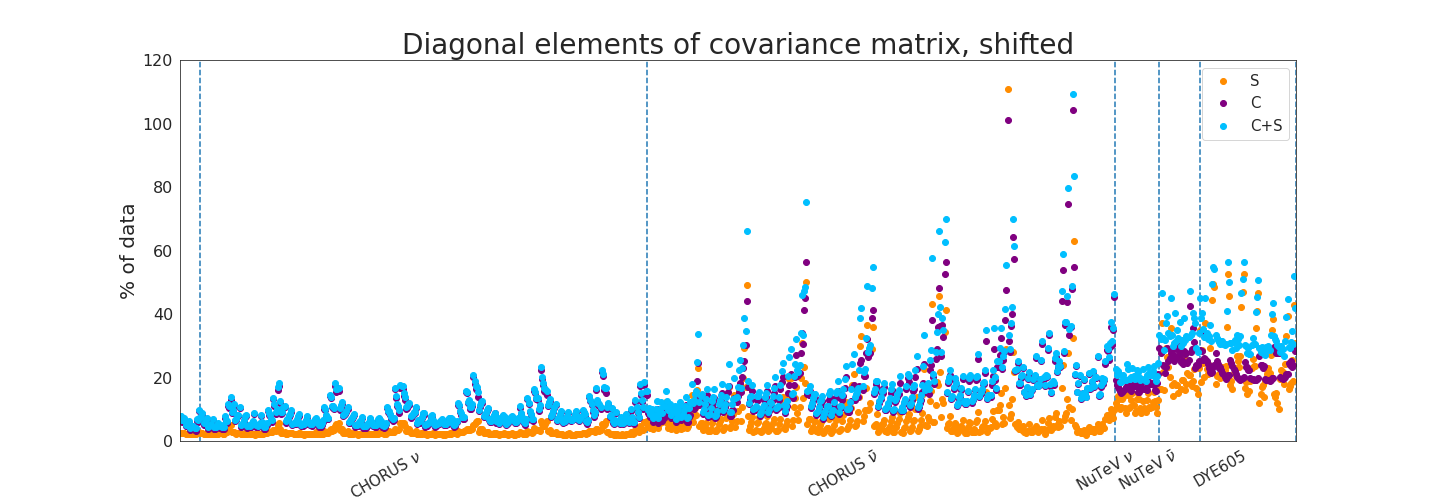
\includegraphics[width=\linewidth, trim={4cm 0 4cm 0}]{nuclear/plots/diag_covmat_shifted.png}
    \caption{Square root of diagonal elements of covariance matrices for $C$ (purple), $S$ (orange) and $C+S$ (blue). All values are displayed as a \% of data. Top: deweighted; bottom: shifted.
    \label{fig:nuccov1} }
    \end{center}
\end{figure}   
%%%%%%%%%%%%%%%%%%%%%%%%%%%%%%%%%%%%%%%%%%%%%%%%%%%%%%%%%%%%%%%%%%%%%
For the deweighted case, it is clear that the heavy nuclear uncertainties are comparable to the experimental uncertainties and are larger in most regions other than CHORUS $\bar{\nu}$. This suggests that all datasets apart from that will be significantly deweighted in the fit. We see that the plot has many features in common with Fig.~\ref{fig:nucobs}, in particular the kinematic pattern, and this makes sense as the covariance matrix is composed using the difference in observables when using nPDFs versus proton ones. For the shifted case, we see a marked decrease in the diagonal of $S$, such that nuclear per-point uncertainties seem no longer significant for CHORUS.
 
 %%%%%%%%%%%%%%%%%%%%%%%%%%%%%%%%%%%%%%%%%%%%%%%%%%%%%%%%%%%%%%%%%%%%%% 
\begin{figure}[h]
  \begin{centering} 
  \hspace{2cm}
    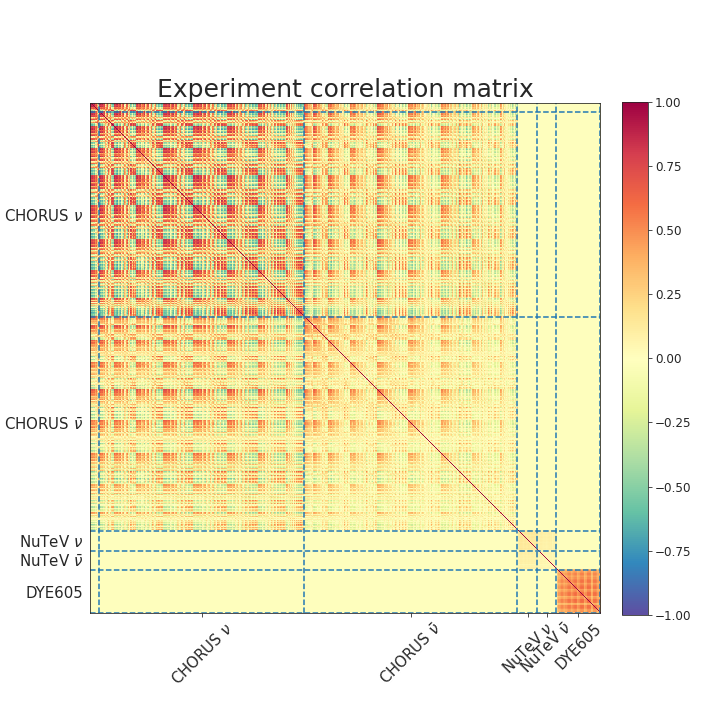
\includegraphics[width=0.45\linewidth, trim=0 1cm 0 1cm]{nuclear/plots/covmats_Experiment_nuclear.png}
    \newline
    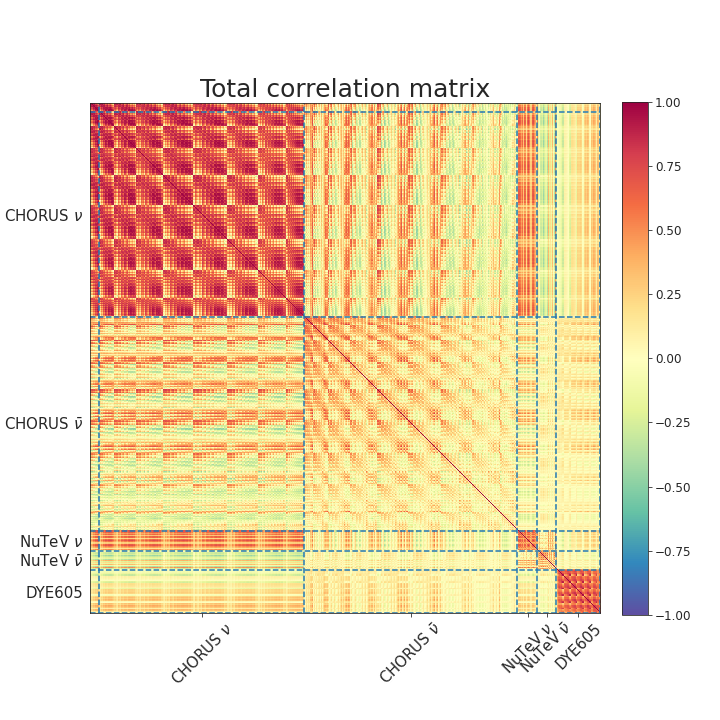
\includegraphics[width=0.45\linewidth]{nuclear/plots/covmats_Total_nuclear.png}
    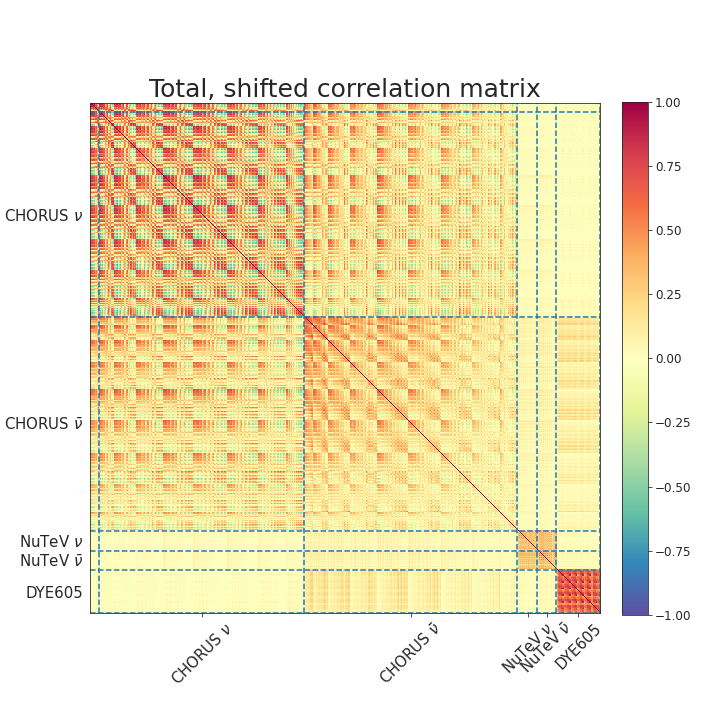
\includegraphics[width=0.45\linewidth]{nuclear/plots/covmats_Total_shifted_nuclear.png}
   \caption{ Correlation matrices for heavy nuclear data. The experiment correlation matrix, $C$, is shown above the total correlation matrices, $C+S$, for both the deweighted (left) and the shifted (right) case.
    \label{fig:nuccov} }
  \end{centering}
\end{figure}
%%%%%%%%%%%%%%%%%%%%%%%%%%%%%%%%%%%%%%%%%%%%%%%%%%%%%%%%%%%%%%%%%%%%%%

Fig.~\ref{fig:nuccov} investigates the pattern of correlations, displaying correlation matrices as defined in Sec.~\ref{sec:results} of Chapter~\ref{chapter:mhous}. Note that in \cite{Ball:2018twp} we considered covariance matrices experiment by experiment (a conservative approach), but here we compute the full heavy nuclear covariance matrix, including correlations between experiments. We display the correlation matrices for both the deweighted and shifted theory covariance matrices. Adding the theory covariance matrix introduces correlations on the off-block diagonals in both cases, but these are particularly strong in the deweighted case. CHORUS $\nu$ shows especially larger correlations upon introducing the deweighted $S$, but these are reduced almost to experiment level when the shifted $S$ is used instead. This is a clear consequence of the systematic shift in Fig.~\ref{fig:nucobs}, which is larger than the uncertainty from the nPDF. Once again, this is evidence that using the shifted formulism could be an appropriate choice.

\section{Deuteron uncertainties}
\label{sec:deutunc}
We now turn to uncertainties from deuteron data. The logic is the same as for heavy nuclear uncertainties, except we have a lot more deuteron data than heavy nuclear data from a particular element. This allows us to fit our own deuteron PDFs within the NNPDF methodology, resulting in NNLO PDFs to calculate uncertainties rather than NLO ones. 

The whole procedure is outlined in Fig.~\ref{fig:flowchart}. We split the global data into ``proton" and ``deuteron" data, where the proton data in fact include the heavy nuclear data considered in the previous section; this allows us to focus purely on deuteron uncertainties. The deuteron data are a combination of ``pure" deuteron data, coming from deuteron-only targets (SLAC and BCDMS), and ``mixed" deuteron data, which are ratios so depend also on proton target data (NMC, DYE866/NuSea and DYE906/SeaQuest). We can denote the pure data as $T_i^d[f_d]$ and the mixed data as $T_i^d[f_d, f_p]$, indicating the additional dependence of the latter on the proton PDF.

In normal proton PDF fits any deuteron observable is calculated using the isoscalar PDF, 
\be
\label{eqn:iso}
f_s = \frac{1}{2} (f_p + f_n),
\ee
where $f_n$ is the neutron PDF, obtained under the assumption of isospin invariance (by swapping $u$ and $d$ quarks in $f_p$).
%%%%%%%%%%%%%%%%%%%%%%%%%%%%%%%%%%%%%%%%%%%%%%%%%%%%%%%%%%%%%%%%%%%%%
\begin{figure}[h]
  \begin{center}
    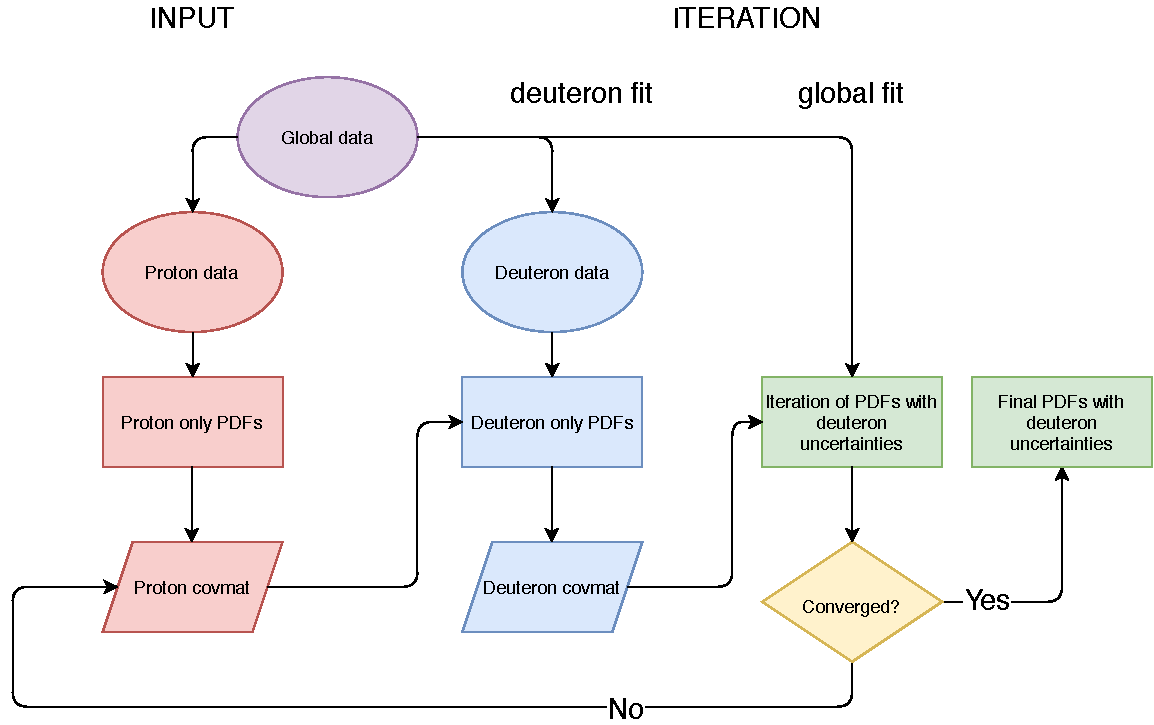
\includegraphics[width=\linewidth]{nuclear/plots/deut_flowchart.pdf}
   \caption{ Outline of the iterative procedure used to determine proton PDFs with deuteron uncertainties. The data are split into proton data and deuteron data. The proton data are used to find proton-only PDFs which are needed to fit deuteron observables in deuteron-only PDFs. These are used to construct a deuteron covariance matrix which is used in a global proton PDF fit. The whole process is iterated to consistency.
    \label{fig:flowchart} }
  \end{center}
\end{figure}
%%%%%%%%%%%%%%%%%%%%%%%%%%%%%%%%%%%%%%%%%%%%%%%%%%%%%%%%%%%%%%%%%%%%%%
The procedure is as follows:
\begin{enumerate}
\item The proton data are used to fit pure proton PDFs (uncontaminated by deuteron data), $\{f_p^{(k)}: k=1,\dots, N_{rep} \}$ with central value $f_p^{0} \equiv f_p$.
\item We cannot fit the pure deuteron PDFs without additional input because of the mixed ratio data ($T_i^d[f_d, f_p]$); these data require a proton PDF as input. We can use $f_p^{0}$ from the proton-only fit here, but since this is only the central value we must include a proton covariance matrix to account for the uncertainty due to the proton PDF. This is composed
\be 
\label{eq:protoncovmatrix}
\begin{split}
&S_{ij}^p = \langle \Delta_i^{p,\ (k)}, \Delta_j^{p,\ (k)} \rangle \\
&\Delta_i^{p,\ (k)} = T_i^d[f_d^{(0)}, f_p^{(k)}] - T_i^d[f_d^{(0)}, f_p^{(0)}],
\end{split}
\ee
where here $i$ runs over the deuteron ratio data only. This encapsulates the correlations between the ratio datasets due to their common dependence on the proton PDF.
\item Fit the deuteron PDFs using $C_{ij} + S^p_{ij}$ for the deuteron ratio data. However, in practice $S^p$ depends on $f_d^{(0)}$ and we don't know this yet (that's what we're trying to find!). To first approximation we can replace $f_d^{(0)} \to f_s^{(0)}$, using the isoscalar PDF from Eqn.~\ref{eqn:iso}. This is a reasonable exchange, given that $S_{ij}^p$ is a measure of uncertainty, and acts only to deweight data in the fit; using $f_s$ should have only a very small effect. In principle, we could then iterate this to consistency, using the output $f_d$ to determine a new $S_{ij}^p$ and perform a new deuteron fit. However we are less interested in determining the deuteron PDFs themselves, more in their application in creating a covariance matrix for fitting proton PDFs. Any (already small) effect from using $f_s$ in $S^p$ will become smaller when finding $f_d$ and then smaller again when finding $f_p$, where the only influence is via a covariance matrix which depends on $f_d$.
\item Use $f_d$ to generate a deuteron covariance matrix:
\be 
\label{eq:deuteroncovmatrix}
\begin{split}
&S_{ij}^d = \langle \Delta_i^{d,\ (k)}, \Delta_j^{d,\ (k)} \rangle \\
&\Delta_i^{d,\ (k)} = 
\begin{cases}
T_i^d[f_d^{(k)}] - T_i^d[f_s^{(0)}]  &i \in \text{pure} \\
T_i^d[f_d^{(k)}, f_p^{(0)}] - T_i^d[f_s^{(0)}, f_p^{(0)}] &i \in \text{mixed},
\end{cases}
\end{split}
\ee 
or, for the shifted case,
\be 
\label{eq:deuteronshifted}
\begin{split}
\Delta_i^{d,\ (k)} = 
\begin{cases}
T_i^d[f_d^{(k)}] - T_i^d[f_d^{(0)}]  &i \in \text{pure} \\
T_i^d[f_d^{(k)}, f_p^{(0)}] - T_i^d[f_d^{(0)}, f_p^{(0)}] &i \in \text{mixed}, \\
\end{cases}
\end{split}
\ee
\be
\begin{split}
\delta T_i^d = 
\begin{cases}
T_i^d[f_d^{(0)}] - T_i^d[f_s^{(0)}]  &i \in \text{pure} \\
T_i^d[f_d^{(0)}, f_p^{(0)}] - T_i^d[f_s^{(0)}, f_p^{(0)}] &i \in \text{mixed}.
\end{cases}
\end{split}
\ee
$S^d$ incorporates correlations between the deuteron data due to their common dependence on the deuteron PDF and, for the ratio data, their consequential dependence on proton PDFs.
\item Perform a global proton PDF fit incorporating $S^d$ for the deuteron data. These are PDFs with deuteron uncertainties included.
\item Use the resulting proton PDFs in place of the proton-only PDFs in Step 2, thus iterating the procedure. We expect this to converge rapidly for a few reasons: first, the influence of deuteron data in a proton fit is small; second, a small change in the proton PDF makes little difference to the deuteron uncertainty; third, the effect of deuteron uncertainties on the weight of data in the fit is anticipated to be small.
\end{enumerate}

\begin{table}[h]
  \centering
  \scriptsize
  \renewcommand{\arraystretch}{1.13}
  \begin{tabularx}{\textwidth}{lllX}
    \toprule
    {\bf Iteration }  & {\bf Dataset }            & {\bf Fit ID }        & { \bf Description }\\
    \midrule
    Baseline    & Proton and Deuteron & global-base    & NNPDF4.0 fit without nuclear uncertainties\\
    \midrule
    Iteration 0 & Proton              & proton-ite0    & Same as baseline, but restricted to the proton dataset\\
    \midrule
    Iteration 1 & Deuteron            & deuteron-ite1  & Same as baseline, but restricted to the deuteron dataset
                                                         and supplemented with a proton covariance matrix determined
                                                         from the proton-ite0 fit according to
                                                         Eqn.~\ref{eq:protoncovmatrix}.\\
                & Proton and Deuteron & global-ite1-dw & Same as baseline, but supplemented with a deuteron covariance
                                                         matrix determined from the deuteron-ite1 fit according to
                                                         Eqn.~\ref{eq:deuteroncovmatrix}.\\
    \midrule
    Iteration 2 & Deuteron            & deuteron-ite2  & Same as deuteron-ite1, but with a proton covariance matrix
                                                         determined from the global-ite1-dw fit.\\
                & Proton and Deuteron & global-ite2-dw & Same as global-ite1-dw, but with a deuteron covariance matrix
                                                         determined from the deuteron-ite2 fit.\\
                & Proton and Deuteron & global-ite2-sh & Same as global-ite2-sh, but with a deuteron covariance matrix
                                                         and shifts determined according to
                                                         Eqn.~ref{eq:deuteronshifted}.\\
    \bottomrule
  \end{tabularx}
  \caption{A summary of the fits performed in this study, see text for details.}
  \label{tab:fits}
\end{table}


Note that once again in this procedure we are not double counting the deuteron data; we use them once to determine the deuteron uncertainty and once to do a global fit to find the proton PDFs. Adding uncertainties actually makes the deuteron data count \textit{less}.

The fits performed are summarised in Tab.~\ref{tab:fits}. The baseline fit, global-base, is the baseline fit for NNPDF4.0~\cite{EmanueleTalk} without nuclear uncertainties included (the uncertainties we determine in this Chapter will be included in the final NNPDF4.0 release). We determine a proton-only fit in what we term ``Iteration 0", and then perform two iterations of determining the deuteron and global proton fits, termed ``Iteration 1" and ``Iteration 2". 
%%%%%%%%%%%%%%%%%%%%%%%%%%%%%%%%%%%%%%%%%%%%%%%%%%%%%%%%%%%%%%%%%%%%%
\begin{figure}[h]
  \begin{center}
    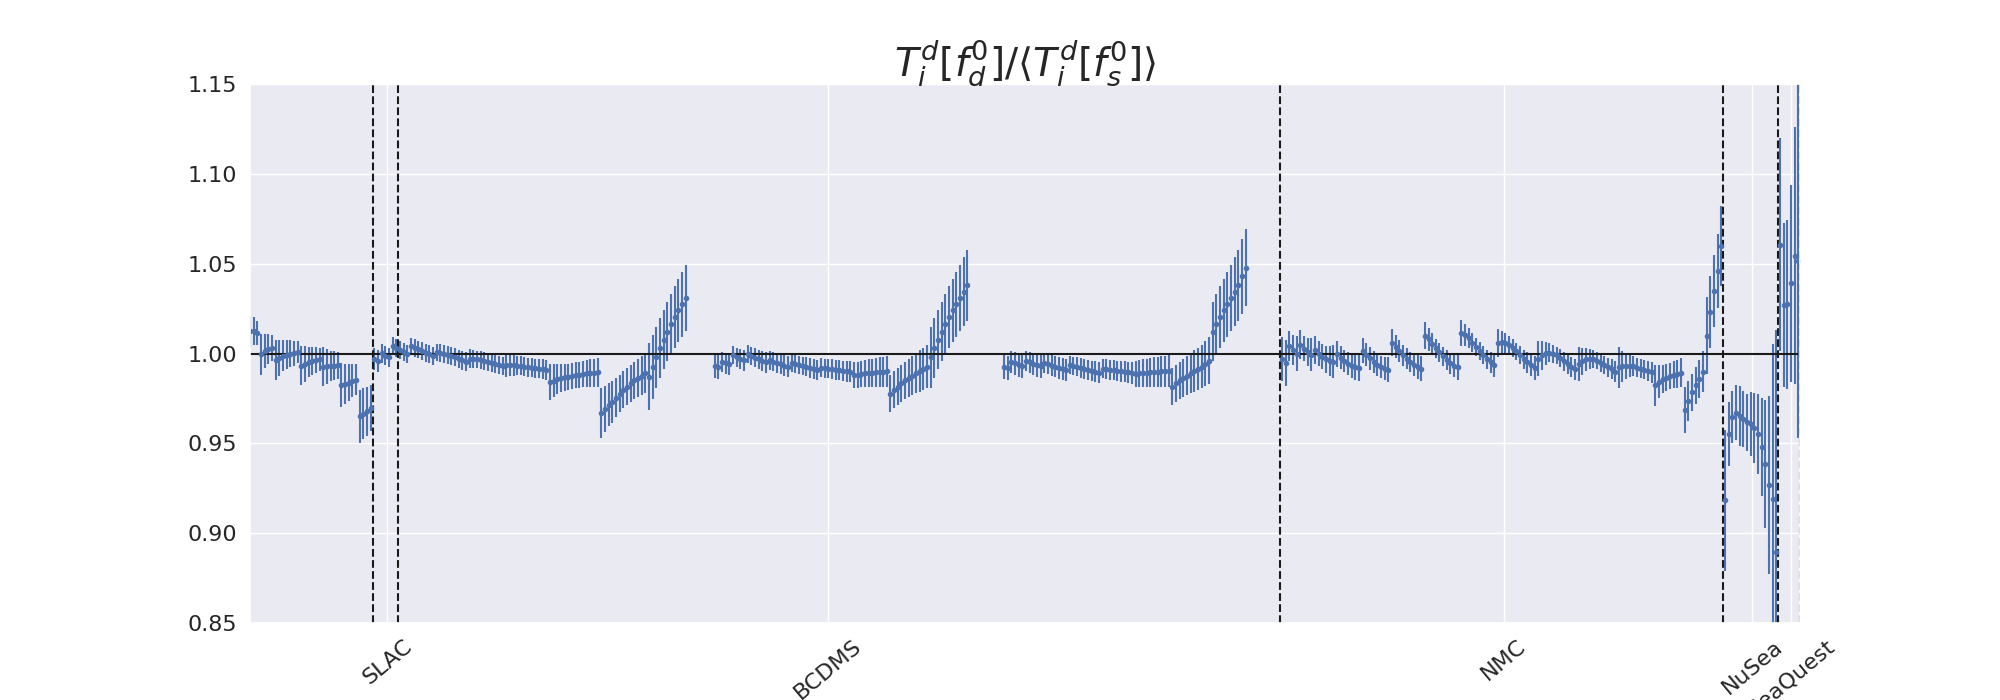
\includegraphics[width=\linewidth, trim={4cm 0 4cm 0}]{nuclear/plots/observable_ratio_updated.png}
   \caption{ Like Fig.~\ref{fig:nucobs} but for deuteron observables. Ratio between the deuteron observables computed with Iteration 1 deuteron PDFs, $T_i^d[f_d]$, and the central prediction computed with the isoscalar PDF, $\langle T_i^d[f_s] \rangle$. The error is the standard deviation of the distribution of $T_i^d[f_d]$ replicas. Data are organised in bins of increasing $(x, Q^2)$ within each dataset. 
    \label{fig:deutobs} }
  \end{center}
\end{figure}
%%%%%%%%%%%%%%%%%%%%%%%%%%%%%%%%%%%%%%%%%%%%%%%%%%%%%%%%%%%%%%%%%%%%%%

As in the case for heavy nuclear data, it is useful to first look at the effect on the deuteron observables of using the deuteron PDF rather than the proton one (Fig.~\ref{fig:deutobs}). The uncertainties are quite large but the ratio of observables is consistent with 1 in most regions other than high $x$, where nuclear shadowing is expected to play a part leading to large negative corrections. This mirrors what was seen in the heavy nuclear case (Fig.~\ref{fig:nucobs}). The observables for NuSea show a systematic offset outwith uncertainties, like what we saw for CHORUS and NuTeV $\nu$.

\subsection{The deuteron covariance matrix}
We now go on to investigate the deuteron covariance matrix. The diagonal elements are displayed in Fig.~\ref{fig:deutcov}. Again, we see a pattern that parallels the pattern in the deuteron observable ratios; the size of the per-point uncertainty depends on the kinematics. 
%%%%%%%%%%%%%%%%%%%%%%%%%%%%%%%%%%%%%%%%%%%%%%%%%%%%%%%%%%%%%%%%%%%%%
\begin{figure}[H]
  \begin{center}
      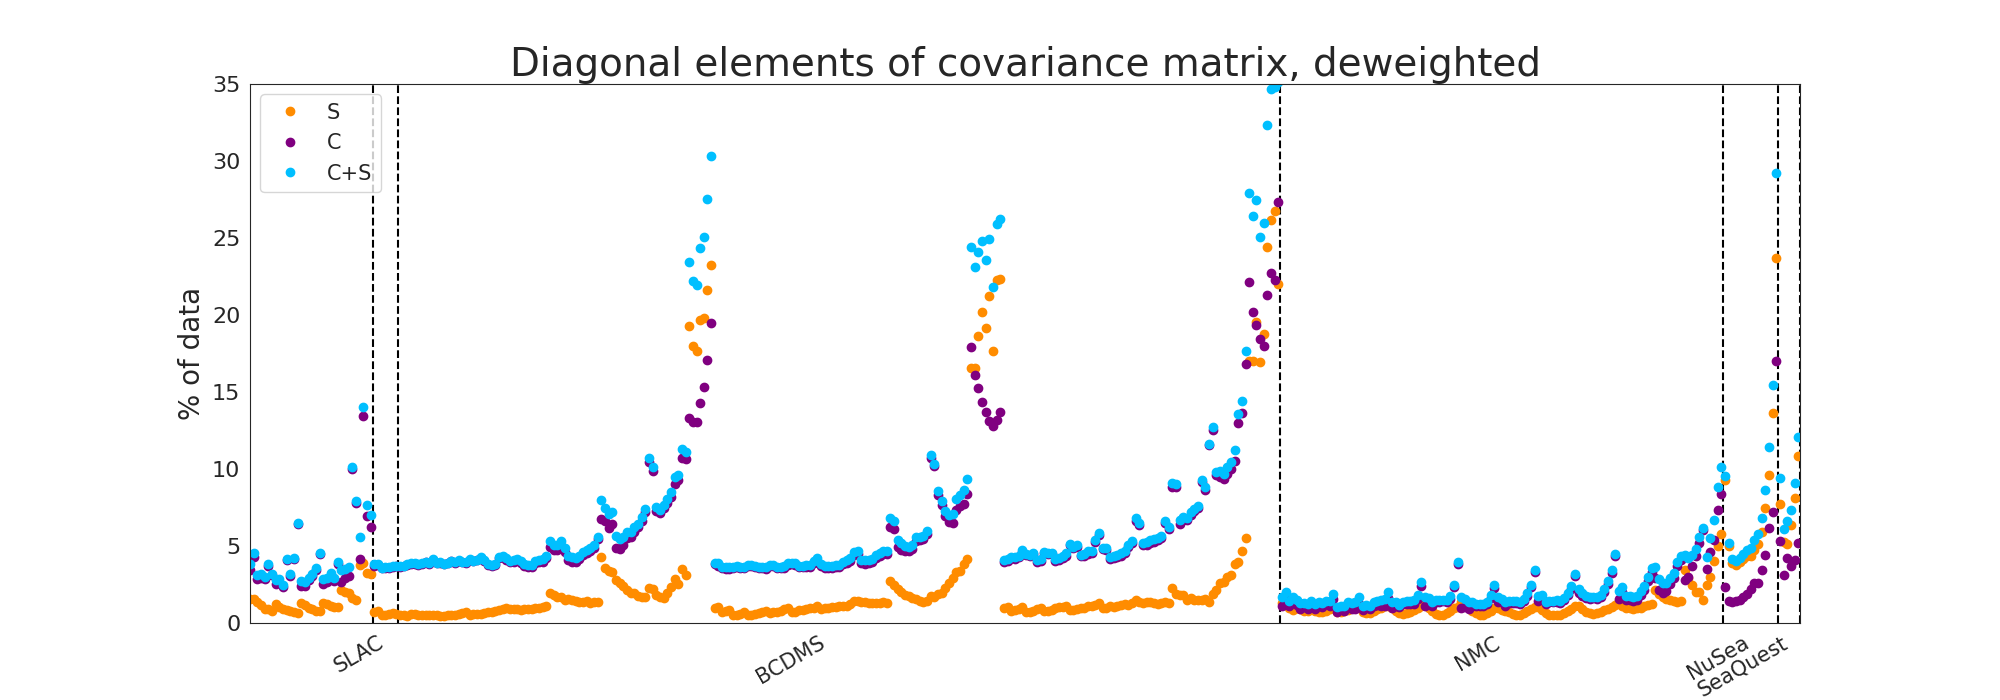
\includegraphics[width=\linewidth, trim={4cm 0 4cm 0}]{nuclear/plots/diag_covmat_updated.png}
    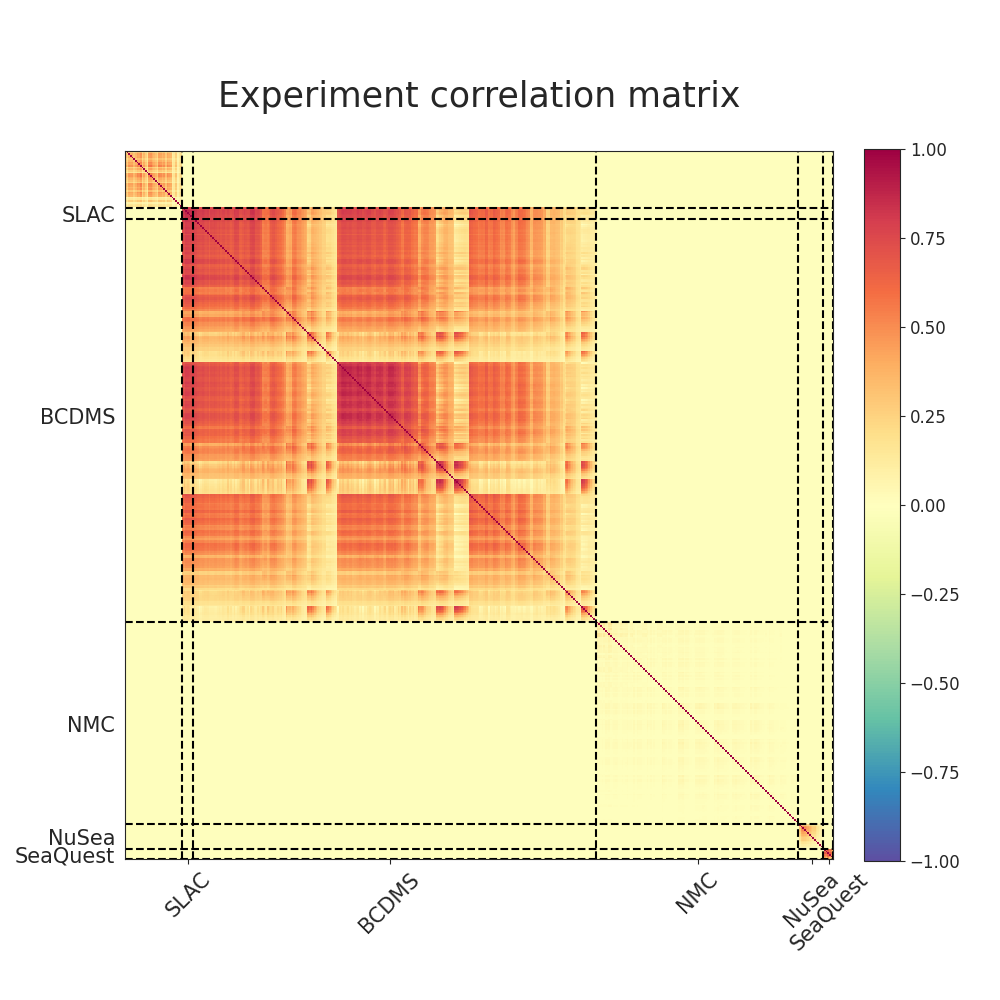
\includegraphics[width=0.45\linewidth]{nuclear/plots/expcov_updated.png}
        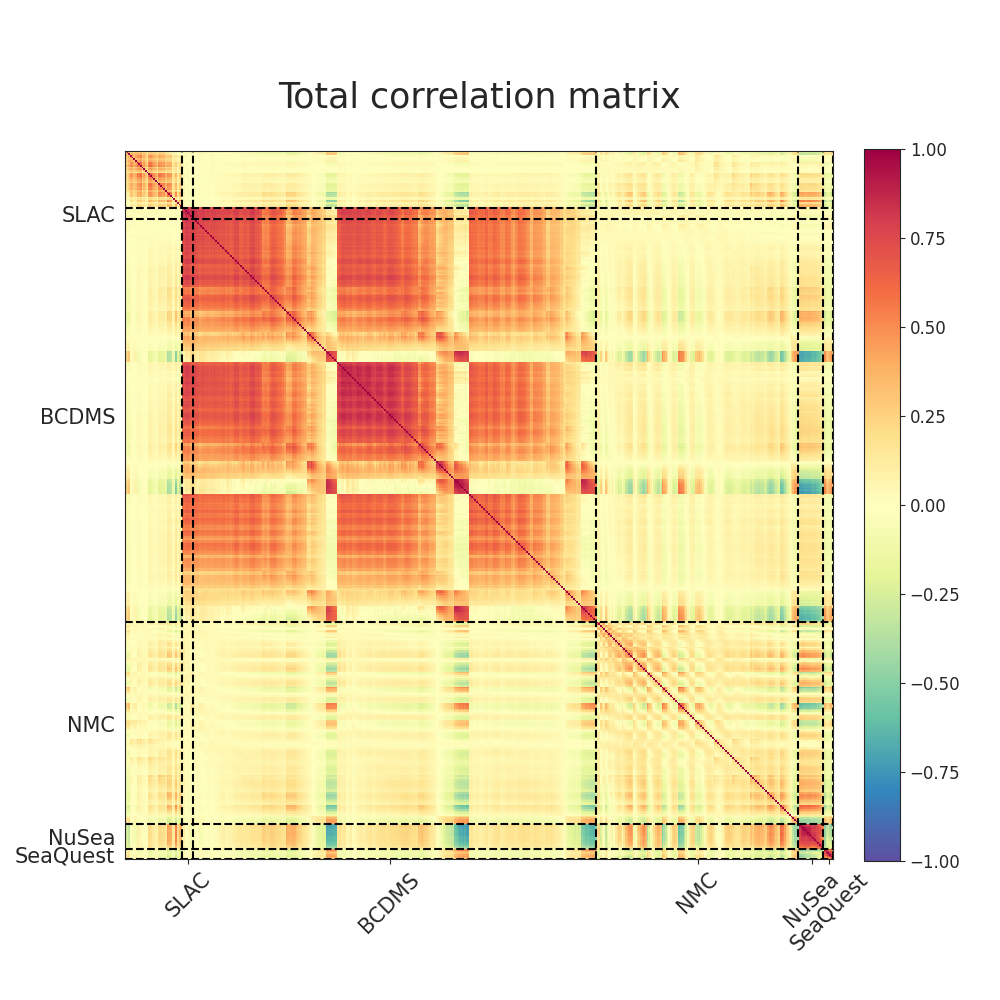
\includegraphics[width=0.45\linewidth]{nuclear/plots/totcov_updated.png}
    \caption{\textbf{Top panel:} Square root of diagonal elements of covariance matrices for $C$ (purple), $S$ (deweighted; orange) and $C+S$ (deweighted; blue). All values are displayed as a \% of data. \textbf{Bottom panel: }Correlation matrices. $C$ (left) and $C+S$ (deweighted; right). The deweighted case only is displayed, but the qualitative features remain the same for the shifted case.
    \label{fig:deutcov} }
    \end{center}
\end{figure}   
%%%%%%%%%%%%%%%%%%%%%%%%%%%%%%%%%%%%%%%%%%%%%%%%%%%%%%%%%%%%%%%%%%%%%
The deuteron uncertainty is smaller than the experimental uncertainty for the  pure deuteron datasets (SLAC and BCDMS), but is comparable for the mixed ratio data (NMC, NuSea and SeaQuest). This is because ratio data have smaller experimental uncertainties due to a significant cancellation of systematic errors. The bottom part of the figure shows the full matrix plots. As above, we see the most impact is on the ratio data. The figures show only the deweighted case, but this is qualitatively similar to the shifted case. 

\subsection{Deuteron correction factor}

As an additional investigation, we can use the fitted deuteron PDFs to evaluate a correction to $F_2$ by computing the ratio $F_2^d/F_2^p$. This can then be compared to the result from nNNPDF2.0 and to the parametric correction used in MSHT20~\cite{Bailey:2020ooq}, which is based on four fitted parameters. 
%%%%%%%%%%%%%%%%%%%%%%%%%%%%%%%%%%%%%%%%%%%%%%%%%%%%%%%%%%%%%%%%%%%%%
\begin{figure}[H]
  \begin{center}
      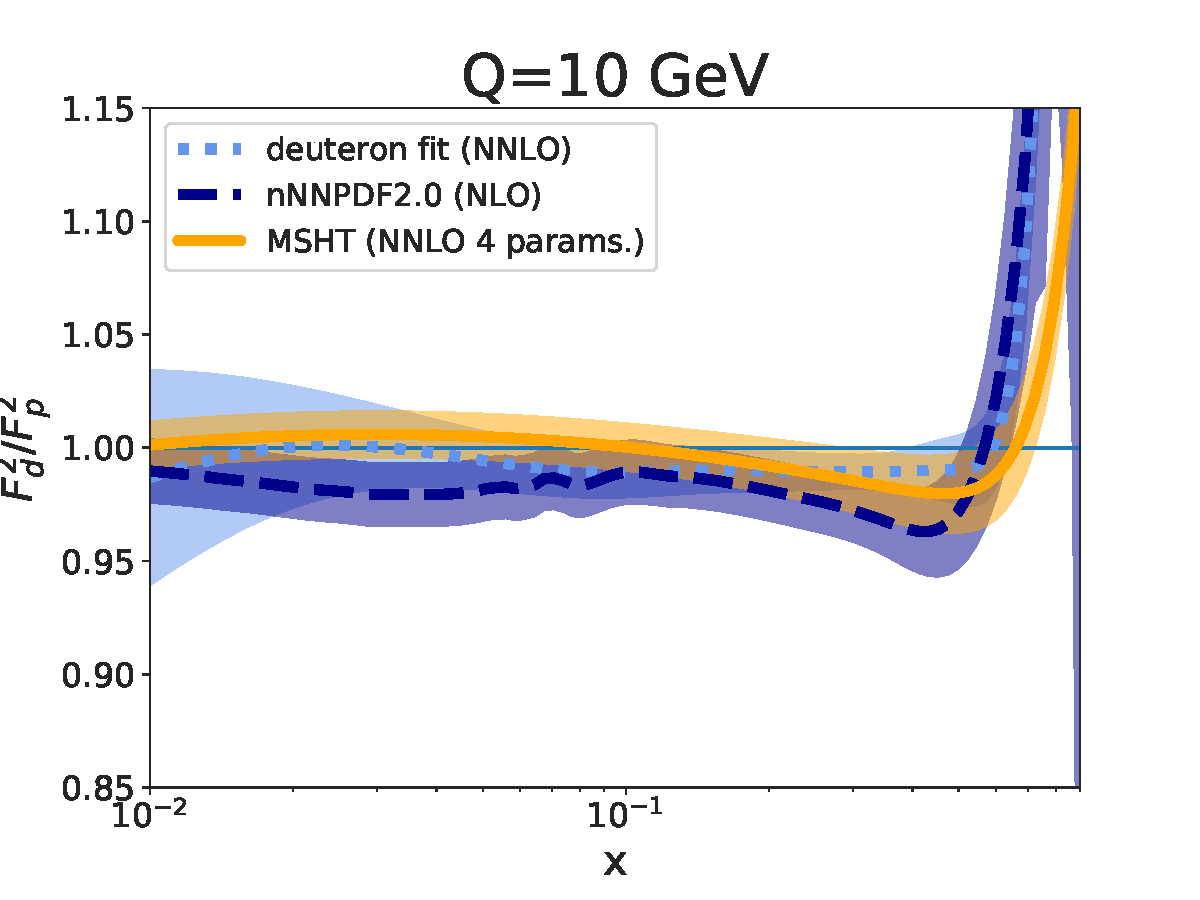
\includegraphics[width=0.8\linewidth]{nuclear/plots/newdeut_10.pdf}
    \caption{$F_2^d/F_2^p$ evaluated using deuteron PDFs from the present determination (deuteron-ite2), deuteron PDFs from nNNPDF2.0, and via the model correction used in MSHT20 fits.
    \label{fig:deutpdfcomp} }
    \end{center}
\end{figure}   
%%%%%%%%%%%%%%%%%%%%%%%%%%%%%%%%%%%%%%%%%%%%%%%%%%%%%%%%%%%%%%%%%%%%%
This comparison can be seen in Fig.~\ref{fig:deutpdfcomp} at $Q$ = 10 GeV. From this, deuteron correction to the structure function is clearly small, just a few percent across the whole of $x$. The shape of the distribution also fits that expected from nuclear shadowing, with a dip at large $x$. All three determinations agree within uncertainties, giving us confidence in the robustness of our procedure. They also all have uncertainties of a similar size, despite the fact that nNNPDF2.0 is only at NLO. This is because it also contains heavy nuclear data through the constraint of continuity of $A/Z$. The uncertainty for the deuteron fit at NNLO is slightly larger at low $x$ in the non-data region, reflecting the more conservative determination with no model dependence or continuity constraints imposed. 

\section{PDFs with nuclear uncertainties}
\label{sec:nucpdfs}
Having constructed and studied deuteron and heavy nuclear uncertainties, we can then include them in fits. Table~\ref{tab:fits-unc} summarises the various configurations of nuclear uncertainties and shifts. The NNPDF4.0 release includes (deweighted) deuteron and heavy nuclear uncertainties as a default, so it serves as the baseline for comparison.
\begin{table}[h]
  \centering
  \scriptsize
  \renewcommand{\arraystretch}{1.13}
  \begin{tabularx}{0.8\textwidth}{lX}
    \toprule
    {\bf Fit label }     & { \bf Description }\\
    \midrule
    NNPDF4.0    & Baseline fit from NNPDF4.0 \\
    No nuclear data & Without nuclear datasets \\
    No nuclear unc. & Without nuclear uncertainties \\
    Heavy nuclear unc. & Heavy nuclear uncertainties only \\
    Heavy nuclear shifted & Heavy nuclear uncertainties with shifted central value \\
    Deuteron unc. & Deuteron uncertainties only \\
    Deuteron shifted & Deuteron uncertainties with shifted central value \\
    Shifted & (All) nuclear uncertainties with shifted central value \\  
    \bottomrule
  \end{tabularx}
  \caption{A summary of the fits with different treatments of nuclear data.}
  \label{tab:fits-unc}
\end{table}

\begin{table}[h]
  \centering
  \scriptsize
  \renewcommand{\arraystretch}{1}
  \begin{tabularx}{\textwidth}{l|l|lll|lll}
    \toprule
   & No nuc unc   & Deut unc & Heavy nuc unc & {\bf NNPDF4.0 } & Deut shift  & Heavy nuc shift & Shifted   \\
   \midrule
 {\bf $\chi^2$ } & 1.269 & 1.257 & 1.193 & {\bf 1.162 }  & 1.244  & 1.196 & 1.166  \\
 {\bf $\phi$ } & 0.160 & 0.158 & 0.160   & {\bf 0.164} & 0.158  &  0.170 & 0.169\\
    \bottomrule
  \end{tabularx}
  \caption{Total $\chi^2$ and $\phi$ values for nuclear data sets for the various fits. \label{tab:totchi2} }
  
\end{table}

% $\pm$ 0.006
% $\pm$ 0.006
% $\pm$ 0.007
% $\pm$ 0.005
% $\pm$ 0.005
% $\pm$ 0.005
% $\pm$ 0.005


Table~\ref{tab:totchi2} gives the total $\chi^2$ and $\phi$ values for these fits, where $\phi$ is defined
\begin{equation}
\phi \equiv \sqrt{\langle \chi^2[T] \rangle - \chi^2[\langle T \rangle ]},
\end{equation}
where $T$ are the theoretical predictions and $\langle \cdot \rangle$ denotes the average over PDF replicas. In \cite{Ball:2014uwa} it is shown that this gives the ratio of uncertainties after fitting to the uncertainties of the original data, averaged over data points. The partial values per nuclear dataset can be seen in Fig.~\ref{fig:chi2phi}. Overall, including nuclear uncertainties causes the $\chi^2$ to drop from 1.27 to 1.16, indicating a substantially better fit quality. This is to be expected, seeing as we are adding an uncertainty into the fit, accompanied by an increase in $\phi$. The NNPDF4.0 baseline gives the best fit, which is dominated by the inclusion of heavy nuclear uncertainties without a shift. The impact at the nuclear dataset level is striking, with a significant improvement in both $\chi^2$ and $\phi$ for most of these datasets. The difference between the deweighted and shifted prescriptions, however, is minimal.
%%%%%%%%%%%%%%%%%%%%%%%%%%%%%%%%%%%%%%%%%%%%%%%%%%%%%%%%%%%%%%%%%%%%%
\begin{figure}[H]
  \begin{center}
      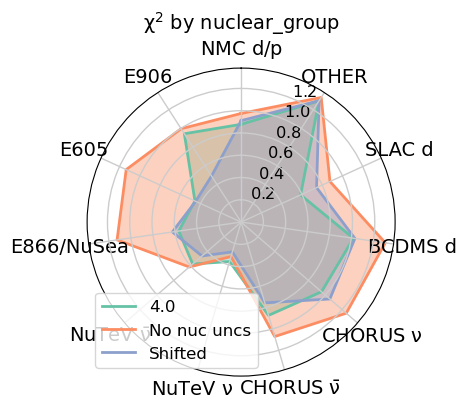
\includegraphics[width=0.3\linewidth, trim={0 0 0 1cm}]{nuclear/plots/spiderchi2_3_new.png}
    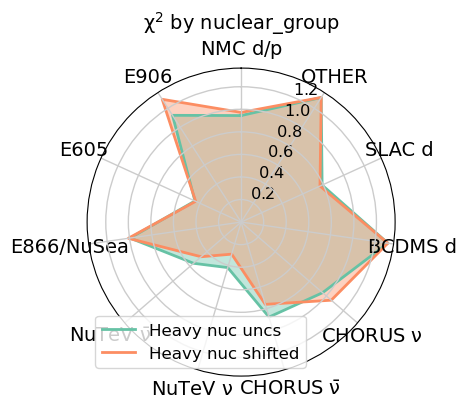
\includegraphics[width=0.3\linewidth, trim={0 0 0 0}]{nuclear/plots/spiderchi2_2_new.png}
        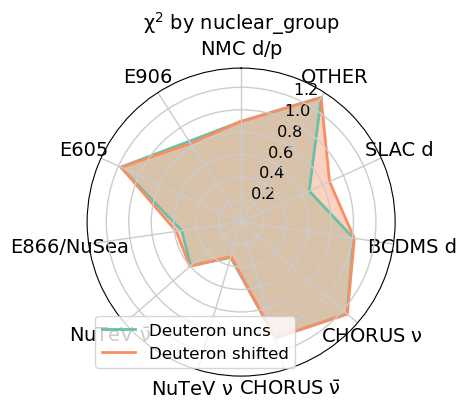
\includegraphics[width=0.3\linewidth, trim={0 0 0 0}]{nuclear/plots/spiderchi2_1_new.png}
      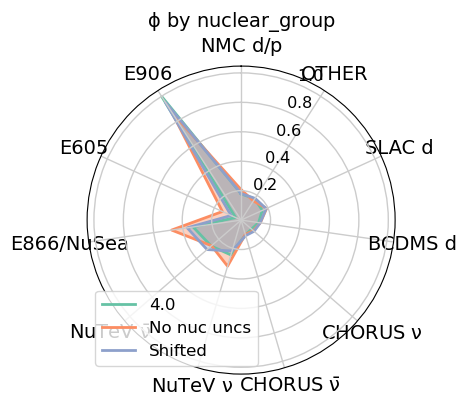
\includegraphics[width=0.3\linewidth, trim={0 0cm 0 0cm}]{nuclear/plots/spiderphi_3_new.png}
    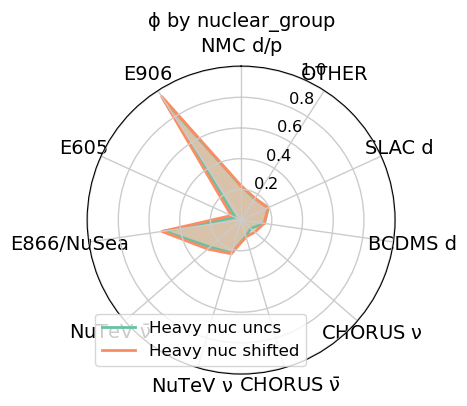
\includegraphics[width=0.3\linewidth]{nuclear/plots/spiderphi_2_new.png}
        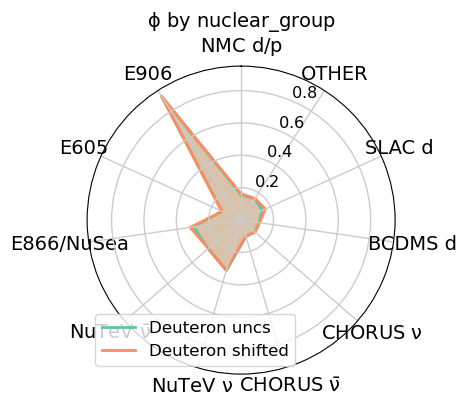
\includegraphics[width=0.3\linewidth, trim={0 0cm 0 0}]{nuclear/plots/spiderphi_1_new.png}
    \caption{Partial $\chi^2$ (top row) and $\phi$  (bottom row) values broken down by nuclear dataset for the different configurations of uncertainties. All other datasets are collected under OTHER. 
    \label{fig:chi2phi} }
    \end{center}
\end{figure}   
%%%%%%%%%%%%%%%%%%%%%%%%%%%%%%%%%%%%%%%%%%%%%%%%%%%%%%%%%%%%%%%%%%%%%
%%%%%%%%%%%%%%%%%%%%%%%%%%%%%%%%%%%%%%%%%%%%%%%%%%%%%%%%%%%%%%%%%%%%%
\begin{figure}[H]
  \begin{center}
      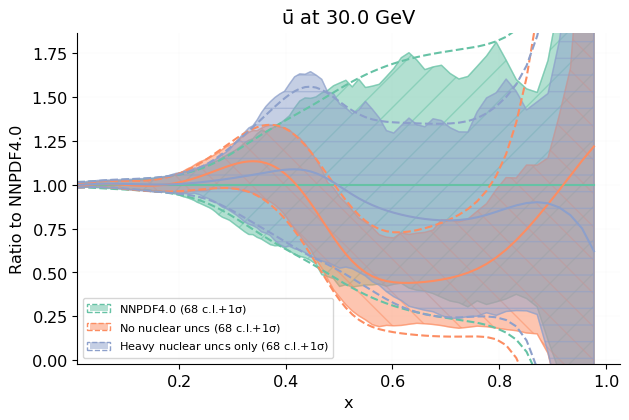
\includegraphics[width=0.49\linewidth]{nuclear/plots/ubar1.png}
     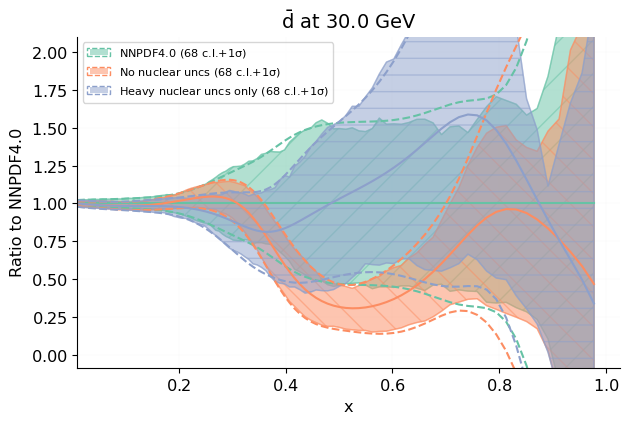
\includegraphics[width=0.49\linewidth]{nuclear/plots/dbar1.png}
    \caption{Impact of including nuclear uncertainties in NNPDF4.0. The default (green) is to include them for all nuclear data. Fits with no nuclear uncertainties (orange) and with only heavy nuclear uncertainties (blue) are also shown.
    \label{fig:pdfs1} }
    \end{center}
\end{figure}   
%%%%%%%%%%%%%%%%%%%%%%%%%%%%%%%%%%%%%%%%%%%%%%%%%%%%%%%%%%%%%%%%%%%%%

It's also helpful to look at the PDFs themselves. Nuclear uncertainties have an effect which is important in the large $x$ region, where the nuclear data are. Firstly, we would like to know what impact adding nuclear uncertainties has on the PDFs. In Fig.~\ref{fig:pdfs1} we compare NNPDF4.0 to the fit without nuclear uncertainties. Including nuclear uncertainties causes a significant change to the shape of the PDFs in the large $x$ region. This corresponds to the nuclear shadowing region, where nPDFs are lower compared to proton ones. Having no nuclear uncertainties causes the PDFs to be pulled downwards in this region, in the direction of the nPDFs.

Also displayed in Fig.~\ref{fig:pdfs1} is a fit with only heavy nuclear uncertainties. It is clear that heavy nuclear uncertainties are responsible for the bulk of the impact, which is expected given the impact at the data level is more significant for thcese data (see Figs.~\ref{fig:nuccov1} and ~\ref{fig:deutcov}).
%%%%%%%%%%%%%%%%%%%%%%%%%%%%%%%%%%%%%%%%%%%%%%%%%%%%%%%%%%%%%%%%%%%%%
\begin{figure}[H]
  \begin{center}
      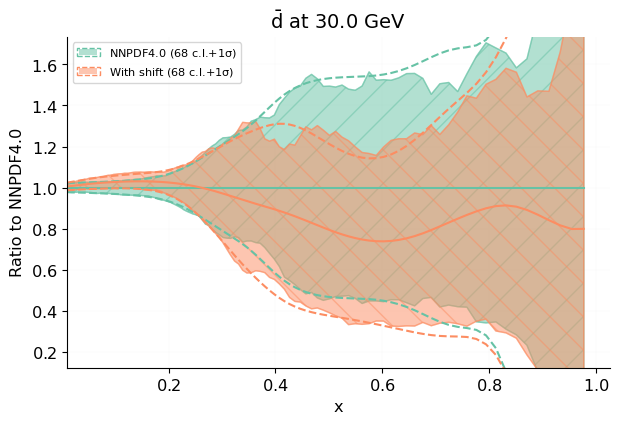
\includegraphics[width=0.49\linewidth]{nuclear/plots/shiftvdw_pdfplot.png}
     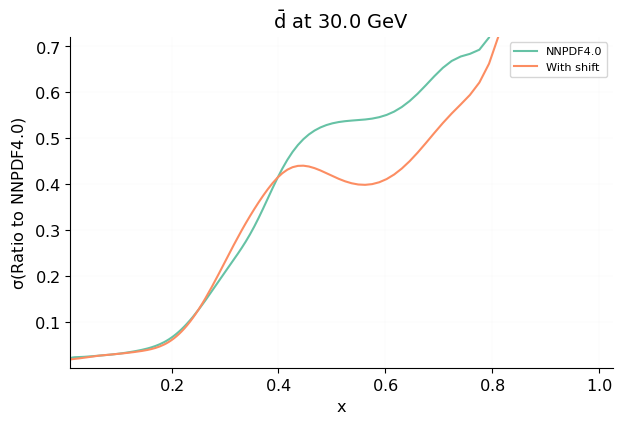
\includegraphics[width=0.49\linewidth]{nuclear/plots/shiftvdw_errplot.png}
    \caption{The impact of shifting (orange) versus deweighting (green) for the $\bar{d}$ distribution. The right panel shows the uncertainties for clarity. The effects on the $\bar{u}$ distribution are qualitatively similar. 
    \label{fig:pdfs3} }
    \end{center}
\end{figure}   
%%%%%%%%%%%%%%%%%%%%%%%%%%%%%%%%%%%%%%%%%%%%%%%%%%%%%%%%%%%%%%%%%%%%%
Secondly, we would like to look at what happens when we also apply a shift to the nuclear data, following Eqn.~\ref{eqn:shiftnuc}. This can be seen in Fig.~\ref{fig:pdfs3} for the $\bar{d}$ distribution. There is a clear reduction of PDF uncertainties when using the shifted prescription versus the deweighted prescription. However, as we saw before, there is little impact at the level of $\chi^2$ and $\phi$ values, and the two outcomes are equivalent within uncertainties. From this we see that choosing one of these approaches over the other will not have a great impact. When making the choice of approach, we note that the shift is calculated relative to the value with proton PDFs, and so is itself dependent on the proton PDFs. This opens up the risk of double counting, and so the shift must be treated with caution. Adding uncertainties, however, always decreases the weight of data points, and so the deweighted prescription is the most conservative. Given also that it leads to a slightly lower total $\chi^2$ and $\phi$, we will opt to use the deweighted prescription in NNPDF4.0; including only an uncertainty for both deuteron and heavy nuclear data.

\section{Summary}
Nuclear data are important in PDF fits, but effects due to the nuclear environment are hard to quantify. To bring PDFs to 1\% accuracy, we need  to address these ``small" but nevertheless important differencecs. We used the theory covariance matrix formalism outlined in Chapter~\ref{chapter:thuncs} to include nuclear uncertainties in the next generation PDF fits. We adopted an empirical approach by recalculating predictions for nuclear observables with nuclear PDFs and using the shifts in predictions to construct a nuclear covariance matrix. 

We analysed deuteron and heavy nuclear data separately, using nNNPDF2.0 for heavy nuclear PDFs, and fitting deuteron PDFs using an iterative procedure in the NNPDF3.1 methodology. The resulting uncertainties are a crucial ingredient in the latest release, NNPDF4.0. They lead to a reduced global $\chi^2$ and the relaxation of tension between the nuclear DIS and LHC DY data. Including the uncertainties causes a modest shift in the central value of PDFs and an increase in errors, in the high $x$ nuclear data region. This difference is driven by the heavy nuclear data. We also investigated a procedure to shift the nuclear predictions, which was equivalent within uncertainties to including only an uncertainty, but with a slightly higher global $\chi^2$ and smaller PDF uncertainties. We opt to include uncertainties without a shift in NNPDF4.0.


\label{sec:summandoutlook}

\chapter{Deuteron Uncertainties - 0\%}
%\chapter{Higher Twist Uncertainties - 0\%}
\section{The role of higher twist data in PDFs}
\section{Ansatz for a higher twist correction}
\section{Using a neural network to model higher twist}
\subsection{Model architecture}
\subsection{Training and validating the neural network}
\section{Form of the higher twist correction}
\section{The higher twist covariance matrix}
\section{PDFs with higher twist uncertainties}
\chapter{Conclusion}

In this thesis we have considered uncertainties in the theoretical predictions that go into PDF fits, and how these theory uncertainties can impact the PDFs, both in changes to the PDFs' central valus and in changes to their uncertainties. In Chapter~\ref{chapter:thuncs} we showed how, under the assumptions that the theory uncertainties are Gaussian and independent of the experimental data, they can be included in PDF fits. This is by simply adding a theory covariance matrix to the existing experimental covariance matrix, so that uncertainties from theory and experiment stand on an equal footing. This theory covariance matrix is the covariance between the theoretical predictions and the unknown ``true" values fron nature.

The complexity of this procedure lies primarily in constructing the theory covariance matrix, which cannot be determined exactly due to our lack of knowledge of the underlying truth. Instead we can consider a series of nuisance parameters which encapsulate the size of the shifts between predicted values and true values. This theory covariance matrix then acts as a prior when it is included in a PDF fit. We can in principle recalculate it using the new information obtained by the fit and then iterate to convergence. However, for a well determined prior this convergence should be fast. 

We applied this procedure for including theory uncertainties in PDF fits to some of the dominant sources of uncertainties: missing higher order uncertainties (MHOUs, Chapter~\ref{chapter:mhous}) and nuclear uncertainties (Chapter~\ref{chapter:nuclear}). MHOUs, which arise from the use of predictions to less than all orders in perturbation theory, were estimated using the established method of scale variation, where the artificial factorisation and renormalisation scales are varied to obtain a set of predictions. We developed multiple prescriptions for combining these variations into a covariance matrix, and carried out PDF fits at NLO using the different prescriptions. We checked the efficacy of the prescriptions by comparing to the known results at NNLO. We adopted the ``9 point" prescription, which performs the best, and encapsulates many features of the missing higher orders. We note that limitations in this prescription arise from the  coarse categorisation of data into different processes, and the use of only one factorsation scale. For example, CHORUS data are categorised as charged current DIS, but in reality have a component of charged current and of neutral current. The factorisation scale variation could also be split up at the least into a singlet and a non-singlet component, to allow a better exploration of scale variation space. We saw that a large part of the missing higher orders that weren't encapsulated by the 9 point prescription was correlated globally, suggesting that this could be linked to the factorsation scale.

Nuclear uncertainties come from the use of data for deuteron and nuclear targets in fits for proton PDFs. The nuclear environment causes changes to the observables which are hard to quantify precisely, and these propagate through to the PDFs. To estimate the uncertainties we used an empirical approach using nuclear PDFs, which contain information about the nuclear environment. We constructed one nuclear covariance matrix for the deuteron data and one for the heavy nuclear data. We included these as default in the imminent NNPDF4.0 determination, both at NLO and NNLO, noting that they help to resolve tension between the nuclear and Drell-Yan data. 

Finally, we considered the use of PDFs in making physics predictions, and how this is complicated by the presence of theory uncertainties. Theory uncertainties must be included in the PDF and in the prediction itself, but there exist correlations between these two which must be taken into account, otherwise the overall uncertainty will be inflated. We determined formulae for computing these correlations, and used them to make fully correlated predictions with theory uncertainties. We showed that when fitting a PDF there are three distinct mechanisms for washing out these correlations, with the effect that in practice they can be ignored when making a prediction. In other words, PDFs with theory uncertainties can be used in exactly the same way as those without when making a prediction. Furthermore, we saw that although the total uncertainty is almost unchanged, the central values of the predictions can shift slightly because they obtain information from the experimental data in the fit. We suggested that this could form the basis a new method for improving theoretical predictions based on experimental data. This will be the subject of future work, in particular the enhanced prediction of the strong coupling constant. 

This work extends naturally to the systematic inclusion of theory uncertainties from other sources. These include: uncertainties due to chosen values of parameters such as the strong coupling constant and the quark masses; and uncertainties due to unknown higher twist contributions to the predictions. These are both the subject of current investigation, but will contribute smaller effects than MHOUs and nuclear uncertainties. Furthermore, the work on MHOUs will be extended to NNLO and become standard in future NNPDF releases. The extension from NLO to NNLO is conceptually trivial but requires technical hurdles to be overcome. Doing this upgrade would also be a good time to consider more complex renormalisation and factorisation scale splittings. 

\appendix
\addtocontents{toc}{\protect\tocappendix}
\chapter{Diagonalisation of the theory covariance matrix}

\chapter{PDF sets with different scale choices}


\backmatter

\singlespace

\phantomsection
\addcontentsline{toc}{chapter}{\bibname}
% Choose a bibliography style to suit your taste here
% This one was downloaded from http://web.reed.edu/cis/help/latex/bibtexstyles.html (June 2012)
\bibliographystyle{ChicagoReedweb}
\bibliography{background/backgroundbib, thuncsinpdfs/thuncsinpdfsbib, mhous/mhousbib, nuclear/nuclearbib, ht/htbib, deuteron/deuteronbib}
\end{document}
